\documentclass[11pt]{article}
\usepackage[T1]{fontenc}
\usepackage[utf8]{inputenc}
\usepackage{lmodern,microtype}
\pdfgentounicode=1
\pdfglyphtounicode{tfm:lmsy10/mapsto}{007C}
\pdfglyphtounicode{tfm:lmex10/parenleftbig}{0028}
\pdfglyphtounicode{tfm:lmex10/parenrightbig}{0029}
\pdfglyphtounicode{tfm:lmex10/bracketleftbig}{005B}
\pdfglyphtounicode{tfm:lmex10/bracketrightbig}{005D}
\pdfglyphtounicode{tfm:lmex10/vextendsingle}{23D0}
\pdfglyphtounicode{tfm:lmex10/vextenddouble}{2016}
\pdfglyphtounicode{tfm:lmex10/parenleftBig}{0028}
\pdfglyphtounicode{tfm:lmex10/parenrightBig}{0029}
\pdfglyphtounicode{tfm:lmex10/parenleftbigg}{0028}
\pdfglyphtounicode{tfm:lmex10/parenrightbigg}{0029}
\pdfglyphtounicode{tfm:lmex10/parenleftBigg}{0028}
\pdfglyphtounicode{tfm:lmex10/parenrightBigg}{0029}
\pdfglyphtounicode{tfm:lmex10/braceleftBigg}{007B}
\pdfglyphtounicode{tfm:lmex10/angbracketleftBigg}{27E8}
\pdfglyphtounicode{tfm:lmex10/angbracketrightBigg}{27E9}
\pdfglyphtounicode{tfm:lmex10/parenlefttp}{239B}
\pdfglyphtounicode{tfm:lmex10/parenrighttp}{239E}
\pdfglyphtounicode{tfm:lmex10/bracketlefttp}{23A1}
\pdfglyphtounicode{tfm:lmex10/bracketrighttp}{23A4}
\pdfglyphtounicode{tfm:lmex10/bracketleftbt}{23A3}
\pdfglyphtounicode{tfm:lmex10/bracketrightbt}{23A6}
\pdfglyphtounicode{tfm:lmex10/bracelefttp}{23A7}
\pdfglyphtounicode{tfm:lmex10/braceleftbt}{23A9}
\pdfglyphtounicode{tfm:lmex10/braceleftmid}{23A8}
\pdfglyphtounicode{tfm:lmex10/braceex}{23AA}
\pdfglyphtounicode{tfm:lmex10/parenleftbt}{239D}
\pdfglyphtounicode{tfm:lmex10/parenrightbt}{23A0}
\pdfglyphtounicode{tfm:lmex10/angbracketleftBig}{27E8}
\pdfglyphtounicode{tfm:lmex10/angbracketrightBig}{27E9}
\pdfglyphtounicode{tfm:lmex10/summationtext}{2211}
\pdfglyphtounicode{tfm:lmex10/producttext}{220F}
\pdfglyphtounicode{tfm:lmex10/summationdisplay}{2211}
\pdfglyphtounicode{tfm:lmex10/productdisplay}{220F}
\pdfglyphtounicode{tfm:lmex10/integraldisplay}{222B}
\pdfglyphtounicode{tfm:lmex10/uniondisplay}{22C3}
\pdfglyphtounicode{tfm:lmex10/logicalanddisplay}{22C0}
\pdfglyphtounicode{tfm:lmex10/hatwide}{02C6}
\pdfglyphtounicode{tfm:lmex10/tildewide}{02DC}

\usepackage[margin=1in]{geometry}
\usepackage{amsmath,amssymb,amsthm,mathtools}
\usepackage{booktabs,array,longtable}
\usepackage{xcolor,graphicx,tikz}
\usetikzlibrary{arrows.meta,positioning,calc,patterns}
\usepackage{enumitem}
\usepackage[colorlinks=true,linkcolor=blue!45!black,citecolor=green!35!black,urlcolor=blue!45!black]{hyperref}
\usepackage[capitalise,noabbrev]{cleveref}
\numberwithin{equation}{section}
\newtheorem{theorem}{Theorem}[section]
\newtheorem{lemma}[theorem]{Lemma}
\newtheorem{proposition}[theorem]{Proposition}
\newtheorem{corollary}[theorem]{Corollary}
\theoremstyle{definition}
\newtheorem{definition}[theorem]{Definition}
\newtheorem{remark}[theorem]{Remark}
\newcommand{\E}{\mathbb E}
\newcommand{\Prob}{\mathbb P}
\newcommand{\R}{\mathbb R}
\newcommand{\C}{\mathbb C}
\newcommand{\Z}{\mathbb Z}
\newcommand{\eps}{\varepsilon}
\newcommand{\one}{\mathbf 1}
\newcommand{\norm}[1]{\left\|#1\right\|}
\DeclareMathOperator{\Var}{Var}
\DeclareMathOperator{\Cov}{Cov}
\DeclareMathOperator{\TV}{TV}
\DeclareMathOperator{\diam}{diam}
\DeclareMathOperator{\dist}{dist}
\DeclareMathOperator{\supp}{supp}
\setlist{itemsep=3pt,topsep=5pt}
\allowdisplaybreaks[2]
\emergencystretch=2em
\setcounter{tocdepth}{1}
\hypersetup{bookmarksdepth=2,
  pdfauthor={OpenAI},
  pdftitle={Conformal universality of bulk Ising correlations under weak interactions}}
\title{Conformal universality of bulk Ising correlations\protect\\under weak interactions}
\author{OpenAI}
\date{September 23, 2026}
\begin{document}
\maketitle
\begin{abstract}
We prove conformal universality of mixed bulk spin and energy correlations
for the square-lattice Ising model with sufficiently small,
square-symmetric, finite-range even multispin perturbations of either sign.
One critical-temperature branch and two field normalizations apply in every
bounded simply connected $C^2$ Jordan domain with free, plus, or minus
boundary conditions, and in the periodic thermodynamic plane state.
Energies are centered in their actual states.
\end{abstract}
\tableofcontents
\newpage
\section{Introduction and main result}\label{sec:model}

We establish mixed bulk spin and energy universality for small signed
finite-range perturbations of the critical square-lattice Ising model.
We first specify the model and the common normalization in the theorem.


Fix $J>0$. A potential assigns a real number $V(A)$ to each nonempty
finite set $A\subset\Z^2$. We assume that $V(A)=0$ unless $|A|$ is even
and $\diam A\le R_V$ for some fixed finite $R_V$, and that $V$ is
invariant under every lattice translation, reflection, and rotation by
$\pi/2$. There are only finitely many shapes modulo translation. No
positivity assumption is imposed on their coefficients. Throughout the
proof $V$ is fixed.

Identify $\R^2$ with $\C$. Let $D$ be a bounded simply connected domain
with $C^2$ Jordan boundary, and put $D_a=D\cap a\Z^2$. The spin
configuration is $\sigma\in\{-1,+1\}^{D_a}$. For free boundary
conditions the Hamiltonian is
\begin{equation}\label{model:free-hamiltonian}
 H_{a,D}^{\lambda,\mathrm{free}}(\sigma)
 =-J\!\sum_{\substack{\{u,v\}\subset D_a\\|u-v|=a}}
       \sigma_u\sigma_v
  -\lambda\!\sum_{\substack{\varnothing\ne A\subset\Z^2\text{ finite}\\aA\subset D_a}}
       V(A)\prod_{x\in A}\sigma_{ax}.
\end{equation}
Every nearest-neighbor pair and every interaction set is unordered and
counted once. For $b\in\{+,-\}$ extend $\sigma$ to $a\Z^2\setminus D_a$
by the constant sign $b$. In \eqref{model:free-hamiltonian}, replace the
containment condition $\{u,v\}\subset D_a$ by
$\{u,v\}\cap D_a\ne\varnothing$, retaining $|u-v|=a$, and replace
$aA\subset D_a$ by $aA\cap D_a\ne\varnothing$. Terms entirely outside the
domain are omitted. These sums are finite by finite range. The Gibbs
weight is proportional to $\exp(-\beta H)$, with no magnetic field.

Set
\[
 K_c=\frac12\log(1+\sqrt2),\qquad \beta_0=K_c/J.
\]
For an interior point $x$, let $[x]_a=a\lfloor x/a\rfloor$, with the
floor taken coordinatewise. Once $\beta_c(\lambda)$ is specified, write
$\langle\cdot\rangle_{a,D}^{\lambda,b}$ for the Gibbs expectation at
that inverse temperature, and define
\begin{align}
 S_a(x)&=a^{-1/8}\sigma_{[x]_a},\label{model:spin}\\
 E_{a,j}(x)&=a^{-1}\left(\sigma_{[x]_a}\sigma_{[x]_a+ae_j}
       -\left\langle\sigma_{[x]_a}\sigma_{[x]_a+ae_j}
          \right\rangle_{a,D}^{\lambda,b}\right),
       \qquad j\in\{1,2\}.\label{model:energy}
\end{align}
For fixed interior points these bonds lie in $D_a$ when $a$ is small.

Let $\mathcal C_D^b(\boldsymbol x;\boldsymbol y)$ be the corresponding
nearest-neighbor limit at $\lambda=0$, $\beta=\beta_0$, with the same
centering convention. The established primary-field results give these
limits, their independence of the energy-direction labels, and their
conformal covariance. Their normalization is fixed by this lattice
definition, not by a separate choice of continuum constants. Write
$\mathcal C_{\C}$ for the plane comparison functions.

\begin{theorem}[Conformal universality]\label{model:main}
For each $J$ and potential $V$ as above, there are $\lambda_0>0$ and real
functions $\beta_c,Z_\sigma,Z_\epsilon$ on $(-\lambda_0,\lambda_0)$,
continuous at zero, such that
\[
 \beta_c(\lambda)>0,\quad \beta_c(0)=\beta_0,\qquad
 Z_\sigma(0)=Z_\epsilon(0)=1,\quad
 Z_\sigma(\lambda)Z_\epsilon(\lambda)\ne0.
\]
For every fixed $|\lambda|<\lambda_0$, every allowed domain $D$, every
$b\in\{\mathrm{free},+,-\}$, all integers $n,m\ge0$ with $n+m\ge1$,
all pairwise distinct interior points $x_1,\ldots,x_n,y_1,\ldots,y_m$,
and all $j_1,\ldots,j_m\in\{1,2\}$, the full-sequence limit is
\begin{equation}\label{model:limit}
 \lim_{a\downarrow0}
 \left\langle\prod_{i=1}^n S_a(x_i)
                    \prod_{k=1}^m E_{a,j_k}(y_k)\right\rangle_{a,D}^{\lambda,b}
 =Z_\sigma(\lambda)^nZ_\epsilon(\lambda)^m
       \mathcal C_D^b(\boldsymbol x;\boldsymbol y).
\end{equation}
The same functions and coupling interval apply to every such choice.

At each fixed mesh, the infinite-volume limit along periodic square boxes
exists for all local observables. Using that state first, and then taking
$a\downarrow0$, gives \eqref{model:limit} with $D$ replaced by $\C$.
In particular its two-spin limit is a nonzero constant times
$|x-y|^{-1/4}$.

If $\phi:D\to D'$ is a conformal bijection between allowed domains, the
limiting correlation in $D$ is its counterpart at the image points in
$D'$, multiplied by
\begin{equation}\label{model:covariance}
 \prod_{i=1}^n|\phi'(x_i)|^{1/8}
 \prod_{k=1}^m|\phi'(y_k)|.
\end{equation}
The boundary type is transported unchanged.
\end{theorem}

The branch in \Cref{model:main} is constructed in the proof. Its critical
nature in the stated sense follows from the massless correlation limits;
it is not a hypothesis. Neither the interaction strength nor its shape
depends on $a$. The theorem makes no assertion about coincident or boundary
insertions, uniform convergence rates in $\lambda$, or interfaces.


\subsection{Historical context and the universality prediction}

The exact solution of the nearest-neighbor Ising model made its critical
behavior a central example in statistical mechanics. Onsager determined
the square-lattice free energy and its singularity \cite{Onsager1944};
Yang obtained the spontaneous magnetization \cite{Yang1952}. The
conformal-field-theory framework of Belavin, Polyakov, and Zamolodchikov
\cite{BPZ1984} organizes the critical spin and energy fields by their
dimensions $1/8$ and $1$. The universality question asks whether the same
continuum correlations persist when a microscopic interaction destroys
the exact nearest-neighbor structure. In \Cref{model:main}, the
perturbation remains fixed as the lattice mesh tends to zero.

For the critical reference model, discrete complex analysis supplies a
rigorous route to conformal covariance. Chelkak and Smirnov developed
uniform discrete analytic estimates on isoradial graphs
\cite{CS2011} and proved convergence of critical Ising fermionic
observables in that setting \cite{CS2012}. Hongler and Smirnov computed
the one-point energy-density limit for fixed and free boundary
conditions \cite{HS2013}. Chelkak, Hongler, and Izyurov established
bulk spin-correlation convergence using discrete holomorphic spinors
\cite{CHI2015}, and subsequently treated mixed primary fields in
finitely connected domains with fixed, free, or mixed boundary arcs
\cite{CHI2022}. Dub\'edat's exact bosonization relates squared spin
correlations to neutral-charge expressions \cite{Dubedat2011}.
The bosonization theorem of Bayraktaro\u{g}lu, Izyurov, Virtanen, and Webb
\cite{BIVW2025} provides a modern formulation for primary fields in
multiply connected domains. These reference results identify the
continuum functions used here. Their exact hypotheses, and the
particular homogeneous spin formulas needed for the radial argument,
are recorded in \Cref{sec:inputs}.

Substantial universality results are also known beyond the
nearest-neighbor model. Giuliani, Greenblatt, and Mastropietro
\cite[Theorems~1.1--1.2]{GGM2012} proved the scaling limit of truncated energy correlations
for small, finite-range, rotation-invariant pair perturbations of either
sign. Their
construction first takes the thermodynamic limit at a noncritical
temperature depending on the mesh, then takes the scaling limit,
including the zero limiting-mass case. The interacting Grassmann
representation and constructive fermionic renormalization underlying
that work are important predecessors of rigorous perturbative Ising
universality, building on the Pinson--Spencer approach described in
\cite{GGM2012}.

Antinucci, Giuliani, and Greenblatt \cite[Theorem~1.1 and Corollary~1.2]{AGG2023} proved energy
universality on cylinders with periodic and free sides, with the
half-plane obtained by exhaustion. Their interaction already includes
finite-range even multispin terms of either sign; their energy is
centered by its actual interacting-domain expectation. They construct
analytic critical parameters and amplitudes and control the boundary
corrections, including the cancellation of a marginal boundary term.
Thus signed multispin interactions and actual-domain energy centering
are established features of that earlier energy theory. Cava,
Giuliani, and Greenblatt \cite[Theorem~1.1]{CGG2025} subsequently proved the
critical multipoint boundary-spin limit in the free half-plane, with
its multiplicative amplitude and the same Pfaffian limit as the
nearest-neighbor model.
Those boundary spins have dimension $1/2$; the bulk spins in
\Cref{model:main} have dimension $1/8$.

Giuliani's formulation of the universality program
\cite[Section~2 and Open Problems~1--2]{GiulianiICM2022} asks for
mixed spin and energy limits with two field normalizations under weak
even finite-range perturbations. \Cref{model:main} establishes this
prediction for the square-symmetric model in smooth simply connected
domains with free or either fixed boundary, and in the plane. It treats
all separated mixed bulk configurations with one temperature branch
and one pair of amplitudes. The broader program also includes other
topologies and boundary observables; those are outside the statement
proved here.

\subsection{Obstacles and main ideas}

Write $\E_0$ for expectation in the critical nearest-neighbor reference
law of the geometry under consideration. Our first task is a uniform
estimate for conditional averaging in the plane. Let $F$ be a bounded function
of the spins in a square of radius $s$. Conditioning on a square contour
at radius $R\gg s$ gives a function of the cutting spins. We show that,
after subtracting its reference mean, this function has essentially one
leading component in each spin-flip sector: the spin component for odd
$F$, and the energy component for even $F$. A distant fixed-plus disk
detects the coefficient of that component. The remainder decays faster
as $R/s$ grows. These estimates must hold uniformly over all bounded
$F$, including functions of arbitrarily many microscopic spins.

This uniformity is the first obstacle. Convergence of each fixed list
of primary fields gives information on finitely many prescribed spin
products. The local interaction functions created by a change of scale
need not belong to any such fixed list. The fermionic approach to energy
universality uses local representations of its observables, whereas
bulk spin insertions introduce nonlocal defects; see
\cite{GGM2012,AGG2023}. We instead use local functions of the physical
spins throughout.

The companion \emph{Buffered comparison and stopping-band resolution
in critical Ising} \cite{IsingToolkit} supplies comparison and stopping
estimates for the approximation step. Using these estimates, we show
that for every prescribed error, the effect of $F$ on all distant
bounded tests can be replaced by a finite signed combination of reference
laws with deterministic signed contours pinned. The total absolute
coefficient sum is at most $\|F\|_\infty$. The approximation follows by
conditioning on a separating contour and sorting a finite stopping
exploration into finitely many classes. When an outer continuation is
changed, its partition-function ratio provides the same bounded weight
for each inner alternative; this carries the comparison through the
unchanged collar.

We then replace the signed pins by normalized weights $e^X/\E_0e^X$,
where $X$ is a weighted sum of reference spins in thin tubes around the
contours. The pin-to-field comparison uses the companion's ordered
transmission estimate and continuity of reference correlations. The
reverse comparison adapts the cluster-necklace and ghost-attachment
argument of Camia, Jiang, and Newman \cite{CJN2020}. Magnetization moment
estimates \cite{CGN2015} justify these exponentials and successive
replacements at both ends of a pairing. These comparison arguments
all take place in the critical nearest-neighbor model.

Reflection positivity places the limiting soft weights in a radial
Hilbert space. Their norms are bounded independently of their profiles,
so the exact spin formulas give operator bounds for the whole finite
approximating family. The low spectrum contains the spin line of
dimension $1/8$ and the energy line of dimension $1$. In the even,
quarter-turn invariant sector, a finite charge identity cancels the
possible contribution of dimension two, leaving a remainder of order
$(s/R)^3$. This extra power is decisive: summing local interactions over
a two-dimensional block costs two powers of the scale ratio. The
remaining bulk directions therefore contract. Separate half-plane
estimates give the contraction needed for terms meeting the physical
boundary.

The second task is to turn conditional averaging into an exact change
of interactions. In a finite volume, represent an interaction as a list of bounded local
functions and expand its exponential in lists of occurrences. An
occurrence is conditionally averaged only when its support fits inside
its cutting square and an enlarged neighborhood of its support is
disjoint from those of all other occurrences. Overlapping occurrences are retained together. The
conditional Markov property preserves the reference integral of each
list. Taking the pointwise logarithm gives a new interaction $H'$ and
a scalar $c$. If $H$ is the sum of the input functions, then
\[
                 \E_0e^H=e^c\E_0e^{H'}.
\]
The connected logarithm and tree estimates give an analytic map with
exponential locality. We use the hard-core Mayer and tree-graph methods
\cite{FP2007,PY2017}, together with the occurrence-counting argument in
\Cref{sec:renormalization}. Exact local coordinate maps and contracted
remainders also occur in constructive renormalization
\cite{BS2015}; the reference kernels and list transformation used here
are proved directly.

The Kadanoff--Wilson scale-flow picture explains universality by the
decay of irrelevant interactions \cite{Kadanoff1966,Wilson1971}.
Here the linear estimate leaves one expanding coordinate, the thermal
one. Solving its recurrence backward while solving the contracting
coordinates forward expresses the thermal coordinate as an analytic
function of the contracting coordinates. This graph consists of
interactions that decay under repeated changes of scale. Related
sequence-space constructions appear in \cite{BBS2015}; our contraction argument is
\Cref{flow:stable-graph}. The microscopic temperature direction crosses
this graph transversely and selects $\beta_c(\lambda)$. Where a cutting
square lies in the interior of a physical domain, its conditional kernel
agrees with the plane kernel. Boundary contraction controls the remaining
edge terms; exponential locality controls the discrepancies on periodic
boxes. These comparisons carry the same temperature branch to all the
geometries in the theorem.

Finally we insert finitely many marked spin and energy observables in
the same exact partition identity. Each single source approaches a
conditional average of its reference field, multiplied by one
domain-independent amplitude. We
stop at a fixed small physical radius, while the source neighborhoods
are still disjoint. Connected interactions between distinct sources
then vanish, using exponential locality together with the decay of the
background or of a one-source remainder.

At this stopping scale the total residual background in a bounded domain
tends to zero, so the surviving source fields can be averaged in the
critical reference measure. This measure retains their mixed
correlations. Conditional independence in the disjoint cutting squares
recovers every subset moment of the microscopic reference fields.
Removing the energy singleton coefficients
from the logarithmic generating function gives centering by the actual
interacting state. An additional contraction for unscaled observables
constructs the periodic thermodynamic state before the continuum limit
and compares its residual local laws with the reference laws. The resulting massless correlations establish the critical behavior of
the selected branch.

\subsection{Proof structure}

\Cref{sec:inputs} fixes the reference conventions and states the exact
equilibrium interfaces and primary-field inputs.
\Cref{sec:buffers} proves the finite soft-field approximation, including
its uniformity over bounded tests and its moment bounds.
\Cref{sec:radial} constructs the radial space, proves the charge
cancellation and low-spectrum estimates, and derives the uniform
bulk and boundary conditional-averaging bounds.
\Cref{sec:renormalization} builds the exact analytic map and separates
the thermal, marked, and boundary directions.
\Cref{flow:section} constructs the temperature branch and compares its
plane trajectory with physical domains and periodic boxes.
\Cref{sec:correlations} tracks the marked sources, performs actual-state
energy centering, establishes the order of plane limits, and completes
\Cref{model:main}.

The order of choices is a large fixed scale ratio, a sufficiently
large initial lattice scale, and then a sufficiently small coupling
interval. No quantitative rate of primary-field or interface
convergence is required. Only the terminal physical scale depends on
the geometry of a fixed domain.

\section{Reference model and equilibrium inputs}\label{sec:inputs}

\subsection{Reference conventions}\label{model:reference}

All conditional averaging below uses the \emph{critical nearest-neighbor}
measure at bond coupling $K_c$, in the plane or with the indicated physical
boundary condition. We write $\mu^0$ for such a reference law and identify
which geometry is meant whenever it matters. For a finite cut, the
conditional law is determined by its cutting spins and physical boundary
data; it is not a conditional law of the interacting system.

After rescaling a local chart, its fine mesh is denoted by $\delta$.
For the renormalization construction we return to lattice-unit lengths.
There $B_r(z)$ is a max-norm square centered at $z$, and $P_{r,z}F$ is
the conditional expectation of $F$ given the exterior and the cutting
contour of $B_r(z)$. A consistent rounding convention includes the cutting
vertices in the retained exterior. The resulting function depends only on
those vertices, together with the prescribed physical boundary. Nested
cuts compose by conditional expectation. Bounded changes in lattice
rounding are absorbed in fixed buffer margins. Write $P_r=P_{r,0}$.

The microscopic scalar energy used for the distinguished direction is
\begin{equation}\label{model:scalar-energy}
 e(z)=\frac14\sum_{v:\,|v-z|=1}\sigma_z\sigma_v.
\end{equation}
Each unoriented bond occurs twice in this sum over $z$, so
$\sum_z e(z)$ is half the total bond-product sum. The source fields are
$\mathcal O_1=e$ and $\mathcal O_{1/8}=\sigma$, with the subscript
indicating scaling dimension. Individual directed bonds are retained in
the target; their common normalization will follow from square symmetry,
not from changing the observable in \eqref{model:energy}.

Supremum norms of local functions are actual suprema over their available
spins. Background interactions are considered modulo constants, represented
by subtracting the mean under independent uniform available spins. This
projection costs at most a factor two in the supremum norm. Source scalar
terms will be recorded separately. All constants may depend on fixed
buffer geometry. Once the scale ratio is chosen, analytic constants may
also depend on that ratio and the fixed potential; constants for source
jets may depend on the finite number of marks.

\subsection{Equilibrium inputs}

Every measure in this section is ferromagnetic. Except in the
finite-graph statement below, its nearest-neighbor coupling is $K_c$.
External fields introduced here are auxiliary fields in this reference
model. None of the comparison inequalities is asserted for the
perturbed Hamiltonian of Theorem~\ref{model:main}.

We state the particular consequences of the established reference
theory that will be used. The pointwise, ordered-transfer, and stopping
statements are proved in the companion article
\emph{Buffered comparison and stopping-band resolution in critical Ising}
\cite{IsingToolkit}. We state every interface used here, including its
restrictions on common pins and unchanged continuations. The
pointwise comparison uses the external-field inequality of
Ding--Song--Sun \cite[Corollary~1.3]{DSS2023}.

\begin{lemma}[Pointwise comparison with common pins]\label{in:ratio}
Let $G$ be a finite graph with nonnegative pair couplings and arbitrary
finite real fields. Let $I,J,F$ be disjoint vertex sets, with $I,J$
nonempty, and prescribe arbitrary common spin values on $F$. Form the
graph obtained by deleting $F$ and contracting $I$ and $J$ separately;
parallel couplings are added. Let $q_0$ be the probability that the two
contracted vertices are FK-connected in the zero-field, cluster-weight
$2$ measure on this graph. For any configurations $a$ on $I$ and $b,b'$
on $J$,
\begin{equation}\label{in:ratio-bound}
 e^{-4\operatorname{arctanh}q_0}
 \leq
 \frac{\Prob(\sigma_I=a\mid\sigma_J=b,\sigma_F)}
      {\Prob(\sigma_I=a\mid\sigma_J=b',\sigma_F)}
 \leq e^{4\operatorname{arctanh}q_0}.
\end{equation}
Either conditional law may be replaced by a mixture of such laws.
All external fields, including those produced by the common pins,
are set to zero in the comparator defining $q_0$.
\end{lemma}

This is \cite[Lemma~2.2]{IsingToolkit}. Common pins are deleted vertices in
the comparator; they are not additional FK wires. This distinction
will allow the same estimate in the presence of many signed pins.

\begin{corollary}[Buffered and shrinking-patch comparison]\label{in:patch}
Fix $c>0$. If $I\subset B_R(z)$ and
$J\subset B_{(1+c)R}(z)^c$, their conditional density ratios in
Lemma~\ref{in:ratio} lie in $[C_c^{-1},C_c]$, uniformly in the mesh,
common pins, and fields. There are $C<\infty$ and $\theta>0$ such that,
if $I\subset B_w(z)$, $J\subset B_R(z)^c$, and $R\geq8w\geq8$ in
lattice units, the absolute log density ratio is at most
\begin{equation}\label{in:patch-bound}
 C(w/R)^\theta.
\end{equation}
No unpinned neighborhood of $I$ is required.

The buffered bound holds for fixed polygonal separating collars with
positive relative width, and for their intersections with a free or
fixed physical boundary. It also compares different continuations or
volumes when the reference interaction agrees in the separating
chart. The same assertions hold for mixtures and after a common
conditional randomization of the local spins. Finitely many shrinking
patches can be changed successively.
\end{corollary}

\begin{proof}
For square collars this is
\cite[Corollaries~2.5--2.6]{IsingToolkit}.
Its proof uses the critical FK-Ising RSW estimate with arbitrary
boundary wiring \cite{DHN2011}. A finite collection of rectangular
dual crossings supplies a separating circuit with probability bounded
below. Repeated disjoint annular tests give
$q_0\leq C(w/R)^\theta$. In a clipped chart restore the missing
lattice vertices and edges when bounding $q_0$ from above, and then
apply the same tests in the restored collar. Common fixed boundary
spins have already been deleted. Polygonal collars use finitely many
such rectangular tests. Conditioning on a farther contour represents
each continuation as a mixture of the same local kernels. These
observations give the stated extensions of the square version.
\end{proof}

For clarity, we give the geometry needed in the ordered-transfer
statement. A cut $J$ separates a source $S_0$ from a target $T$ in the
graph of unpinned sites. At lattice scales $1\ll w\leq s$, call the
cut \emph{admissible} if it is partitioned into patches $b_i$, with
straight counting segments $L_i\subset J$ and centers $z_i$, such that
the following hold with fixed positive comparison constants. Each
$b_i\cup L_i$ lies in a square of radius $\ell_i\asymp w$;
$|L_i|\asymp\ell_i$; the square $B_{16\ell_i}(z_i)$ is an unpinned
lattice chart disjoint from the source; the $L_i$ have bounded overlap;
and $T$ is a distance comparable to $s$ away, with
$16\ell_i$ smaller than that distance. The patch estimate must be
available up to a fixed multiple of $s$. A square contour in a
pin-free collar of width comparable to $w$ satisfies these conditions
after subdivision, including at its corners. Put
\[
 M_J=s^{-7/8}\sum_{x\in J}\sigma_x.
\]

\begin{corollary}[Ordered changes with a common continuation]
\label{in:ordered}
Suppose $\mu^-\preceq\mu^+$ are two ordered laws, possibly on
different volumes or with different pins. Assume there is a common
unpinned source contour $S_0$ such that, given its spins, both laws
have the same critical nearest-neighbor continuation toward $T$.
Apart from the common pinning data, this continuation has zero field.
All changed data lie on the source side of $S_0$. For an admissible
intermediate cut $J$, there are $C<\infty$ and
$\theta\in(0,1/8)$ such that
\begin{equation}\label{in:ordered-bound}
 \norm{\mu_T^+-\mu_T^-}_{\TV}
 \leq C(w/s)^{-7/8+\theta}
       \bigl(\E_{\mu^+}M_J-\E_{\mu^-}M_J\bigr).
\end{equation}
Here total variation is the supremum of event-probability differences.
The constants depend on the fixed chart and admissibility constants,
not on the source values or their number. At a fixed positive $w/s$,
vanishing rescaled magnetic difference implies vanishing target total
variation. Random ordered source configurations are allowed.
\end{corollary}

This is \cite[Corollary~4.12, with Definition~4.1 and
Corollary~4.11]{IsingToolkit}.
Fields or additional changes before $S_0$ are allowed by first coupling
the induced source distributions by order and then using the common
continuation. The target-side continuation has no auxiliary field,
and its pinning data are identical in the two laws.

\begin{theorem}[Outward stopping-band transfer]\label{in:transfer}
Work at mesh $\delta$ in a fixed square chart with homogeneous fixed
sign on its outer wall. Fix nested squares $Q_u\Subset Q_v$ and a
target $T$ outside $Q_v$ and inside the wall, with positive clearances
from both. Reserve a slightly larger band window, also separated from
$T$ and the wall. The levels $u,v$ may be chosen generically in
prescribed separated subintervals of this window.

Initially reveal $Q_u$ and its cutting contour. There is a finite
adaptive spin exploration through the band, with full transcript
$\mathcal F^\delta$, such that the unexamined sites, conditional on
each realizable transcript, have the ordinary Gibbs law with the
examined spins fixed. Given $\epsilon,\eta>0$, this observation has a
descriptor
\[
 Z^\delta\in\{0,1,\ldots,m\}
\]
computed from band spins, with the following properties for all
sufficiently small $\delta$:
\begin{enumerate}
\item $\Prob(Z^\delta=0)\leq\epsilon$ in the fixed-wall reference law.
\item For every $i\geq1$ there is a deterministic regular signed
Jordan barrier $\Gamma_i$, with finitely many sign arcs, on the fresh
side of the target-facing revealed boundary. It separates the reveal
from $T$ and has a positive clearance from $T$ and the distant wall.
For \emph{every} realizable transcript with $Z^\delta=i$, adding the
plus barrier pins and then the minus barrier pins changes the target
law by a sum of at most $\eta$ in total variation.
\item After these additions, the target-side law is a single law
$Q_{i,\delta}$, determined by $\Gamma_i$ and the unchanged outer
wall, independent of the particular transcript in bin $i$.
\end{enumerate}
The finite list, all its positive clearances, and $m$ are chosen
before the mesh threshold, depending only on the geometry and
$\epsilon,\eta$. They work simultaneously for all bounded target
tests, including mesh-dependent tests. For a finite list of bands,
the descriptors may be chosen with converging joint laws.
If the band-spin distribution under another law has density at most
$C$ relative to the reference distribution, its exceptional
probability is at most $C\epsilon$.
\end{theorem}

The statement is the outward part of
\cite[Theorem~9.1 and Lemma~7.2]{IsingToolkit}. In particular, for
$|H_\delta|\leq1$, on every good transcript,
\begin{equation}\label{in:lookup}
 \left|\E[H_\delta\mid\mathcal F^\delta]
        -\E_{Q_{Z^\delta,\delta}}H_\delta\right|\leq2\eta.
\end{equation}
The barriers can be polygonal or regular smooth contours. They need
not lie between the two numerical levels of an individual band;
the reserved window accommodates their offsets and tip caps.
The last assertion transfers the \emph{exceptional probability}.
A change of target-side continuation requires an additional buffered
comparison; this is carried out in Section~\ref{sec:buffers}.

\begin{proposition}[Static critical-field inputs]\label{in:fields}
The following facts concern only the critical nearest-neighbor model.
\begin{enumerate}
\item\label{in:fields-convergence}
For bounded finitely connected domains without singleton boundary
components and with finitely many nondegenerate fixed-plus, fixed-minus,
or free boundary arcs, separated bulk spin and
energy correlations converge with dimensions $1/8$ and $1$. Discrete
domains converge in the Caratheodory sense, with eventually matching
boundary-component and arc counts and converging boundary marks.
Convergence is uniform on compact separated configurations. The limits
are conformally covariant and continuous under these marked-domain
limits. The energy convention initially subtracts its plane mean;
expanding the finitely many subtractions gives the same assertion for
domain-centered energies. The two bond directions have the same
scalar limit. Homogeneous half-plane spin limits and full-plane spin
limits are included, with odd plane correlations zero.
\item\label{in:fields-formulas}
Normalize the continuum spin so that its plane two-point function is
$|z-w|^{-1/4}$. Write $G_n$ for its $n$-point function. For even $n$,
\begin{equation}\label{in:plane-spin}
 G_{n,\C}(z_1,\ldots,z_n)^2
 =2^{-n/2}
   \sum_{\substack{\mu\in\{-1,1\}^n\\\sum_i\mu_i=0}}
       \prod_{i<j}|z_i-z_j|^{\mu_i\mu_j/2}.
\end{equation}
For $z_i$ in the upper half-plane, put
$q_{ij}=|(z_i-z_j)/(z_i-\overline z_j)|$. Then
\begin{align}
 G_{n,\mathbb H}^{+}(z)^2
 &=2^{-n/2}\prod_i(2\operatorname{Im}z_i)^{-1/4}
       \sum_{\mu\in\{-1,1\}^n}\prod_{i<j}q_{ij}^{\mu_i\mu_j/2},
       \label{in:halfplane-plus}\\
 G_{n,\mathbb H}^{\mathrm{free}}(z)^2
 &=c_n\prod_i(2\operatorname{Im}z_i)^{-1/4}
       \sum_{\mu\in\{-1,1\}^n}
          \left(\prod_i\mu_i\right)
          \prod_{i<j}q_{ij}^{\mu_i\mu_j/2},\quad n\ \hbox{even}.
       \label{in:halfplane-free}
\end{align}
Here $c_n=(-1)^{n/2}2^{-n/2}$ for even $n$, including $c_0=1$.
The plus formula holds also for odd $n$; minus boundary
is obtained by spin flip. These functions inherit reflection
positivity from the lattice and satisfy spherical covariance in the
plane. The plus-disk one-point functions of the spin and the
plane-centered scalar energy are nonzero.
\item\label{in:fields-moments}
For homogeneous plus, minus, or free reference laws and for the plane,
the rescaled two-point bound is
\[
 \delta^{-1/4}|\E\sigma_z\sigma_{z'}|
 \leq C(|z-z'|\vee\delta)^{-1/4}
\]
on buffered compact sets. More generally, if $z_1,\ldots,z_n$ lie in
a fixed compact interior set and
$\rho_i$ is the lesser of a fixed buffer radius and one quarter of
the distance to the other insertions, then
\begin{equation}\label{in:product-arm}
 \left|\E\prod_i\sigma_{z_i}\right|
 \leq C_n\prod_i
       \left(\frac{\delta}{\rho_i\vee\delta}\right)^{1/8}.
\end{equation}
Repeated sites are allowed with the factor capped at one. The estimate
uses ordinary FK wiring and homogeneous cluster coloring; prescribed
mixed boundary signs are handled by buffered density comparison.
For bounded compactly supported piecewise regular profiles $h$, the
variables
$X_\delta(h)=\delta^{15/8}\sum_z h(z)\sigma_z$
have uniform exponential moments of every fixed real order under
homogeneous reference laws on buffered compact sets. Positive-profile
bounds follow from GHS; signed profiles follow by splitting the signs
and applying Cauchy--Schwarz. These moment inputs also hold in
homogeneous half-plane references by local comparison.
\item\label{in:fields-necklace}
In a fixed square with free boundary and zero field, for every
$\epsilon>0$ there are $K<\infty$ and $c>0$ such that, for all
sufficiently small $\delta$, with probability at least $1-\epsilon$
a nearest-neighbor vertex circuit surrounds the concentric square of
one third the side length. The circuit is contained in the union of
at most $K$ FK clusters, each of cardinality at least
$c\delta^{-15/8}$; successive clusters may be separated by one
nearest-neighbor step. For a uniform positive field
$h\delta^{15/8}$, conditional on internal FK bonds, a cluster $C$
is attached to the plus ghost with probability
\begin{equation}\label{in:ghost}
 \tanh(h\delta^{15/8}|C|),
\end{equation}
independently for distinct internal clusters. Internal bonds dominate
their zero-field law. Consequently, at fixed physical square size,
the probability of a plus-spin circuit tends to one by choosing a
sufficiently large finite $h$ and then a sufficiently small mesh.
\end{enumerate}
\end{proposition}

The bounded-domain convergence is
\cite[Theorem~1.3 and Definitions~3.1--3.2]{CHI2022}; its
Theorem~7.1 gives \eqref{in:halfplane-plus}. The plane neutral-charge
form is \cite[Theorem~4]{Dubedat2011}, with the displayed normalization
agreeing with the half-plane formula as the boundary recedes.
The homogeneous free formula also follows directly from
\cite[Theorem~1.1 and Definition~2.3]{BIVW2025}: the constant boundary
shift $\pi/\sqrt2$ changes each bosonic cosine into a negative sine,
whose charge expansion has coefficient $i\mu_i/\sqrt2$ for charge
$\mu_i\in\{-1,1\}$. Multiplication over an even number of insertions
gives $c_n\prod_i\mu_i$ in \eqref{in:halfplane-free}. The half-plane
Green function $-\log q_{ij}$ and its regularized diagonal
$\log(2\operatorname{Im}z_i)$ supply the displayed pair and height
factors. The bounded-domain
theorem and exhausting homogeneous domains supply half-plane
references; changing a distant wall is controlled by
Corollary~\ref{in:patch}. The nonzero plane-centered energy response in a fixed-plus disk is
also explicit in \cite[Theorem~1.1 and Corollary~1.2]{HS2013}.
No rate of primary-field convergence is used.

Continuity under the stated continuum marked-domain limits follows
from the same discrete convergence theorem. Given a nondegenerate
sequence $D_j\to D$, choose lattice approximations of $D_j$ at meshes
$\delta_j<1/j$ for which the rescaled correlations differ from their
continuum values by less than $1/j$. Choose them sufficiently close
to $D_j$ that the diagonal sequence converges to $D$ with the required
component and arc counts and boundary marks. Applying the discrete
convergence theorem to this sequence proves continuity. Allowing the
marked insertion configurations to vary in a compact separated set
gives its locally uniform version. This deduction keeps the prescribed
topology and nondegenerate limiting boundary arcs.

For the third item, the FK one-arm estimate and product bound are
recorded in \cite[Lemmas~3.1--3.3]{IsingToolkit}. The exponential-moment input is
\cite[Section~3.1, Proposition~3.5, Theorem~3.6,
Corollaries~3.7--3.8]{CGN2015}; the passage from these inputs to the
integrated limits used here is proved in Lemma~\ref{buf:moments}.
The last item is \cite[arXiv version~4, Lemmas~4 and~8 and the proof of
Lemma~9]{CJN2020}. Indeed its success probability is bounded below by
$(1-\epsilon)\tanh(ch)^K$, after an arbitrary initial reduction of
$\epsilon$. The event may be formulated using connected subsets of
the required size, so merging clusters preserves the geometric event.

We use finite-volume positive association and stochastic ordering
\cite{FKG1971,Holley1974}, the GHS inequality \cite{GHS1970}, the
Edwards--Sokal coupling \cite{EdwardsSokal1988}, and Euclidean reflection
positivity \cite{FILS1978} only under the hypotheses stated above. Whenever an infinite-volume reference is used, the finite
comparison is first applied inside a chart and then its outer wall
is sent to infinity. All its constants are independent of that wall.

\section{Finite soft fields for arbitrary bounded tests}
\label{sec:buffers}

All measures in this section are nearest-neighbor Ising measures at
$K_c$.  In particular, a magnetic weight introduced here is an auxiliary
weight in a reference measure; it is not an interaction in the model of
\Cref{model:main}.  We write $\delta$ for the mesh after a buffer geometry
has been rescaled to fixed size.  A contour includes the lattice sites
needed for its nearest-neighbor Markov property.  Changes of this
convention by a bounded number of lattice layers will not affect any
positive clearance below.

The purpose of the section is to approximate the \emph{transmitted
effect} of a bounded observable.  The observable itself need not have a
scaling limit, nor need it be approximable pointwise by a function of
finitely many continuum fields.

\subsection{Reference charts and changes of continuation}

The reference geometries are the plane and a half-plane with homogeneous
fixed or free boundary.  In a half-plane chart we also allow lattice
domains whose physical boundaries, on successively larger windows,
converge to the line as single $C^1$ graphs.  The boundary prescription
is the same throughout the chart.  Such a chart admits reference
measures with the usual bulk spin convergence.  Indeed, first fix a
large window and continue its central boundary graph, by a cutoff, to
the limiting line outside a smaller window.  Close the resulting domain
with regular distant walls of the same boundary type.  The boundary
parametrizations and any marked arcs converge, so \Cref{in:fields}
applies.  The walls can subsequently be sent to infinity, or chosen to
increase sufficiently slowly with decreasing mesh.

For clarity, the lattice approximations needed in this construction
are compatible with site-induced domains.  A compact smooth boundary
has a finite cover by graph patches transverse to one of the coordinate
axes.  Within a smaller such patch, a nearby interior site can move in
the transverse coordinate into a region with positive interior
clearance; exterior sites have the corresponding property on their
side.  Lattice paths approximate paths in each buffered region.
This excludes alternating inside/outside diagonal pockets and gives
the requisite local connectivity and boundary convergence.  It also
allows regular inner charts to be chosen away from the ends of a
graph.  The finitely connected versions of \Cref{in:fields} will be used
when a pinned contour forms an inner boundary.

The dependence on a distant wall vanishes on fixed compact sets by
\Cref{in:patch}, iterated through annuli.  Thus these references give
the plane or half-plane spin formulas.  The same conclusion for
unbounded smeared tests follows from the moment bounds proved below.
All reference changes made before a fixed buffer limit have fixed
positive clearances.

We shall repeatedly use the following elementary consequence of the
pointwise ratio estimate.  It is useful to distinguish it from the
exceptional-probability assertion in \Cref{in:transfer}.

\begin{lemma}[Transport through an unchanged collar]
\label{buf:tilt}
Let $T$ be a separating contour and $W$ a farther contour, with a fixed
positive buffer between them.  Fix two outer Gibbs continuations,
independently of the data on the inner side of $T$.  They agree on the graph,
couplings, and fields between $T$ and $W$, and all their differences
are on or beyond $W$.  For any fixed data on the inner side of $T$,
the corresponding laws on $T$ differ by a positive tilt $w$ satisfying
\begin{equation}
 \frac{\sup w}{\inf w}\le K,
 \label{buf:tilt-bound}
\end{equation}
where $K$ depends only on the buffer geometry.  The same weight $w$
works for every change of the inner data.  Common pins and arbitrary
common finite fields are permitted wherever \Cref{in:ratio} permits
them.

If two laws $\nu_1,\nu_2$ on $T$ are compared in one continuation,
their laws in the other satisfy
\begin{equation}
 \norm{\nu_1^w-\nu_2^w}_{\TV}
 \le 2K\norm{\nu_1-\nu_2}_{\TV},
 \qquad
 d\nu_i^w=\frac{w\,d\nu_i}{\nu_i(w)}.
 \label{buf:tilt-tv}
\end{equation}
In the destination continuation, both tilted laws use the same further
Gibbs kernel given $T$.  Applying that kernel preserves the bound.
Remote data may first be conditioned on, or integrated out in the outer
Gibbs weights before the inner data are varied.
\end{lemma}

\begin{proof}
For a contour configuration $\tau$, let $Z_1^{\rm out}(\tau)$ and
$Z_2^{\rm out}(\tau)$ be the two outer continuation weights, including
any summation over remote data.  Their ratio
$w(\tau)=Z_2^{\rm out}(\tau)/Z_1^{\rm out}(\tau)$ is independent of
every inner datum.  For a fixed configuration
at $W$, \Cref{in:ratio} bounds the oscillation of this ratio over
$\tau$; normalization of the contour marginal does not change its
supremum-to-infimum ratio.  Conditioning at $W$ and mixing proves
\eqref{buf:tilt-bound} for an arbitrary continuation.  This argument
also applies to a different outer domain, since the graph in the
collar is unchanged.

Rescale $w$ so that $1\le w\le K$, and put
$d=\norm{\nu_1-\nu_2}_{\TV}$.  For an event $A$,
\[
 \left|\frac{\nu_1(w\one_A)}{\nu_1(w)}
       -\frac{\nu_2(w\one_A)}{\nu_2(w)}\right|
 \le Kd+|\nu_1(w)-\nu_2(w)|\le 2Kd.
\]
The bounds on the integrals follow from the layer-cake formula for
nonnegative functions bounded by $K$.  Taking the supremum over $A$
proves \eqref{buf:tilt-tv}.  Conditional on $T$, the actual outer Gibbs
kernel is the same for both inner laws, so applying that kernel cannot
increase total variation.
\end{proof}

Figure~\ref{fig:buffer} places this unchanged collar outside the
window reserved for a stopping barrier.  The contour $T$ carries the
common tilt for every barrier lying in that window.

\begin{figure}[!htbp]
\centering
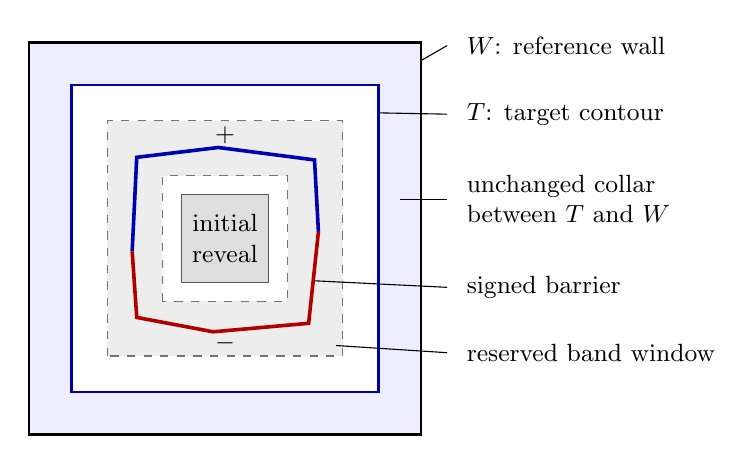
\begin{tikzpicture}[x=.83cm,y=.83cm,font=\small]
 \fill[blue!7] (-3,-3) rectangle (3,3);
 \fill[white] (-2.35,-2.35) rectangle (2.35,2.35);
 \fill[black!7] (-1.8,-1.8) rectangle (1.8,1.8);
 \fill[white] (-.96,-.96) rectangle (.96,.96);
 \draw[line width=.9pt] (-3,-3) rectangle (3,3);
 \draw[line width=.8pt,blue!65!black]
   (-2.35,-2.35) rectangle (2.35,2.35);
 \draw[dashed,black!55] (-1.8,-1.8) rectangle (1.8,1.8);
 \draw[dashed,black!55] (-.96,-.96) rectangle (.96,.96);
 \filldraw[fill=black!13,draw=black!65] (-.67,-.67) rectangle (.67,.67);
 \node[align=center] at (0,0) {initial\\reveal};
 \draw[line width=1.3pt,blue!70!black]
   (-1.42,-.2)--(-1.35,1.24)--(-.1,1.39)--(1.37,1.2)--(1.43,.1);
 \draw[line width=1.3pt,red!70!black]
   (1.43,.1)--(1.28,-1.3)--(-.18,-1.43)--(-1.35,-1.21)--(-1.42,-.2);
 \node at (0,1.58) {$+$};
 \node at (0,-1.6) {$-$};
 \node[anchor=west] at (3.55,2.95) {$W$: reference wall};
 \draw (3,2.72)--(3.4,2.95);
 \node[anchor=west] at (3.55,1.9) {$T$: target contour};
 \draw (2.35,1.92)--(3.4,1.9);
 \node[anchor=west,align=left] at (3.55,.6)
   {unchanged collar\\between $T$ and $W$};
 \draw (2.68,.6)--(3.4,.6);
 \node[anchor=west] at (3.55,-.75) {signed barrier};
 \draw (1.38,-.65)--(3.4,-.75);
 \node[anchor=west] at (3.55,-1.75) {reserved band window};
 \draw (1.7,-1.64)--(3.4,-1.75);
\end{tikzpicture}
\caption{One buffered source square, drawn schematically.  Dashed
squares delimit the reserved band window; the numerical stopping
levels are omitted.  The signed barrier separates the initial reveal
from $T$, with room for offsets and tip caps inside the window.
Changing the continuation beyond $W$ multiplies both laws on $T$ by
the same bounded-oscillation weight.}
\label{fig:buffer}
\end{figure}

\subsection{Deterministic barriers and soft fields}

For a bounded, piecewise regular profile $h$ with compact interior
support, set
\begin{equation}
 X_{\delta,h}=\delta^{15/8}\sum_{z}h(z)\sigma_z,
 \qquad
 U_{\delta,h}=
 \frac{\exp(X_{\delta,h})}{\E\exp(X_{\delta,h})}.
 \label{buf:weight}
\end{equation}
The expectation in the denominator is in the chosen homogeneous
reference law.  Profiles may be positive or negative.  Sampling their
fixed regular pieces on the lattice, with bounded lattice rounding of
their boundaries, is understood.

\begin{lemma}[Soft realization of a signed barrier]
\label{buf:barrier}
Fix a regular signed Jordan contour with finitely many sign arcs in an
interior square, a buffered outer target contour, and a more distant
square wall with a constant prescribed sign.  Given $\eta>0$, there is
a bounded piecewise regular
profile $h$, supported in arbitrarily small prescribed neighborhoods
of the signed contour, such that, for all sufficiently small $\delta$,
the law on the target with the contour pinned and the law tilted by
$U_{\delta,h}$ have total variation less than $\eta$.
The contour pins are not imposed in the latter law.  The profile and
all its nonzero tube widths are fixed before $\delta$ tends to zero.
The conclusion transfers through any unchanged outer buffer as in
\Cref{buf:tilt}, and can be applied successively to finitely many
disjoint buffered squares.
\end{lemma}

\begin{proof}
We compare the pinned law, the law with both pins and fields, and the
law with fields alone.  All error budgets in this proof may first be
divided by the finite transport constants in \Cref{buf:tilt}.

\paragraph{Fields in a pinned contour.}
Delete small neighborhoods of the finitely many sign switches.  Around
the remaining cores of the plus and minus arcs choose thin regular
tubes, with the matching field sign, and put zero field elsewhere.
The field has magnitude at least $h_0\delta^{15/8}$ on each tube core;
the finite number $h_0$ will be chosen last.  Fields on the inside of
the full pinned contour have no effect on its exterior.

Outside the contour, both the pinned law and the pinned-plus-field law
are between the following ordered laws.  For an upper law enlarge the
plus arcs into fully plus-pinned strips and omit the negative fields;
for a lower law use minus-pinned strips and omit the positive fields.
All original contour pins remain.  Strip shapes can be chosen as
regular bulges attached to just the corresponding sign arcs.  Their
ends stay away from the switches, and the outer wall is unchanged.
After integrating irrelevant components, the target components are
regular marked domains, possibly annular.  They converge back to the
original marked domain as the strip widths tend to zero.

Choose a square source contour $S_0$ beyond all strips and an
intermediate square cut $J$ between $S_0$ and the target, with fixed
pin-free collars.  At fixed positive strip widths,
\Cref{in:fields} gives convergence of the rescaled one-point functions
on $J$.  Their limits converge to those in the original domain when
the widths shrink.  They are uniformly bounded on $J$: its distance
from every pin is positive, and the fully wired one-arm bound controls
the absolute magnetization.  Consequently the difference of the
normalized magnetic sums on $J$ tends to zero.  In rescaled coordinates
this normalization is $\delta^{7/8}\sum_{z\in J}\sigma_z$, up to
fixed geometric factors.

For either of the two laws being compared, couple it in order below
the common upper law.  The magnetic difference is bounded by the full
upper-minus-lower difference.  The continuation from $S_0$ to the
target is identical in these comparisons, and has no field or changed
pin.  \Cref{in:ordered} therefore gives an arbitrarily small target-TV
distance.  This conclusion is uniform in $h_0$, because the extreme
pinned-strip laws do not depend on the field magnitude.

\paragraph{Pins in a soft field.}
Keep the positive tube widths just chosen.  Cover each arc core by
finitely many patches, each contained in the central third of a
square whose slightly larger buffered square is still inside the
matching-sign tube.  Consider first a plus patch and the comparison
law with free boundary on its larger square and homogeneous field
$h_0\delta^{15/8}$.

By the necklace input in \Cref{in:fields}, given $\xi>0$ there are
finite $K$ and $c>0$ such that, at sufficiently small mesh, with
probability at least $1-\xi$ the central square is surrounded by a
vertex circuit covered by at most $K$ critical FK clusters, each with
at least $c\delta^{-15/8}$ vertices.  Consecutive pieces may touch by
a nearest-neighbor step.  Equivalently, the event can be expressed
using connected subsets of that minimum size; it is then increasing
under addition of bonds.  The internal-bond law in the positive field
dominates the zero-field law.  Conditional on its internal clusters,
each qualifying cluster attaches to the plus ghost with probability
at least $\tanh(c h_0)$.  The usual conditional cluster formula, or
a union bound over the at most $K$ clusters, now gives a plus-spin
circuit with probability at least
\begin{equation}
 1-\xi-K\bigl(1-\tanh(c h_0)\bigr).
 \label{buf:necklace-plus}
\end{equation}
The same estimate holds for a larger matching positive field by
monotonicity.  Thus its failure probability can be made arbitrarily
small with a sufficiently large but finite $h_0$.

Across the buffer of the larger square, \Cref{in:ratio} compares this
local law to the actual one, uniformly in all common fields and
remote signs.  It multiplies the failure probability by a fixed
constant.  Matching pins inserted earlier inside the local chart
preserve the circuit event by monotonicity; other pins are covered by
the same comparison.  The argument for a minus patch is obtained by
spin flip.

Here is the coupling that turns the circuit estimate into a pinning
estimate.  Couple the law before a plus patch is pinned and the law
after it is pinned in stochastic order.  Start at the patch and
reveal, in order, the non-plus sites accessible from it by star
adjacency, together with their first plus boundary.  At each step
use the ordered conditional distributions of the next site.  This
is a finite adaptive spin reveal; conditional on its revealed spins,
the unobserved law is the original Gibbs continuation.  A
nearest-neighbor plus circuit in the lower configuration confines
the exploration before it reaches the target.  The separating plus
boundary is plus in both configurations.  The exterior conditional
laws are then identical and can be sampled together.  It follows
that the target-TV distance is at most the lower law's circuit
failure probability.  This uses a stopping reveal, rather than
conditioning on an arbitrarily selected random circuit.  For minus
pinning reverse the order.

Apply the construction to the finite patch cover, allocating the
variation budget among its members.  Pins still missing near sign
switches lie in finitely many small disks.  By \Cref{in:patch}, inserting
these pins changes the target law by an arbitrarily small amount,
uniformly in the fields and the other pins.  Thus the field-only law
and the pinned-plus-field law are close on the target.

The choices have the required order: first make the switch
neighborhoods small; next make the strips thin but of positive
width; next choose a sufficiently large finite $h_0$; finally choose
the mesh small enough.  The first comparison was uniform in $h_0$.
Combining the two comparisons proves the local statement.
\Cref{buf:tilt} transports each comparison to any allowed
continuation.  For finitely many disjoint squares, condition on all
other pins or fields and telescope; their differences remain beyond
the square's outer buffer.
\end{proof}

\subsection{Uniform replacement of bounded observables}

Fix concentric buffer geometries with inner scale $s$ and outer scale
$R$, where $R/s$ is a sufficiently large fixed number.  An inner
observable is supported in $B_s$, and an outer observable is supported
on or beyond $\partial B_{R/2}$.  There is room for a fixed-factor
buffer at either end.  In a half-plane chart the center is on the
limiting boundary line.  Constants denoted $c,C>0$ below depend only
on these fixed support and separation factors.  In particular, they
do not depend on an approximation tolerance.

\begin{lemma}[Finite soft-weight replacement]
\label{buf:soft}
In the preceding reference geometries, for every $\eta>0$ there is a
finite list of bounded piecewise regular profiles $h_1,\ldots,h_N$,
and a fine-mesh threshold, such that every inner observable $F_\delta$
with $\norm{F_\delta}_\infty\le1$ has coefficients
$c_1(\delta),\ldots,c_N(\delta)$ satisfying
\begin{equation}
 \sum_{i=1}^N|c_i(\delta)|\le1,
 \qquad
 \sup_{\norm{H_\delta}_\infty\le1}
 \left|\E[F_\delta H_\delta]
       -\sum_{i=1}^N c_i(\delta)
                    \E[U_{\delta,h_i}H_\delta]\right|<\eta.
 \label{buf:one-side}
\end{equation}
The supremum is over all outer observables, including the constant
one.  The profiles and threshold are independent of $F_\delta$ and
$H_\delta$.  The coefficients may depend on the mesh and on the
observable.  The analogous statement holds with the inner and outer
roles reversed.

Inner replacement profiles can be supported within distance $Cs$
of the center; outer replacement profiles can be supported where
$cR\le |z|\le CR$.  The two profile regions have a fixed relative
radial separation.  Each profile is supported in a compact interior
set avoiding the center, with additional positive clearances that
may depend on $\eta$.

More precisely, let $(F_{\alpha,\delta})_{\alpha=1}^p$ and
$(H_{\beta,\delta})_{\beta=1}^q$ be finite families of inner and outer
observables, all of sup norm at most one.  There are finite inner and
outer profile lists $(h_i)$ and $(g_j)$ and coefficient vectors
$c_{\alpha i}(\delta),d_{\beta j}(\delta)$ such that
\begin{gather}
 \sum_i|c_{\alpha i}(\delta)|\le1,\qquad
 \sum_j|d_{\beta j}(\delta)|\le1,\label{buf:matrix-mass}\\
 \left|\E[F_{\alpha,\delta}H_{\beta,\delta}]
 -\sum_{i,j}c_{\alpha i}(\delta)d_{\beta j}(\delta)
       \E[U_{\delta,h_i}U_{\delta,g_j}]\right|<\eta
 \quad\text{for every }\alpha,\beta.\label{buf:two-side}
\end{gather}
The same row and column vectors work throughout this matrix.  Adjoin
the zero profile, for which $U_{\delta,0}=1$, to each list.  A constant
observable can then be retained exactly; adjoining it to either family
controls all the separate means with the same coefficients.  The
profile lists and mesh threshold are independent
of the observables.  The preceding support bounds apply to both lists.
Parity and plane lattice-rotation symmetries may be imposed by averaging.
The same conclusions hold along the approaching-half-plane charts
described above.
\end{lemma}

\begin{proof}
We first prove the one-sided assertion.  Smooth the observable by
conditioning on a separating square contour at its end of the
buffer.  For the outer observable, a square just inside $B_{R/2}$
can be used.  The conditional mean is bounded by one, and replacing
the observable by that mean preserves its pairings with all tests on
the other side of the cut.

Break the contour at its corners and, in a boundary chart, at its
intersections with the physical boundary.  Choose intersections
transversely and away from corners, or include a coincident corner
in the same deletion.  Delete short pieces in small disks at these
points.  The values in a deleted piece can be assigned arbitrarily
in the far conditional law, at a cost tending to zero by
\Cref{in:patch}.  More explicitly, average the original bounded
contour function over the deleted spins conditional on the retained
ones.  For every assignment of the retained spins, compare the far
law for each deleted-spin assignment to a single prescribed one.
The uniform pointwise ratio bound controls the resulting pairing
error.  Comparing that prescribed law back to the conditional mixture
costs the same bound.  Thus the new pairing is again in the original
reference measure, with the conditionally averaged contour function.
This operation does not assert a pointwise approximation of
the observable.  It also handles the vanishing displacements of
intersection points in an approaching boundary chart.

The retained segments have positive distance from the physical edge
and from the far test.  Subdivide them into finitely many sufficiently
short straight pieces, and delete much smaller gaps at the subdivision
points by the same argument.  Each piece now lies strictly inside its
own square, and these squares have disjoint enlarged buffers.  The buffers may be thin: for adjacent pieces of length $\ell$ separated
by a gap $g$, one may take square half-sides just above $\ell/2$ and
outer walls at $\ell/2+g/4$, with strictly nested band and target levels
in between. The stopping theorem allows any such fixed positive
clearances \cite[Remark~7.1]{IsingToolkit}; its constants need not be uniform as $g/\ell$ shrinks.
Choose the piece lengths after the original corner and physical-edge
deletions, smaller than their positive geometric clearances. This also
keeps squares on different sides disjoint. All these sizes and their
number are fixed before the mesh limit.  The
observable, for the purpose of the desired pairings, has become a
bounded function of spins in these finitely many source squares.

In each square reveal an interior square containing its source piece
and apply the outward part of \Cref{in:transfer}.  Choose a separating
target square contour $T$ outside the stopping band, and a more
distant constant-sign reference wall $W$, both still inside the
square's buffer; see \Cref{fig:buffer}.  The theorem gives finitely
many deterministic regular signed barriers.  Off an exceptional
descriptor, adding the chosen barrier changes the reference target
law by the prescribed small total-variation amount, for every
realizable stopping transcript.

The actual continuation can include all other source squares, their
transcripts, and the physical boundary.  These data lie beyond $W$.
The law on $T$ is therefore tilted by the common weight in
\Cref{buf:tilt}, independently of the transcript and its replacement.
The per-transcript TV estimate transports to this continuation.
Its further law is the same given $T$.  The exceptional probability
is still small, by the buffered comparison for the band marginal.
Thus both required parts of the stopping theorem transport: the
exceptional-event estimate uses the band density, and the conditional
target estimate uses the common target-contour tilt.

Apply these comparisons successively to the finite family of source
squares.  Conditional on their transcripts the remaining law is
Gibbs with the revealed pins.  Each square's unchanged outer collar
permits the same conditional comparison, so the errors telescope.
After all barriers have been inserted, they separate the initially
observed spins from every far test.  The law for the latter is the
original reference law with just the selected deterministic signed
barriers imposed; it no longer depends on the transcript behind them.

Let $A_i$ be the good descriptor bins, with a joint index if several
squares are used.  The corresponding coefficient is
\[
 c_i(\delta)=\E[F_\delta\one_{A_i}],
 \qquad
 \sum_i|c_i(\delta)|
 \le\E[|F_\delta|\one_{\cup_i A_i}]\le1.
\]
Here $F_\delta$ denotes the bounded function after the initial
conditioning and deletions.  Its pairings already differ from the
original ones by only the allocated error.  Exceptional bins
contribute at most their probabilities.  We have therefore obtained
a signed combination of deterministic pinned laws with coefficient
mass at most one, uniformly against every bounded far test.

Apply \Cref{buf:barrier} to every member of the finite barrier list.
For a joint barrier choice, add the profiles in its disjoint squares.
The field-only measure is exactly the original reference measure
tilted by the single normalized weight for this sum profile.
Normalization is global; no product of local normalizing constants
is assumed.  The coefficient mass does not change.  Allocate the
remaining errors among the finitely many choices and squares.
This proves \eqref{buf:one-side}.

All source squares were placed on fixed-factor contours at the
observable's end of the original collar.  Consequently their
profiles remain within $Cs$ at the inner end, or between $cR$ and
$CR$ at the outer end, regardless of how small the deletion disks,
strip widths, or approximation tolerances are chosen.  They avoid
the center.  The deletion and subdivision choices put them strictly
in the interior, also in boundary charts.  This proves the support
claims.

If a finite symmetry group preserves the reference law and the
geometry, average the replacement over that group, with its
appropriate character for an odd observable.  Enlarge the finite
profile list by the corresponding images.  The sum of absolute
coefficients cannot increase.  In the plane this includes the
right-angle lattice rotations and spin flip; free boundary also
permits spin flip.

The two-sided finite-array assertion requires uniform integrability
when a soft weight replaces one of the original bounded tests.  We
give its proof after establishing the required moment bounds in
\Cref{buf:moments}.  The preceding one-sided construction is
independent of those bounds.
\end{proof}

\subsection{Moments and the order of the two replacements}

\begin{lemma}[Smeared moments and exponential tails]
\label{buf:moments}
Let $h_1,\ldots,h_m$ be fixed bounded piecewise regular profiles with
compact interior supports in a reference chart.  All joint polynomial
moments of the variables $X_{\delta,h_i}$ converge to the integrals
of the corresponding continuum spin correlations.  For every
$t<\infty$,
\begin{equation}
 \sup_{\delta\ \mathrm{small}}
 \E\exp\!\left(t\sum_{i=1}^m|X_{\delta,h_i}|\right)<\infty.
 \label{buf:exponential}
\end{equation}
Joint exponential expectations converge as well.  In particular the
weights in \eqref{buf:weight} have convergent normalizations and
uniformly integrable powers of every fixed positive order.

For two separated support regions with a fixed buffer, there is a
geometric constant $K$ such that
\begin{equation}
 \E[A U_{\delta,g}]\le K\E A
 \label{buf:weighted-tail}
\end{equation}
for every nonnegative function $A$ of the first region and every
normalized positive soft weight on the second.  The constant is
independent of $g$, its magnitude, and its complexity.
\end{lemma}

\begin{proof}
First consider one compact set.  Buffered comparisons reduce bounds
on nonnegative functions there to bounds in the plane, or to a fixed
homogeneous square reference.  The standard two-point estimate is
\[
 \delta^{-1/4}\bigl|\E[\sigma_z\sigma_{z'}]\bigr|
 \le C(|z-z'|\vee\delta)^{-1/4}
\]
in the plane.  Its singularity is integrable in two dimensions, so
the second moments of the smeared fields are uniformly bounded.
The buffered comparison gives the same conclusion in compact
interior parts of the other reference geometries, and hence bounded
first moments as well.

For a nonnegative profile $h$, the GHS inequality
\cite[Theorem~2]{GHS1970}, in the nonnegative-field form of
\cite[Theorem~3.6]{CGN2015}, gives in a homogeneous plus or free
reference, for $t\ge0$,
\[
 \log\E e^{tX_{\delta,h}}
 \le t\E X_{\delta,h}
       +\tfrac12t^2\Var(X_{\delta,h}).
\]
The coefficients on the right are uniformly bounded.  The negative
exponential is bounded by the corresponding positive one using
spin flip and monotonicity; minus boundary follows by spin flip.
Plane and half-plane references follow by taking the homogeneous
finite-volume limits.  Write a signed profile as $h=h_+-h_-$ and
apply Cauchy--Schwarz to the two exponentials.  Covering a compact
support by finitely many buffered squares and applying H\"older,
if necessary, proves \eqref{buf:exponential} for every finite profile
list.  These are also the smeared-field exponential estimates
included in \Cref{in:fields}; the argument explains why no sign
restriction on $h$ is needed.

We next justify moment convergence at diagonals.  In a homogeneous
plus or free reference, cluster coloring bounds the absolute spin
product mean by the probability that every insertion connects to
the boundary of a small square around it.  Choose that square's
radius to be a fixed fraction of the minimum of its distance to
another insertion and its distance to the physical boundary.
The squares can be taken disjoint.  Conditioning successively
outside them and using the fully wired one-arm upper bound gives
the product bound
\begin{equation}
 \delta^{-b/8}\left|\E\prod_{i=1}^b\sigma_{z_i}\right|
 \le C_b\prod_{i=1}^b(d_i\vee\delta)^{-1/8},
 \label{buf:product-arm}
\end{equation}
where $d_i$ is the indicated nearest-point or boundary distance.
Repeated lattice sites are allowed by taking the trivial arm at
radius $\delta$.  Fixed minus boundary is reduced to plus by spin
flip.

On compact interior sets, the right side of
\eqref{buf:product-arm} has uniformly integrable collision
singularities.  To see the relevant power counting, group close
points in dyadic clusters.  A cluster of $q\ge2$ points costs at most
singular degree $q/8$, while its relative coordinates have dimension
$2(q-1)$.  At every nontrivial cluster in the nested grouping,
$2(q-1)-q/8>0$.  Summing the resulting geometric series, from the
smallest clusters outwards, bounds the integral and makes the
contribution of tuples within distance $\varepsilon$ of a diagonal
tend to zero uniformly in $\delta$.  The same counting bounds the
lattice sums, with the final dyadic shell truncated at $\delta$.

Away from the diagonals, \Cref{in:fields} supplies separated-point
convergence, and the regular profile pieces give Riemann-sum
convergence.  Removing the small diagonal region now proves every
joint polynomial moment limit.  The exponential bound permits
uniform approximation by Taylor polynomials: for example the tail
after degree $N$ is bounded in expectation by
$2^{-N}\E e^{2|X_{\delta,h}|}$.  This proves convergence of exponential
expectations and their joint versions.  Jensen's inequality and
the bounded first moments keep each normalizing denominator bounded
away from zero.  Higher exponential moments therefore give the
asserted uniform integrability of normalized weights.

Finally, the buffered density-ratio bound implies
\[
 \E[A\mid\hbox{spins in the second region}]\le K\E A
\]
for every nonnegative $A$ in the first region: compare a fixed
second-region assignment to its unconditional mixture.  Multiply
by the nonnegative normalized second-region weight and integrate.
This proves \eqref{buf:weighted-tail}.  Arbitrarily large finite
fields are allowed in the pointwise estimate, and the bound does
not depend on the chosen profile.
\end{proof}

\begin{proof}[Completion of the proof of \Cref{buf:soft}]
For the finite families in \eqref{buf:two-side}, first choose the inner
replacements with a small error budget.  For each row $\alpha$, the
one-sided statement gives one vector $c_{\alpha i}$ that works for all
outer columns.  The inner profile list is finite and independent of
these rows.  By
\Cref{buf:moments}, choose a finite $Q\ge1$ such that the tails
\[
 \E\bigl[U_{\delta,h_i}
                \one_{\{U_{\delta,h_i}>Q\}}\bigr]
\]
are uniformly small for every profile in those lists and every
sufficiently small mesh.  Apply the outer one-sided replacement to
every $H_{\beta,\delta}$, choosing its error smaller by the factor $Q$.
It gives one vector $d_{\beta j}$ that works simultaneously against all
the bounded inner tests $(U_{\delta,h_i}\wedge Q)/Q$.  Thus the
coefficients factor by row and column, as required in
\eqref{buf:two-side}.  The unused fixed-factor buffer margin
allows its inner test region to contain the whole support of the
first replacement, rather than just the original $B_s$.

The truncation error against an original bounded outer observable
is bounded by the displayed tail.  Against any positive normalized
outer replacement it is bounded by a geometric constant times that
tail, by \eqref{buf:weighted-tail}.  The sum of absolute outer
coefficients is at most one.  Thus this error estimate was available
\emph{before} the outer profile list was chosen; no bound on the
eventual field strengths is needed.  Removing the truncations and
summing the allocated finite error budgets proves the two-sided
assertion, including pairings with the constant one.
\end{proof}

The support statements in \Cref{buf:soft} leave fixed relative
buffers between radial ends, even as the approximation error tends
to zero.  This feature, together with
\eqref{buf:weighted-tail}, will give uniform Hilbert-space norms in
the radial argument.  All fine-mesh thresholds here may depend on
the fixed scale ratio and the requested error.  No quantitative rate
of primary-field convergence, necklace convergence, or stopping-band
convergence has been used.

\section{Radial spectral estimates and uniform conditional averaging}
\label{sec:radial}

We now turn the finite soft-field replacement into an estimate for
conditional averaging of arbitrary bounded lattice observables.  All
measures in this section are at the nearest-neighbor critical point.
Recall that $P_RF$ is the conditional expectation of $F$ given the
cutting spins of $B_R(0)$.  The bulk estimate uses the response to a
fixed-plus disk to detect the leading nonconstant component.

\begin{proposition}[Uniform bulk conditional averaging]
\label{rad:operator}
There are constants $C<\infty$ and $\ell_0<\infty$ with the
following property.  Fix $\ell=R/s\geq\ell_0$.  For all sufficiently
large $s$, with its threshold allowed to depend on $\ell$, let $F$
be any bounded lattice function supported in $B_s(0)$.  Put
\[
  m(F)=\E_{\mathbb C}F,
  \qquad
  d_R(F)=\E^+_{\mathrm{disk}(4R)}F-m(F).
\]
Then
\begin{align}
 |d_R(F)|&\leq C(s/R)^d\|F\|_\infty,\label{eq:rad-response}\\
 \|P_RF-m(F)\|_\infty
   &\leq C|d_R(F)|+C(s/R)^p\|F\|_\infty,
 \label{eq:rad-operator}
\end{align}
with
\[
 (d,p)=
 \begin{cases}
 (1,3),&F\text{ even and invariant under right-angle rotations},\\
 (1,2),&F\text{ even},\\
 (1/8,9/8),&F\text{ odd}.
 \end{cases}
\]
The constants are independent of every sufficiently large fixed
ratio.  The same conclusion holds along ratios tending to a fixed
$\ell\geq\ell_0$, after harmless changes in the thresholds.
\end{proposition}

The exponent $p=3$ in the square-symmetric even sector is essential for
bulk interactions: summing translated local terms in a larger block
costs two powers of the scale ratio.  A remainder with exponent two
would not give the contraction needed in Section~\ref{sec:renormalization}.
For a marked observable there is no such area factor; the other two
estimates have the required strict inequality $p>d$.

We prove the proposition by representing separated pairings in a radial
Hilbert space.  The spin formulas determine its low spectrum, and a
charge cancellation supplies the square-symmetric gain from exponent
two to three.  Uniform Hilbert norms for the soft weights then make
these spectral bounds apply to the finite dictionaries, independently
of their complexity.  Finally a fixed calibration observable detects
the disk component.  The half-plane version, proved at the end of the
section, gives the corresponding boundary estimate.

\subsection{The radial Hilbert space}

Write $\mathcal G$ for either the plane or the upper half-plane, with
homogeneous fixed or free boundary conditions in the latter case.  A
point state is a finite product
\[
   S_X=\prod_{x\in X}\sigma(x),
   \qquad X\subset\mathcal G\cap\{0<|z|<1\},
\]
at distinct points.  The empty state is denoted by $\one$.  We use the
continuum spin normalization in the reference limits; an overall
per-spin constant will not affect any assertion below.  Set
$\iota(z)=1/\overline z$.  On the linear span of point states define
\begin{equation}
 \langle S_Y,S_X\rangle_{\rm rad}
 =\left(\prod_{y\in Y}|y|^{-1/4}\right)
   \E_{\mathcal G}\left[
       \prod_{y\in Y}\sigma(\iota(y))\prod_{x\in X}\sigma(x)
   \right],
 \label{eq:rad-form}
\end{equation}
with the usual conjugation on the coefficients of the first argument.
The primary factors in this definition are those for a field of
dimension $1/8$.

The form is positive semidefinite.  Indeed, Euclidean reflection
positivity for the nearest-neighbor reference model
\cite{FILS1978} passes from reflection-symmetric critical lattice domains to
the separated-point continuum correlations.  In the half-plane the
reflecting line can be chosen perpendicular to the physical boundary,
with both lines lattice aligned before taking the limit.  A conformal
map conjugates that line reflection to reflection in the unit
semicircle and preserves the half-plane.  The analogous statement in
the plane uses the spherical covariance of the spin formula and a
M\"obius map taking a line to the circle.  Transformation of the field
factors gives exactly \eqref{eq:rad-form}.  This establishes positivity
also for complex linear combinations.  Quotienting by the null space
and completing will give a Hilbert space $\mathcal H$.

For $0<t\leq1$, initially on point states, put
\begin{equation}
       D_t S_X=t^{|X|/8}S_{tX}.
 \label{eq:rad-dilation}
\end{equation}
Covariance under scaling shows that $D_t$ is symmetric for
\eqref{eq:rad-form}, and $D_tD_u=D_{tu}$.  We check the contraction
property before passing to the quotient.  For a finite linear
combination $v$, Cauchy--Schwarz for the positive semidefinite form gives
\[
 \|D_t v\|_{\rm rad}^{2}
   =\langle v,D_{t^2}v\rangle_{\rm rad}
   \leq\|v\|_{\rm rad}\|D_{t^2}v\|_{\rm rad}.
\]
For each such $v$, the quantities $\|D_u v\|_{\rm rad}$ remain bounded
as $u\downarrow0$.  This follows directly from the spin formulas: in
the plane each squared product matrix element is a finite sum starting
at a nonnegative power of $u$, as computed in
\eqref{eq:rad-plane-expansion} below; in the half-plane the height
factors cancel the dilation factors and the cross factors have a
finite limit, as in \eqref{eq:rad-halfplane-formula}.  There is therefore
no spectral assumption in this boundedness observation.  Iterating the
last inequality yields
\[
 \|D_t v\|_{\rm rad}
 \leq \|v\|_{\rm rad}^{1-2^{-n}}
       \|D_{t^{2^n}}v\|_{\rm rad}^{2^{-n}}
 \longrightarrow \|v\|_{\rm rad}.
\]
If $v$ is null, the first inequality already says that $D_t v$ is null.
Consequently $D_t$ descends to a self-adjoint contraction on
$\mathcal H$.  It is positive, since
$D_t=D_{\sqrt t}^{2}$.  Continuity of separated-point correlations
gives strong continuity at $t=1$ on point states, and then on
$\mathcal H$ by contraction. Apply the self-adjoint semigroup theorem to
$s\mapsto D_{e^{-s}}$, using the underlying real Hilbert space and the
complex-linearity of this family; see
\cite[Theorem~7.3.10 and (7.3.9)]{BuehlerSalamon2016}.
Contraction makes its generator nonpositive. The spectral calculus
\cite[Theorem~6.4.1 and Section~6.5]{BuehlerSalamon2016} therefore gives
a nonnegative self-adjoint operator $\Delta$ such that
\begin{equation}
                     D_t=t^\Delta.
 \label{eq:rad-generator}
\end{equation}
The vacuum $\one$ has norm one.  Spin flip in the plane and in the free
half-plane, and rotations in the plane, act isometrically and commute
with every $D_t$.

\subsection{A charge identity}

We give the algebraic cancellation needed to exclude a
rotation-invariant contribution of dimension two.  For a list
$X=(z_1,\ldots,z_n)$ of distinct complex numbers, define
\[
 w_X(\mu)=\prod_{i<j}|z_i-z_j|^{\mu_i\mu_j/2},
 \qquad
 W_s(X)=\sum_{\substack{\mu_i\in\{-1,1\}\\\sum_i\mu_i=s}}
                    w_X(\mu).
\]
An impossible charge has weight zero; on the empty list $W_0=1$.
For an even nonempty list let $\E_0$ mean expectation with probability
weights $w_X(\mu)/W_0(X)$ on charge-zero assignments.

\begin{lemma}[Charge cancellation]
\label{rad:identity}
For every even list $X$,
\begin{equation}
 \E_0\left|\sum_i\mu_i z_i\right|^2
       =4\left(\frac{W_2(X)}{W_0(X)}\right)^2.
 \label{eq:rad-charge-identity}
\end{equation}
For the empty list both sides are zero.
\end{lemma}

\begin{proof}
We first prove a polynomial identity.  On a set $I$ of $2m$ points,
write $D_+(\mu)$ and $D_-(\mu)$ for the Vandermonde determinants on
the points with the indicated signs, and put
\[
 V_s(I)=\sum_{\sum_{i\in I}\mu_i=s}|D_+(\mu)D_-(\mu)|^2.
\]
Then
\begin{equation}
 \sum_{\sum\mu_i=0}|D_+(\mu)D_-(\mu)|^2
                  \left|\sum_i\mu_i z_i\right|^2
                         =2V_2(I).
 \label{eq:rad-vandermonde}
\end{equation}
Here and below the Vandermonde on an empty set is one.

For completeness, work in the exterior algebra of
$\mathbb C^{2m}\otimes\mathbb C^2$, with orthonormal site and color
basis $e_i\otimes e_\pm$.  Define
\[
 p_k^\pm=\sum_{i\in I}z_i^k e_i\otimes e_\pm,
 \qquad
 \Psi=\bigwedge_{k=0}^{m-1}(p_k^+\wedge p_k^-).
\]
Let $Q$ project to the subspace with exactly one exterior factor at
each site.  Both $\Psi$ and $v=Q\Psi$ are invariant under simultaneous
$SU(2)$ transformations of the colors: each two-column wedge is
multiplied by the determinant, which is one, and $Q$ commutes with
color transformations.  In the basis indexed by one sign per site,
$v$ has only balanced coordinates, whose absolute values are
$|D_+(\mu)D_-(\mu)|$.

Let $\tau_1,\tau_2,\tau_3$ be the Pauli matrices and let
$A_j=\sum_i z_i\tau_j^{(i)}$ act on this subspace.  The Gram matrix
$\langle A_jv,A_kv\rangle$ is invariant under every real
three-dimensional rotation, because $v$ is $SU(2)$ invariant.
It is therefore a scalar multiple of the identity.  For
$A_+=(A_1+iA_2)/2$ we obtain
\begin{equation}
                  \|A_3v\|^2=2\|A_+v\|^2.
 \label{eq:rad-su2}
\end{equation}
The left side is the left side of \eqref{eq:rad-vandermonde}.
On the full exterior algebra $A_+$ is the derivation sending
$e_i\otimes e_-$ to $z_i e_i\otimes e_+$ and sending a plus factor
to zero; this derivation commutes with $Q$.  Applied to $\Psi$, all
terms vanish by repeated columns except the replacement
$p_{m-1}^-\mapsto p_m^+$.  The remaining plus columns have degrees
$0,\ldots,m$, and the remaining minus columns degrees
$0,\ldots,m-2$.  Thus the absolute values of its projected coordinates
are exactly the Vandermonde products in $V_2(I)$.  Equation
\eqref{eq:rad-su2} proves \eqref{eq:rad-vandermonde}.  When $m=0$ the
identity is the trivial equality $0=0$.

We now multiply the numerator on the left of
\eqref{eq:rad-charge-identity} by $W_0(X)$.  In the resulting sum over
two balanced assignments $\mu,\nu$, partition the sites into the
agreement set $A=\{i:\mu_i=\nu_i\}$ and its complement $B$.
Both restrictions of $\mu$ are balanced, since
\[
 \sum\mu_i=\sum\nu_i=0
 \quad\Longrightarrow\quad
 \sum_{i\in A}\mu_i=\sum_{i\in B}\mu_i=0.
\]
The factors joining $A$ to $B$ cancel in $w_X(\mu)w_X(\nu)$.
For either group $I=A,B$, put
$q(I)=\prod_{i<j\in I}|z_i-z_j|^{-1}$.  The remaining factor in that
group is
\[
 \prod_{i<j\in I}|z_i-z_j|^{\mu_i\mu_j}
                      =q(I)|D_+(\mu)D_-(\mu)|^2.
\]
If $M_I=\sum_{i\in I}\mu_i z_i$, the mixed terms in
$|M_A+M_B|^2$ sum to zero by reversal of all signs on one balanced
group.  Equation~\eqref{eq:rad-vandermonde} therefore shows that the
sum under consideration equals
\begin{equation}
 2\sum_{\substack{A\sqcup B=X\\|A|,|B|\text{ even}}}q(A)q(B)
       \bigl[V_2(A)V_0(B)+V_0(A)V_2(B)\bigr].
 \label{eq:rad-agreement}
\end{equation}
The same grouping applied to two charge-two assignments has charge
two on $A$ and charge zero on $B$.  Hence the first sum in brackets
is $W_2(X)^2$.  Applied to charges two and minus two, it has charge
zero on $A$ and charge two on $B$, so the second sum is
$W_2(X)W_{-2}(X)$.  Sign reversal gives $W_{-2}=W_2$.
Thus \eqref{eq:rad-agreement} is $4W_2(X)^2$; division by
$W_0(X)^2$ proves the assertion.
\end{proof}

\subsection{The low radial spectrum}

\begin{proposition}[Low spectrum]
\label{rad:spectrum}
Let $\Pi_0$ be projection onto the vacuum.  The following statements
hold on the indicated closed sectors of $\mathcal H$.
\begin{enumerate}[label=\textnormal{(\roman*)}]
\item In the even plane sector there is a nonzero rank-one projection
      $\Pi_1$ at dimension one and
      \[
      \|D_t-\Pi_0-t\Pi_1\|\leq t^2.
      \]
      On the subspace invariant under rotation by $\pi/2$, the right
      side may be replaced by $t^3$.
\item In the odd plane sector there is a nonzero rank-one projection
      $\Pi_{1/8}$ and
      \[
      \|D_t-t^{1/8}\Pi_{1/8}\|\leq t^{9/8}.
      \]
\item In the fixed half-plane, and in the even sector of the free
      half-plane,
      \[
                       \|D_t-\Pi_0\|\leq t^2.
      \]
\end{enumerate}
The vacuum matrix element is
$\langle v,\Pi_0w\rangle
=\overline{\E v}\,\E w$.
\end{proposition}

\begin{proof}
We first record how pointwise expansions determine the spectral
assertions.  For $v$ in the dense span of point states,
\[
       \langle v,D_tv\rangle
             =\int_{[0,\infty)}t^q\,d\nu_v(q),
       \qquad \nu_v\geq0.
\]
Suppose its expansion consists of finitely many specified powers
below $p$, with an $O_v(t^p)$ remainder.  The limit at zero identifies
the mass at zero.  After removing that mass, positivity excludes
spectral mass on each interval below the first remaining specified
power: any positive mass on a compact subinterval there would decay
more slowly than the expansion allows.  Dividing by that first power
and taking a limit identifies its atom.  Repeating this argument
identifies the subsequent atoms and excludes the intervening
intervals, including the interval up to $p$.  Polarization identifies
their matrix elements.  If the excluded spectral projection vanishes
on the dense point-state span, it vanishes on the entire Hilbert
space.  Consequently no uniformity of the constants in the
point-state remainders is needed for this step.

Normalize the plane spin field temporarily so that its two-point
function is $|z-w|^{-1/4}$.  The exact formula for an even list $Z$ is
\[
         \bigl(\E S_Z\bigr)^2=2^{-|Z|/2}W_0(Z).
\]
For lists $X=(x_i)_{i=1}^k$ and $Y=(y_j)_{j=1}^l$ of the same
parity, the reflected, dilated matrix element
$F_{X,Y}(t)=\langle S_Y,D_tS_X\rangle$ consequently satisfies
\begin{align}
 F_{X,Y}(t)^2
 &=2^{-(k+l)/2}\sum_s t^{s^2/4}
   \sum_{\substack{\sum_i\mu_i=s\\\sum_j\nu_j=-s}}
       w_X(\mu)w_Y(\nu)
       \prod_{i,j}|1-tx_i\overline y_j|^{\mu_i\nu_j/2}.
 \label{eq:rad-plane-expansion}
\end{align}
Indeed the inner dilation contributes $t^{(s^2-k)/4}$ to the spin
correlation square and $t^{k/4}$ from \eqref{eq:rad-dilation}.
Inversion of the outer list contributes powers of $|y_j|$ that
cancel its primary factors and the cross-distance powers.  This
leaves exactly \eqref{eq:rad-plane-expansion}.  Each remaining cross
factor has a convergent integer-power expansion near zero.

For odd lists the lowest charges are $s=\pm1$.  Their leading
coefficients are equal and factor as $W_1(X)W_1(Y)$.  Taking the
positive square root gives
\[
 F_{X,Y}(t)=a(X)a(Y)t^{1/8}+O_{X,Y}(t^{9/8}),
\]
where $a$ is nonzero, since $W_1$ is positive.  In the even sector
the charge-zero term has leading coefficient
$m(X)^2m(Y)^2$, where $m(X)=\E S_X>0$ for a nonempty even list.
The coefficient linear in $t$ from charge zero vanishes by sign
reversal on one list.  The charges $s=\pm2$ therefore give
\begin{equation}
 F_{X,Y}(t)
  =m(X)m(Y)+m(X)\frac{W_2(X)}{W_0(X)}
                  m(Y)\frac{W_2(Y)}{W_0(Y)}\,t
      +O_{X,Y}(t^2).
 \label{eq:rad-even-expansion}
\end{equation}
The order-one matrix has rank one and is nonzero already for a
two-spin state.  Empty states are handled directly: their pairings
are the means, and they have no nonconstant coefficient.

For the improved even estimate, set
$A_X=\sum_i\mu_i x_i$ and $A_Y=\sum_j\nu_j y_j$ under their
independent charge-zero weights.  The linear cross exponent is
\[
               -\tfrac12 t\operatorname{Re}(A_X\overline{A_Y}).
\]
The quadratic term in the logarithm has angular frequency two.
Averaging rotation of $X$ over the four right-angle rotations
therefore leaves, from the square of the linear term, only
\[
 \frac1{16}\E_0|A_X|^2\E_0|A_Y|^2t^2.
\]
The order-$t$ correction to the $s=\pm2$ cross factors has angular
frequency one, and so supplies no invariant coefficient of order
$t^2$.  Put $a_X=W_2(X)/W_0(X)$ and similarly for $Y$.
Lemma~\ref{rad:identity} says that the invariant expansion of the
correlation square, relative to its constant term, is
\[
                  1+2a_Xa_Yt+(a_Xa_Y)^2t^2+O(t^3).
\]
The order-$t$ coefficient before averaging is already rotation
invariant.  We may therefore expand the square root first and then
average: its invariant quadratic coefficient is
\[
             \tfrac12(a_Xa_Y)^2
                    -\tfrac18(2a_Xa_Y)^2=0.
\]
Thus the remainder in \eqref{eq:rad-even-expansion} is $O(t^3)$
after projecting one state to right-angle invariance.  This proves
all the plane spectral statements by the preceding positivity
argument.  It also identifies $\Pi_0$ as the vacuum projection.

In the half-plane, the squares of the fixed/free spin formulas
have the form
\begin{equation}
 c_n\prod_i(2\operatorname{Im}z_i)^{-1/4}
       \sum_{\mu_i=\pm1}\chi_n(\mu)
       \prod_{i<j}
       \left|\frac{z_i-z_j}{z_i-\overline z_j}\right|^{\mu_i\mu_j/2}.
 \label{eq:rad-halfplane-formula}
\end{equation}
For fixed plus boundary, $c_n=2^{-n/2}$ and $\chi_n=1$.  For free
boundary and even $n$, $c_n=(-1)^{n/2}2^{-n/2}$ and
$\chi_n=\prod_i\mu_i$.  These are the fixed/free formulas in
Proposition~\ref{in:fields}.  Fixed minus follows by spin flip.

In a reflected pairing the inner height factors cancel the
dilation factor, and the outer height factors cancel the primary
factors exactly.  At $t=0$ the cross factors are one.  Since
$c_{k+l}=c_kc_l$ for all list lengths in the fixed case and for even
list lengths in the free case, the constant term is exactly the
product of the separate correlation squares.

The linear cross term is odd under simultaneous reversal of the
signs on either list.  Internal weights are invariant under that
reversal; so is $\prod_i\mu_i$ when the list is even.  The linear
term therefore vanishes.  The separate means are nonzero for every
fixed-boundary point product, and for every even free-boundary point product.
This follows from the positive one- and two-point functions and
the ferromagnetic product inequalities, or directly from the
formulas.  Taking the square root, with the sign prescribed by
fixed minus where necessary, gives
\[
       F_{X,Y}(t)=m(X)m(Y)+O_{X,Y}(t^2).
\]
The spectral extraction argument again applies, proving the
boundary statement.  The zero state and linear combinations are
included by direct pairing and polarization.
\end{proof}

\subsection{Soft fields as uniformly bounded states}

\begin{lemma}[Uniform radial norms]
\label{rad:soft-norm}
Consider the continuum normalized soft weights supplied by
Lemma~\ref{buf:soft}.  If their supports lie on the inner side of a
radial circle with a fixed relative buffer, each weight defines an
element of $\mathcal H$ of norm at most a constant depending only
on that buffer geometry.  The bound is independent of the bounded
profile, its magnitude, and the accuracy used to choose the finite
dictionary.  A linear combination with total absolute coefficient
sum at most $B$ has norm at most $CB$.
\end{lemma}

\begin{proof}
For a fixed profile, Lemma~\ref{buf:moments} constructs the
exponential by its polynomial series.  Integrated spin products
belong to the completion of the point-state span: remove small
diagonals, approximate the remaining integrals by finite sums of
point states, and then restore the diagonals.  The integrable
product-arm bounds used in Lemma~\ref{buf:moments} control this
procedure in the squared Hilbert norm as well, since inner and
reflected outer supports are separated.  Exponential-series tails
converge in that norm by the same moment bounds; absolute values
are dominated by a nonnegative majorant profile and the
nonnegative fixed-plus or free spin correlations.  Fixed minus is
reduced to plus by reversing the profile.  This proves membership
in $\mathcal H$, not merely existence of the ordinary expectation.

Let $U$ be such a normalized positive weight and let $\mathcal JU$
be its reflected weight, including the Jacobian and primary
factors in the reflected profile.  Conformal covariance gives
$\E\mathcal JU=\E U=1$.  On the lattice, the separated-support
ratio estimate bounds the conditional mean of either normalized
positive weight, given the spins supporting the other, by a fixed
constant.  Applying this estimate to fixed-profile approximations
and taking the limit by Lemma~\ref{buf:moments} gives
\[
                  \|U\|_{\rm rad}^2=\E[U\mathcal JU]\leq C.
\]
Crucially, the lattice bound does not depend on the weights'
amplitudes.  It therefore holds uniformly over all the finite
dictionaries, including dictionaries obtained with smaller
approximation errors.  The triangle inequality proves the last
assertion.
\end{proof}

\subsection{Calibration and the lattice operator estimates}

We first record the microscopic one-point consequence of the
reference-field convergence that will also be used in the
renormalization argument.  The lattice disk below is centered at
the observation site and is invariant under the square symmetries.

\begin{lemma}[Nonzero disk responses]
\label{rad:calibration}
Let $\mathcal O_{1/8}(z)=\sigma_z$ and let
$\mathcal O_1(z)=e(z)$ be the symmetric average of the four incident
bond products.  With $m$ denoting infinite-plane critical
expectation, there are nonzero real constants $\kappa_d$ such that
\begin{equation}
 \lim_{R\to\infty}R^d\left(
       \E^+_{\mathrm{disk}(4R)}\mathcal O_d(0)
                             -m(\mathcal O_d(0))\right)=\kappa_d,
 \qquad d\in\{1/8,1\}.
 \label{eq:rad-micro-calibration}
\end{equation}
\end{lemma}

\begin{proof}
Rescale the disk to radius four and apply the spin and scalar-energy
one-point convergence in the reference input
Proposition~\ref{in:fields}.  Plane centering is the standard energy
centering in this one-point statement.  The fixed-boundary
magnetization at the center is positive, and the plane-centered
scalar-energy one-point function there is nonzero.  Averaging the
four incident orientations preserves its common scalar limit.
These observations give \eqref{eq:rad-micro-calibration}; no rate
of convergence is used.
\end{proof}

\begin{proof}[Proof of Proposition~\ref{rad:operator}]
Normalize $\|F\|_\infty\leq1$.  For any assignment $\tau$ on the
cutting contour at radius $R$, condition first on a separating
contour at a fixed smaller radius, for example $R/2$.  Relative
to the critical plane law, its distribution induced by $\tau$
has a density $H_\tau$ with
\[
                  \E H_\tau=1,\qquad 0\leq H_\tau\leq C.
\]
The bound follows from the ratio estimate across the intervening
fixed-modulus buffer and is uniform over every configuration
$\tau$, not just typical configurations.  The same construction
represents disk-plus expectation by a normalized density $H_D$
on that contour, with the same kind of bound.  The Markov property
therefore identifies
\begin{equation}
 \begin{split}
 P_RF(\tau)-m(F)&=\Cov(F,H_\tau),\\
 d_R(F)&=\Cov(F,H_D).
 \end{split}
 \label{eq:rad-test-columns}
\end{equation}

Apply the finite-matrix assertion \eqref{buf:two-side} to these
pairings, scaling the columns by their common sup-norm bound and
adjoining a constant row and column to control the separate means.
It gives one coefficient vector per row and per column, each with
bounded total absolute mass.  Lemma~\ref{buf:moments} passes each
fixed dictionary to the continuum.  The resulting inner and outer
states have uniformly bounded norms by Lemma~\ref{rad:soft-norm}.
Their supports lie at radial
ends of radii $C_1s$ and $c_1R$, where $C_1,c_1>0$ do not depend
on replacement accuracy.  After rescaling the radial ends, the
dilation parameter is
\[
                         t=\frac{C_1s}{c_1R}.
\]
We choose $\ell_0$ large enough that $t<1$.  Parity and, when
needed, right-angle invariance are imposed by averaging the
inner replacements.  These projections commute with $D_t$, so
no symmetry of the outer density is required.  Subtracting the
separate means removes the vacuum term.

For sufficiently fine mesh, every such finite matrix is therefore,
to arbitrarily small absolute error, a matrix of the form
\begin{equation}
                 t^d a_i b_j+E_{ij},
                 \qquad |a_i|,|b_j|\leq C,
                 \qquad |E_{ij}|\leq Ct^p,
 \label{eq:rad-rank-one-matrix}
\end{equation}
by Proposition~\ref{rad:spectrum}.  Coefficients in the finite
dictionaries may depend on the mesh; along an arbitrary sequence
we pass to a subsequence on which they converge.  Neither this
argument nor \eqref{eq:rad-rank-one-matrix} asserts convergence in
Hilbert norm of the original lattice observables.  In particular,
the first inequality in the proposition follows at once from
the disk column.

To obtain the second inequality we show that the disk column has
$|b_D|$ bounded away from zero.  Adjoin a fixed inner calibration
row: in the odd sector take a spin smeared against a nonnegative
profile in a small interior box; in the even sector take a product
of spins smeared in two small disjoint boxes, and average rotations
when appropriate.  Normalize these at the inner length scale.
They are fixed states of bounded Hilbert norm.  Lemma~\ref{buf:moments}
and truncation allow them to be paired with the same outer
replacements as the bounded row $F$.  Uniform control of the
truncation tails against normalized positive outer weights follows
from their separated-support density-ratio bound.

Their connected disk responses have a nonzero leading coefficient
of order $t^d$.  For the odd calibration this is the positive bulk
magnetization in a large fixed-plus disk.  For the even calibration,
the two-point case of \eqref{in:halfplane-plus}, with
$q=|z-w|/|z-\overline w|$, gives the explicit ratio
\[
 \frac{G_{2,\mathbb H}^{+}(z,w)}{G_{2,\mathbb C}(z,w)}
   =(1+q)^{1/2}(1-q^2)^{-1/8}
   =1+\frac q2+O(q^2).
\]
Here $G_{2,\mathbb C}(z,w)=|z-w|^{-1/4}$ in the normalization of
Proposition~\ref{in:fields}; the ratio is independent of the overall
spin normalization.  In a disk of radius $H$ centered at zero, the
same formula holds with
\[
 q=q_H(z,w)=\frac{H|z-w|}{|H^2-z\overline w|}
           =\frac{|z-w|}{H}+O(H^{-3})
\]
for points in the two fixed boxes.  Indeed a M\"obius map to the
half-plane gives this $q_H$, and covariance cancels the primary
factors between the disk and plane two-point functions.  The
coefficient of $H^{-1}$ in their difference is therefore
$\tfrac12|z-w|^{3/4}>0$ in the displayed normalization.  Smearing
with the fixed positive profiles gives the connected calibration response
\begin{equation}
                  c_*t^d+o(t^d),\qquad c_*>0,
 \label{eq:rad-disk-detection}
\end{equation}
as $t\downarrow0$.  This qualitative asymptotic is sufficient for
detection; it does not require a lattice convergence rate.
Rotation averaging preserves the positive leading coefficient.

Include this calibration row, the row $F$, the disk column, and
the column $H_\tau$ in one finite matrix.  For all sufficiently
small $t$, \eqref{eq:rad-disk-detection} and
\eqref{eq:rad-rank-one-matrix}, with replacement error smaller
than $t^p$, give
$|a_{\rm cal}b_D|\geq c>0$.  Since
$|a_{\rm cal}|\leq C$, this implies $|b_D|\geq c/C$.
Every other column has $|b_j|\leq C$, whence
\[
        |t^d a_Fb_\tau+E_{F,\tau}|
             \leq C|t^d a_Fb_D+E_{F,D}|+Ct^p.
\]
By \eqref{eq:rad-test-columns} this is
\eqref{eq:rad-operator}, first in the fine-mesh limsup sense.

Finally suppose a claimed lattice bound, with a slightly larger
constant, failed at arbitrarily large $s$ for the fixed ratio.
Choose the failing functions and, for the supremum estimate,
failing contour configurations along that sequence.  Apply the
finite-matrix argument just given to those rows and columns;
the finite dictionaries are uniform over the chosen functions.
Choose their accuracy below the fixed remainder scale $t^p$ and
then take the fine-mesh limit.  This contradicts the limsup bound.
It supplies a threshold uniform over $F$ and $\tau$.  The same
argument applies when the ratios approach the fixed ratio,
since all geometric buffers retain their positive clearances.
The constants used in the spectral and calibration estimates are
uniform for all sufficiently small $t$, hence for all sufficiently
large fixed ratios, as asserted.
\end{proof}

\begin{samepage}
\begin{proposition}[Uniform boundary conditional averaging]
\label{rad:boundary}
Fix support and separation factors, including a constant $C_0$.
There are $C<\infty$ and $\ell_0<\infty$ such that the following
holds.  For each fixed $\ell=R/s\geq\ell_0$, there are a lower
threshold for $s$, a sufficiently large chart-window factor, and
a sufficiently small flatness threshold, all allowed to depend
on $\ell$ but not on the boundary orientation.  Suppose a physical
boundary point lies within $C_0s$ of the common center of the
support and cutting squares, and that throughout the chart
window the boundary is a single $C^1$ graph with slope deviation
from its tangent below that threshold.  Retain its homogeneous
nearest-neighbor boundary type in the conditional averaging.
Then, for every bounded $F$ supported in the inner square,
\begin{equation}
               \inf_{c\in\mathbb R}\|P_RF-c\|_\infty
                       \leq C(s/R)^2\|F\|_\infty
 \label{eq:rad-boundary-operator}
\end{equation}
in fixed boundary conditions.  The same holds for even $F$ in
free boundary conditions.  For complex $F$, take $c\in\mathbb C$
and adjust the constant harmlessly.
\end{proposition}
\end{samepage}

\begin{proof}
First take a straight boundary and a fixed homogeneous reference
half-plane law.  As in \eqref{eq:rad-test-columns}, represent each
cutting-contour assignment on a slightly inner contour by a
bounded normalized density relative to that law.  The physical
boundary type is identical in both laws; only the artificial cut
is changed.  Lemma~\ref{buf:soft} replaces the resulting pairings
by uniformly bounded radial states.  Subtract the reference mean
of $F$, so that the vacuum projection disappears.  The boundary
case of Proposition~\ref{rad:spectrum} bounds every remaining
pairing by $C(s/R)^2\|F\|_\infty$.  This is uniform over the
arbitrary cut assignment.  For fixed minus use spin flip; in the
free case use the even projection on the inner state.

The radial origin may be moved to the nearby physical boundary
point.  The support then lies within a square of radius
$(1+C_0)s$ about that point, while the outer test remains at a
distance comparable to $R$ if $\ell_0$ is large enough.
This changes only the fixed geometric constants.  The limiting
half-plane may be rotated after taking the continuum limit;
covariance makes its radial estimate independent of orientation.
The lattice buffers themselves may remain axis-parallel.

For locally graphical curved boundaries use the reference-chart
construction in Section~\ref{sec:buffers}.  Its capped reference
domain agrees with the actual physical edge on the buffer under
consideration, so the bounded-density representation remains
valid.  If the asserted thresholds did not exist for a fixed
ratio, one could choose a sequence of failing examples with
$s\to\infty$, graph slope deviations tending to zero, and chart
windows increasing without bound.  After rescaling and passing
to a subsequence, the tangent orientations converge and the
charts converge locally to a half-plane.  The contour
replacement and moment convergence statements hold in these
charts, with the fixed positive radial buffers described in
Lemma~\ref{buf:soft}.  The same finite-matrix limsup argument as
in Proposition~\ref{rad:operator} would then contradict the
straight-boundary bound.  This proves the existence of a finite
window, a positive flatness threshold, and a finite mesh
threshold.  Compactness of the set of orientations makes these
thresholds uniform in orientation.  No rate for convergence of
the graph or of a nearest-neighbor correlation is needed.
\end{proof}

\begin{remark}
The order of choices in the two propositions is important.  The
large ratio is fixed first; approximation tolerances smaller than
its spectral remainder are then fixed, and only afterward is the
lattice scale required to be sufficiently large.  The geometric
and spectral constants are uniform over large fixed ratios, but
no uniform rate in that last fine-mesh passage has been asserted.
For a fixed compact $C^2$ Jordan boundary, the graph and flatness
conditions of Proposition~\ref{rad:boundary} hold on all
sufficiently small physical windows, uniformly along the
boundary.
\end{remark}

\section{Local changes of scale}
\label{sec:renormalization}

All averaging in this section is in the critical nearest-neighbor reference
measure.  We change the interaction functions on its original spins,
preserving the partition integral exactly at each step.  The linear part
is conditional averaging.  The nonlinear corrections form a connected-list
expansion, whose bounds are uniform in the volume.  The
radial estimates will then show that the linear map contracts homogeneous
backgrounds after one thermal direction is removed.  None of these
estimates presupposes correlation bounds in an interacting model.

Fix a large integer $L$ and write
\[
 r_j=r_0L^j,\qquad r=r_j,\qquad R=Lr,\qquad
 M=\lceil(\log L)^2\rceil.
\]
The order of choices is important: $L$ is chosen first, $r_0$ is then made
large enough for the fixed-ratio estimates of the preceding section, and
the permissible perturbation is finally made small.  Constants denoted by
$C_L$ may depend on the fixed value of $L$ but not on $j$ or the volume.

\subsection{Carriers, constants, and norms}

An interaction is a list $h=(f_{A,z})$.  Its carrier $A$ is a finite connected
set of lattice sites, its anchor $z$ belongs to $A$, and $f_{A,z}$ depends
only on the spins available in $A$.  In a domain a carrier may extend
outside the domain; those exterior sites are not additional variables.
On a torus we use connected torus carriers and the torus distance.  Terms
at an identical index $(A,z)$ are added as functions.  We do not require a
unique decomposition of a function into different carriers.

For backgrounds, functions are considered modulo constants.  We choose
their canonical representatives by subtracting their expectation under
independent uniform values of the available variable spins.  Denote this
projection by $\pi$.  It is linear, preserves the relevant symmetries, and
has sup-norm operator bound at most two.  The removed scalar is retained
whenever sources are present.  Thus, in a finite volume, an identity
\[
 \E_0 e^{H}=e^c\E_0 e^{H'}
\]
includes the accumulated scalar $c$; source-dependent constants are never
allowed to reenter $H'$ in a later transformation.  Background constants
cancel upon partition normalization.

For a carrier $A$, let $A+B_r$ be its max-norm $r$-neighborhood and put
\begin{equation}
 N_r(A)=\frac{|A+B_r|}{r^2},\qquad
 \|h\|_r=\sup_x
 \sum_{\substack{A\cap B_r(x)\ne\varnothing\\z\in A}}
       \|f_{A,z}\|_\infty e^{N_r(A)}.
 \label{rg:norm}
\end{equation}
Lattice counting measure is used in $N_r$.  The harmless bounded changes
caused by rounding radii are absorbed in constants.  These componentwise
summation norms give Banach spaces, and the translation, square-symmetry,
and spin-flip restrictions define closed subspaces.  The homogeneous
background space is translation invariant, invariant under the square
lattice symmetries, and spin-flip even.

A source coefficient is supplied with a nonempty set of labels, and its
carrier must contain their marked sites.  For any one fixed label set its
norm is the total-list norm
\begin{equation}
 \|u\|_{r,\bullet}=
 \sum_{A,z}\|u_{A,z}\|_\infty e^{N_r(A)}.
 \label{rg:marked-norm}
\end{equation}
The anchor of a singleton-source list is its marked site.  For other
marked lists one may choose a mark according to a fixed rule.  The
background norm has a volume factor when all anchors are summed in a
block; the marked norm does not.

We call a carrier short if $N_r(A)\le M$.  A connected carrier satisfies
$\diam A\le CrN_r(A)$: along a path between distant points, select
separated $r$-boxes, each contributing order $r^2$ to the thickened
carrier.  Consequently every short carrier anchored at $z$ is contained
in $B_{CMr}(z)\subset B_R(z)$ once $L$ is large.  All carriers of the
distinguished fields below are short.

\subsection{Geometry and the exact analytic map}

Give an input carrier the protective neighborhood
\[
 U(A)=A+B_{2R}.
\]
Two occurrences in a list are joined when their protective neighborhoods
intersect.  Connectedness always refers to this overlap graph when it is
applied to a list of interactions.

\begin{lemma}[Carrier geometry]
\label{rg:geometry}
For connected $A$ and $R=Lr$, with $L$ sufficiently large,
\begin{equation}
 N_R(U(A))\le C\bigl(1+L^{-1}N_r(A)\bigr).
 \label{rg:geometry-eq}
\end{equation}
Moreover $A+B_{5R}$ can be covered by at most
$C_L(1+N_r(A))$ squares of radius $r$.  These estimates hold on a torus
while $R$ is less than a fixed sufficiently small fraction of its side.
\end{lemma}

\begin{proof}
Choose a maximal collection of mutually separated points of $A$, with
separation a fixed multiple of $R$.  Enlarged $R$-boxes about them cover
$U(A)+B_R$, so $N_R(U(A))$ is bounded by a constant times their number.
If there is only one such point this gives the constant term in
\eqref{rg:geometry-eq}.  Otherwise, from each chosen point a path in $A$
must leave a smaller concentric box.  The $r$-neighborhood of the initial
part of that path contains at least $cRr$ sites.  Choose these smaller
boxes disjoint, including the $r$-thickening.  Summing their contributions
to $|A+B_r|$ proves the other term.  The argument uses only boxes of size
comparable to $R$ and applies unchanged in a torus chart.  A coarse
$r$-grid covering of $A+B_{5R}$ costs at most $C_L$ times a covering of
$A+B_r$, proving the second assertion.
\end{proof}

The linear rule sends a short input function to $P_{R,z}f_{A,z}$ on
carrier $B_R(z)$, and leaves a long input unchanged.  At this point
constants have not yet been removed.  Here and below the cutting contour
is included in the square, as in \Cref{model:reference}.

Start with finitely many input terms.  The connected coefficient
estimates below will define the same local rule for arbitrary lists
in the rooted-norm ball.  To define the nonlinear rule, expand the
exponential of the input interaction
in ordered lists, with coefficient $1/k!$ for a list of
length $k$.  On each singleton component of its overlap graph apply the
linear rule.  On every component with at least two vertices retain the
product of its original input functions.  Multiply the component
weights and sum the resulting series, denoted by $\mathcal W_j(h)$.
This is a function of the reference spins, with constant term one in
$h$.  Take its logarithm pointwise, before integrating
$\mathcal W_j(h)$ against the reference measure.

The coefficient involving two input occurrences illustrates the rule.
Write $g_i=P_{R,z_i}f_i$ for a short occurrence and $g_i=f_i$ for a
long one.  With temporary parameters $s,t$, the coefficient of $st$ in
$\mathcal W_j(sf_1+tf_2)$ is $g_1g_2$ when the protective neighborhoods
are disjoint and $f_1f_2$ when they intersect.  Therefore, before removing
constants,
\begin{equation}\label{rg:pair-coefficient}
 [st]\log\mathcal W_j(sf_1+tf_2)
 =\begin{cases}
   0,&U(A_1)\cap U(A_2)=\varnothing,\\
   f_1f_2-g_1g_2,&U(A_1)\cap U(A_2)\ne\varnothing.
  \end{cases}
\end{equation}
Here $[st]$ means extraction of that power-series coefficient.  Thus
separated occurrences acquire no new interaction, while the correction
for an overlapping pair retains its original product.  The proof below
establishes this connectedness property at every order.

At order at least two assign the connected coefficient to the carrier
\begin{equation}
 Q=\bigcup_{i=1}^k U(A_i).
 \label{rg:test-carrier}
\end{equation}
Average the choice of its output anchor over its input anchors.  This
preserves translation and square symmetries.  For marked coefficients
use the chosen marked-anchor convention instead.  Unions may be enlarged
by a bounded number of lattice sites when needed to make the carrier
connected.  Finally apply $\pi$ and record the removed scalars.  Write
$\mathcal R_j$ for the resulting nonscalar map and $T_j$ for its derivative
at zero.

For estimates it is useful to retain $Q$ as an auxiliary \emph{test
carrier} even at order one: there $Q=U(A)$, although the actual output
carrier is $B_R(z)$ or $A$.  This auxiliary set is used only to estimate
locality; it does not enlarge the actual carrier of a linearly averaged
term.

For source bookkeeping, attach a distinct formal label to each marked
insertion and impose $t_\ell^2=0$ for each label $\ell$. If $t_S$
denotes the product of the labels in $S$, set
$t_St_T=t_{S\cup T}$ when $S\cap T=\varnothing$, and $t_St_T=0$
otherwise. Thus every retained monomial uses each label at most once.
The full finite source algebra is specified in \Cref{sec:correlations}.

\begin{proposition}[Exact analytic transformation]
\label{rg:map}
For each fixed sufficiently large $L$, the maps $\mathcal R_j$ are analytic
on a common complex neighborhood of zero in \eqref{rg:norm}, uniformly in
$j$ and the finite volume.  They satisfy $\mathcal R_j(0)=0$ and
\begin{equation}
 \|\mathcal R_j(h)-T_jh\|_R\le C_L\|h\|_r^2,\qquad
 \|D\mathcal R_j(h)-T_j\|\le C_L\|h\|_r.
 \label{rg:quadratic}
\end{equation}
The derivative bound holds also from the marked norm at $r$ to the marked
norm at $R$.  For a marked coefficient, the corresponding scalar-increment
functional is bounded, and its derivative differs from its derivative
at zero by at most
$C_L\|h\|_r$ in the same marked norms.

The coefficient estimates remain valid if the output weight
$e^{N_R(\text{output carrier})}$ is replaced by $e^{2N_R(Q)}$.  In
particular, restricting an output list to connected test carriers
with diameter at least $D$ gives the additional factor
\begin{equation}
 e^{-cD/R}.
 \label{rg:diameter-gain}
\end{equation}
This factor can be retained simultaneously with the norm of any small
input, including a marked remainder or a background.  The assertion holds
before scalar projection as well as after it, and includes long unchanged
singletons with their test neighborhoods.

For any fixed number of square-free source labels, the induced maps on
the corresponding coefficients are polynomial and uniformly Lipschitz
on bounded sets of marked coefficients, while the background remains
in this common small ball.  All the preceding enhanced-weight and
diameter bounds apply to these maps.  Constants may depend on the number
of labels and their norm bounds.

In finite volume the transformation, including its scalar factor,
preserves the partition integral exactly.  The same conclusions apply to
a preliminary transformation of finite-range microscopic interactions
to a fixed large scale $r_0$, averaging every singleton there; its
constants may also depend on $r_0$ and the finite microscopic range.
Finitely many prescribed source carriers may instead be left unchanged
if they are too large for these cutting squares, with constants allowed
to depend on those carriers.
\end{proposition}

\begin{proof}
We prove the integral identity first, then bound the connected
coefficients and sum them in the weighted norms.  The same estimates
will also control marked coefficients and the removed scalars.

\emph{Integral preservation.}
If an occurrence is an isolated vertex of a list's overlap graph, its
cutting square has a nearest-neighbor buffer from the supports of all
other factors.  Cutting squares of distinct isolated vertices likewise
have such a buffer from one another.  Conditional on their cutting
contours and the remaining spins, the reference measure makes their
interiors independent.  Replacing their factors by conditional
expectations therefore leaves the list's integral unchanged.  A long
singleton is not altered.  This proves exactness for every list, including
lists with nonsingleton components; it does not require the components
themselves to be independent in the unconditioned reference measure.
Consequently the integral of $\mathcal W_j(h)$ is the original partition
integral.  Exponentiating the scalar and nonscalar parts of
$\log\mathcal W_j(h)$ recovers $\mathcal W_j(h)$ pointwise, giving
the required partition identity.

\emph{Connected coefficients.}
Fix $k$ labeled occurrences and
their overlap graph $G$.  The transformed moment of any subset of these
labels factors over the components of its induced graph.  It follows
either by the partition formula for a logarithm, or by the following
polymer expansion, that the logarithmic coefficient vanishes unless
$G$ is connected.  For connected $G$ its sup norm is at most
\begin{equation}
 2^{k-1}\tau(G)\prod_{i=1}^k\|f_i\|_\infty,
 \label{rg:tree-coefficient}
\end{equation}
where $\tau(G)$ is the number of spanning trees of $G$.

The connected logarithm uses the hard-core Mayer expansion and the
Penrose tree-graph bound \cite[Section~2 and Proposition~5]{FP2007}.
We use the minimum-spanning-tree partition scheme
\cite[Section~3.2]{PY2017}; the extra factor $2^{k-1}$ will come
from the internal/external edge markings below.
To prove \eqref{rg:tree-coefficient}, use square-free variables for the
$k$ occurrences.  Regard a connected subset of labels as a polymer.  Its
activity is the product of the original functions if its size is at
least two, and the linearly transformed function if its size is one.
Polymers are incompatible when their label sets overlap or an edge of
$G$ joins them.  The hard-core polymer partition polynomial is exactly
the transformed moment polynomial, because every induced graph has a
unique decomposition into its components.

Its logarithm is a sum over partitions of the labels into connected
blocks.  For a fixed partition, the absolute Mayer coefficient is bounded
by the spanning-tree sum of the quotient contact graph.  For completeness,
order that graph's edges strictly and group its connected spanning
subgraphs according to their greedy minimum spanning tree.  For a given
tree, the possible extra edges are optional independently: an edge may be
added precisely when it is later than every edge on its tree path.  Their
alternating sum is zero or has absolute value one.  Summing over trees
proves the bound.

Choose a spanning tree within each connected block, and for every edge
of a quotient tree choose an original contact edge.  Allowing all these
choices only increases the bound.  Their union is a spanning tree of
$G$ whose edges are marked as internal to a block or between blocks.
Conversely, the tree and its edge marks determine the blocks and these
choices.  There are at most $2^{k-1}$ markings for each spanning tree of
$G$.  Finally each polymer activity is bounded by the product of its
input norms, since conditional averaging is a sup-norm contraction.
This proves \eqref{rg:tree-coefficient}.  Repeated input indices cause no
change: their occurrences were labeled, and the original expansion still
carries $1/k!$.

\emph{Weighted summation.}
Subadditivity and \Cref{rg:geometry} give
\begin{equation}
 2N_R(Q)\le 2\sum_iN_R(U(A_i))
       \le Ck+\frac{C}{L}\sum_iN_r(A_i).
 \label{rg:weight-allocation}
\end{equation}
Choose $L$ so large that the last coefficient is, for example, less than
one quarter.  Thus a fixed fraction of each input exponential weight
remains after paying the enhanced output weight.

Root a spanning tree at an input whose test neighborhood meets the
output rooted block.  Such a root carrier meets $B_{CR}(x)$; covering that
square by $O(L^2)$ input rooted blocks costs $C_L$.  If a child touches its
parent's protective neighborhood, its carrier meets
$A_{\rm parent}+B_{5R}$.  By \Cref{rg:geometry}, the sum of possible child
terms costs at most $C_L(1+N_r(A_{\rm parent}))$ times the child norm.
For a vertex with $b$ children, the unused exponential weight pays this
factor to the power $b$, using
\[
 (1+t)^b e^{-ct}\le b!\,C_c^{\,b+1},\qquad t\ge0.
\]
Reserve fixed fractions of the weight for this inequality and for
\eqref{rg:weight-allocation}; they do not depend on $k$.

The resulting tree bound is $C_L^k\prod_i b_i!$ times the product of
input norms.  Summing rooted labeled trees and dividing by $k!$ costs
only another constant to the power $k$: ordering the children identifies
these objects with plane rooted trees, whose number on $k$ vertices is
the Catalan number $\frac1k\binom{2k-2}{k-1}\le4^{k-1}$.
Choices of root and the factor $2^{k-1}$ are included in $C_L^k$.
Consequently the order-$k$ contribution, including the doubled test
weight, is bounded by
\begin{equation}
 C_L^k\|h\|_r^k.
 \label{rg:order-bound}
\end{equation}
The order-one rule is also bounded with this weight.  For its short part
the output test neighborhoods have bounded $N_R$ and the root covering
cost is $C_L$; for its long part use
\eqref{rg:weight-allocation} directly.  Projection costs at most two.
Summing \eqref{rg:order-bound} proves analyticity and
\eqref{rg:quadratic}, including the usual Lipschitz bounds on a smaller
ball.

If a connected test carrier has diameter at least $D$, its
$R$-neighborhood has cardinality at least $cDR$, hence
$N_R(Q)\ge cD/R$.  The estimate with $e^{2N_R(Q)}$, after retaining the
ordinary output weight, leaves \eqref{rg:diameter-gain}.  In the torus the
same argument applies to distances up to a fixed fraction of the side;
a wrapping or non-chart connected carrier in particular crosses such a
distance.  For a singleton the same estimate is made on $U(A)$ even when
its actual carrier is smaller.  Each input norm has remained a separate
factor throughout the argument.  A small factor in one of them therefore
persists when the diameter restriction is imposed.

\emph{Marked coefficients and scalars.}
For marked coefficients, root a tree at an occurrence carrying a
specified mark.  Summation of this root is by
\eqref{rg:marked-norm}, and the remaining argument is identical.
For multiple labels, regard each input coefficient as carrying the
product of its labels and retain only disjoint label sets.  There are
only finitely many allocations for any fixed total label set.  The
background occurrences are summed by the convergent series above;
the marked occurrences give polynomials in the marked coefficients.
Equivalently one can differentiate on a small source polydisc whose
radius depends on their norm bound.  This proves all the marked analytic
and Lipschitz statements.  In particular, terms in a one-mark derivative
other than its zero-background linear term contain a background factor,
which proves the second bound in \eqref{rg:quadratic} in marked norm.
The removed scalar of a function has absolute value at most its sup
norm.  Before discarding its carrier, apply exactly the same estimate;
this proves the asserted bounds for scalar increments and their
background differences.  No parity assumption was needed for these
marked estimates.

For finitely many input terms the partition identity follows first as an
identity of power series near zero.  The convergent logarithmic series
then defines its exponential throughout the common small ball, and
analytic continuation gives the identity there.  In a finite system the
total absolute norm is finite, bounded by finitely many rooted norms:
every nonconstant term meets a variable site.  Truncating the list and
using the proved convergence gives the identity for all interactions in
the ball.  This argument does not expand a thermodynamic partition
function under the interacting measure.

For the preliminary finite-range transformation, take protective
neighborhoods at the fixed radius $r_0$ and make $r_0$ larger than every
microscopic support.  The same exactness and tree proof apply.  All
covering costs are finite constants depending on this radius and the
range; the enhanced output weight costs at most a fixed factor per input
occurrence.  A prescribed larger source carrier is left unchanged in the
singleton rule, with its own protective neighborhood retained.  The
marked rooted estimates then have finite additional constants depending
on that carrier.  This proves the last assertion.
\end{proof}

One useful consequence isolates the long linear terms.  Let
$T_j^{\rm long}$ denote the rule that leaves terms with $N_r(A)>M$
unchanged.  Comparing the input and output weights and covering an
$R$-rooted block by $r$-blocks gives
\begin{equation}
 \|T_j^{\rm long}h\|_R
 \le C L^2 e^{-cM}\|h\|_r=o_L(1)\|h\|_r.
 \label{rg:long-tail}
\end{equation}
The same conclusion holds for a marked list, also after multiplication
by either $L$ or $L^{1/8}$.  The constants $c>0$ and the polynomial
covering factor can be chosen independently of sufficiently large $L$;
the quadratic map constants $C_L$ need not have this property.

\subsection{Distinguished local fields}

Use the microscopic observables
\[
 \mathcal O_1(z)=e(z)=\frac14\sum_{w:\,|w-z|_1=1}\sigma_z\sigma_w,
 \qquad
 \mathcal O_{1/8}(z)=\sigma_z.
\]
For a function in a bulk chart let $m(F)$ denote its plane reference mean,
and set
\[
 d_R(F)=\E^+_{\operatorname{disk}(4R)}F-m(F).
\]
Both quantities here concern the reference model.  Scalar changes to
$F$ do not change $d_R(F)$.

\begin{lemma}[Distinguished fields]
\label{rg:fields}
On carrier $B_{r_j}(z)$ define
\begin{equation}
 v_j^{(d)}(z)=r_j^d\pi P_{r_j,z}\mathcal O_d(z),
 \qquad d\in\{1,1/8\}.
 \label{rg:distinguished}
\end{equation}
For spin the projection removes no constant.  If $r_0$ is sufficiently
large, there are constants $0<c<C<\infty$, independent of $j$ and of the
large blocking ratio $L$, such that
\begin{equation}
 c\le\|v_j^{(d)}(z)\|_\infty\le C.
 \label{rg:field-norms}
\end{equation}
Their single-term marked norms are likewise bounded above and below.
For $R/r_j$ sufficiently large,
\begin{equation}
 c(r_j/R)^d\le |d_R(v_j^{(d)}(z))|
                    \le C(r_j/R)^d,
 \label{rg:field-response}
\end{equation}
where the disk is centered at $z$.
\end{lemma}

\begin{proof}
\Cref{rad:calibration} gives constants $\kappa_d\ne0$ such that
\begin{equation}
 R^d d_R(\mathcal O_d(z))\longrightarrow\kappa_d.
 \label{rg:micro-response}
\end{equation}
Whenever the conditioning square is inside the disk, the Markov property
and the tower property give
\begin{equation}
 d_R(P_{s,z}\mathcal O_d(z))=d_R(\mathcal O_d(z)).
 \label{rg:tower-response}
\end{equation}
This proves \eqref{rg:field-response} for all sufficiently large radii,
and gives the lower bound in \eqref{rg:field-norms} by taking a disk of
radius comparable to $r_j$.  The difference of two expectations of a
canonical representative is bounded by twice its sup norm.

For the upper bound, choose a fixed large ratio $B$, independently of the
later blocking ratio $L$.  At all sufficiently large $s$, apply
\Cref{rad:operator} to
$F=P_{s,z}\mathcal O_d(z)-m(\mathcal O_d)$ and to the outer radius $Bs$.
The relevant remainder exponent is $p=3$ for the square-symmetric even
field and $p=1+1/8$ for the odd field.  Equations
\eqref{rg:micro-response}--\eqref{rg:tower-response} yield
\[
 (Bs)^d\|P_{Bs,z}\mathcal O_d(z)-m(\mathcal O_d)\|_\infty
 \le C+C B^{d-p}
       s^d\|P_{s,z}\mathcal O_d(z)-m(\mathcal O_d)\|_\infty.
\]
Take $B$ large enough that the last coefficient is below one.  Iterating
from radii in a fixed compact interval above the threshold proves a
uniform bound for every large radius.  Integer radii are handled by
ratios tending to $B$, which are allowed in \Cref{rad:operator}.  The
initial compact interval costs only a finite constant.  Passing from
plane centering to $\pi$ costs at most two.  This bound was obtained with
$B$ fixed, so is independent of the later choice of $L$.
Finally $N_{r_j}(B_{r_j}(z))$ is bounded above and below by absolute
constants, giving the marked-norm assertion.
\end{proof}

Let $\boldsymbol v_j$ be the homogeneous thermal list with one term
\begin{equation}
 r_j^{-2}v_j^{(1)}(z)
 \label{rg:thermal-list}
\end{equation}
at every anchor $z$.  Its background norm is comparable to one: a rooted
$r_j$-block meets order $r_j^2$ of these carriers.  Nested conditional
expectations compose, so the linear rule satisfies the exact identities
\begin{equation}
 T_j\boldsymbol v_j=L\boldsymbol v_{j+1},\qquad
 L^dT_jv_j^{(d)}(z)=v_{j+1}^{(d)}(z)
 \quad\text{in the marked space}.
 \label{rg:line-transport}
\end{equation}
All these equalities are modulo constants where appropriate.

\subsection{Linear contraction estimates}

The background and marked norms count local fields differently.  A
homogeneous background has order $L^2$ input blocks per output block,
so its contraction requires a radial remainder with dimension greater
than two.  The right-angle invariant estimate in \Cref{rad:operator}
provides dimension three after the energy response is removed.  A
marked coefficient has no such volume factor: its prescribed
normalization contributes only $L$ for energy or $L^{1/8}$ for spin.
The respective remainder dimensions two and $9/8$ therefore suffice.
At the physical boundary there are order $L$ blocks along the edge,
and the boundary remainder has dimension two.  The following proof
keeps the additional powers of the short-carrier cutoff $M$; since
$M=\lceil(\log L)^2\rceil$, they do not spoil these strict gains.

\begin{proposition}[Bulk, marked, and boundary linear bounds]
\label{rg:linear}
Given $\rho>0$, choose $L$ sufficiently large and then $r_0$ sufficiently
large.  In the homogeneous background space there are uniformly bounded
splittings into the line $\R\boldsymbol v_j$ and a complement such that
\begin{equation}
 T_j=
 \begin{pmatrix}L&B_j\\0&D_j\end{pmatrix},\qquad
 \|D_j\|\le\rho,\qquad \|B_j\|\le C_L.
 \label{rg:background-matrix}
\end{equation}
The coordinates in this splitting are denoted by $(t_j,w_j)$.

For a singleton marked source, in the even sector with $d=1$ or the odd
sector with $d=1/8$, the scaled operator $L^dT_j$ has a corresponding
splitting about $v_j^{(d)}$ with matrix
\begin{equation}
 \begin{pmatrix}1&B_j^{(d)}\\0&D_j^{(d)}\end{pmatrix},\qquad
 \|D_j^{(d)}\|\le\rho,\qquad \|B_j^{(d)}\|\le C_L.
 \label{rg:marked-matrix}
\end{equation}
The even projections can be chosen invariant under square rotations.

In a finite domain consider a boundary family: every carrier touches a
fixed bounded lattice neighborhood of the physical edge.  Its ordinary
linear image, modulo constants, has norm at most $\rho$ times its input
norm, provided the local graph and flatness conditions of
\Cref{rad:boundary} hold on the required windows at the current scale.
For free boundary conditions the family must be even; for either fixed
boundary condition no parity restriction is imposed.  The image is
again a boundary family.
\end{proposition}

\begin{proof}
We first prove the quotient estimate in the homogeneous plane space.
Sum all short input functions at one anchor $z$ into $F_z$.  It is
square-symmetric and even, is supported in $B_s(z)$ with $s=CMr$, and
obeys
\begin{equation}
 \|F_z\|_\infty\le Cr^{-2}\|h\|_r.
 \label{rg:anchor-volume}
\end{equation}
Indeed, every carrier contains its anchor.  For any $x$, all terms
anchored at $z\in B_r(x)$ contribute to the rooted sum in
\eqref{rg:norm}.  Translation invariance therefore makes this sum at
least $|B_r|$ times the total weighted sum at a single anchor.  This
proves \eqref{rg:anchor-volume} without a further factor of $M$.

Subtract $\alpha r^{-2}v_j^{(1)}(z)$ from $F_z$, choosing $\alpha$ to
make its disk response at radius $R$ vanish.  Equations
\eqref{rg:field-response} and \Cref{rad:operator} show
\[
 |\alpha|\le CM\|h\|_r.
\]
The adjusted function remains supported in $B_s(z)$ and has norm at
most $C(1+M)r^{-2}\|h\|_r$.  All its short terms are mapped to the
same carrier $B_R(z)$ and are added there.  Applying
\Cref{rad:operator} with $(d,p)=(1,3)$ to this sum, and then projecting
off constants, bounds the remaining function by
\[
 C(CM/L)^3(1+M)r^{-2}\|h\|_r.
\]
There are $O(R^2)$ anchors whose output squares meet an $R$-rooted block,
and their output weights are bounded constants.  The quotient norm of
the short output is consequently at most
\begin{equation}
 C L^2(1+M)(CM/L)^3\|h\|_r=o_L(1)\|h\|_r.
 \label{rg:bulk-quotient}
\end{equation}
Add the long-term bound \eqref{rg:long-tail}.  Since the distinguished
line is exactly invariant, the same estimate applies after subtracting
any multiple of the input line.  Optimizing gives an operator bound
$o_L(1)$ on the quotient spaces, rather than merely a bound on a
particular representative.

The norm bounds for $\boldsymbol v_j$ give uniformly bounded projections
onto these lines: choose a norm-bounded dual functional equal to one on
$\boldsymbol v_j$.  Choose the functionals first on real lists and
extend them complex-linearly.  Their norms remain uniformly bounded,
and the resulting projections commute with complex conjugation.
The corresponding complement projections have
uniform norm.  In these splittings the lower-left entry vanishes by
\eqref{rg:line-transport}; the quotient estimate bounds the lower-right
entry, and the bounded full linear map bounds the upper-right entry.
Taking $L$ larger if necessary proves
\eqref{rg:background-matrix}.

For a singleton-source list sum its short terms at the marked anchor.
The sum has norm at most $\|u\|_{r,\bullet}$ and support in $B_{CMr}$.
The same response cancellation subtracts at most
$CM^d\|u\|_{r,\bullet}$ times $v_j^{(d)}$.  There is now no volume
factor.  After multiplying by $L^d$, the quotient bound is
\begin{equation}
 C L^d(1+M)^d(CM/L)^p\|u\|_{r,\bullet},
 \qquad
 (d,p)=(1,2)\ \text{or}\ (1/8,1+1/8).
 \label{rg:marked-quotient}
\end{equation}
Both expressions tend to zero with $L$.  The scaled long-term bound
also tends to zero.  The exact line multiplier is one by
\eqref{rg:line-transport}, proving \eqref{rg:marked-matrix} as before.
Averaging a projection over the finite rotation group preserves its
value on the invariant even line and keeps its norm bounded.

Finally let the input be a boundary family.  A short carrier touching
the edge has its anchor within $CMr$ of it.  \Cref{rad:boundary}, with
support radius $s=CMr$, gives for each such term
\begin{equation}
 \|\pi P_{R,z}f_{A,z}\|_\infty
       \le C(CM/L)^2\|f_{A,z}\|_\infty.
 \label{rg:boundary-term}
\end{equation}
The use of an anchor just off the edge is allowed by that proposition;
one can also recenter at a boundary point at distance at most $s$,
changing only fixed support and separation factors.

For a fixed output rooted square, the relevant anchors lie in a band of
width $CMr$ along an edge segment of length $O(R)$.  In a one-sheet
graph chart this band is covered by at most $CL(1+M)^C$ input
$r$-blocks.  Each block bounds the sum of the input norms anchored
there, since an anchor belongs to its carrier.  Summing
\eqref{rg:boundary-term} therefore costs at most
\[
 CL(1+M)^C(CM/L)^2\|h\|_r=o_L(1)\|h\|_r.
\]
The long terms are bounded by \eqref{rg:long-tail}.  An output square of
a short boundary term still touches the boundary, because the anchor
is within $CMr<R$ of it; a long unchanged carrier retains its contact.
This proves the boundary assertion.
\end{proof}

The three contractions can be arranged simultaneously.  The lower
threshold on $r_0$ depends on the chosen $L$ and on the critical buffer
estimates.  In a fixed bounded domain, the upper permissible physical
radius additionally depends on its boundary: a compact $C^2$ Jordan
curve has uniform one-sheet graph charts and arbitrarily small slope
deviation on sufficiently small charts.  Thus every fixed domain has
the windows needed for all sufficiently fine meshes, without a
domain-dependent choice of $L$, $r_0$, or $\rho$.

The boundary contraction in \Cref{rg:linear} applies to the boundary
family itself.  Leakage from restricting a bulk family is instead
estimated by the bounded map of \Cref{rg:map}; it is not assigned a
spurious contraction factor.  This distinction is used in the next
section when the critical plane trajectory is compared with finite
domains.

\section{The critical background and finite-volume comparison}
\label{flow:section}

We now choose the temperature by the decay of the homogeneous background.
The interpretation of this branch as critical will follow from the
correlations; no property of an interacting critical point is assumed
in its construction.  All maps in this section use the critical
nearest-neighbor conditional kernels of \Cref{model:reference}.

\subsection{A decaying homogeneous trajectory}

Choose the contraction parameter in \Cref{rg:linear} and numbers
\begin{equation}\label{flow:rates}
                 0<\rho<\gamma_0<\gamma<1.
\end{equation}
Fix the corresponding sufficiently large block ratio $L$ and initial
radius $r_0$, with $r_0$ also larger than the range of the fixed potential.
The choices may depend on $J,V$, but not on a domain or on the number of
insertions.  We may increase $r_0$ to meet all preceding calibration and
buffer thresholds.

Let $\mathcal H_j$ be the space of homogeneous, square-symmetric,
spin-flip-even background lists at scale $r_j$.  Use the uniformly
bounded splitting of \Cref{rg:linear} to write a background as
\[
                 h=t\boldsymbol v_j+w,\qquad w\in W_j.
\]
The norm $|t|+\norm{w}_{r_j}$ is uniformly equivalent to
$\norm{h}_{r_j}$.  Here $t$ is the coefficient of the effective thermal
list; its relation to the microscopic inverse temperature will be
determined by the preliminary transformation below.  In these
coordinates the analytic local map is
\begin{equation}\label{flow:coordinate-map}
\begin{split}
 t_{j+1}&=Lt_j+B_jw_j+n_j^1(t_j,w_j),\\
 w_{j+1}&=D_jw_j+n_j^2(t_j,w_j),
\end{split}
\end{equation}
where $\norm{D_j}\le\rho$, $\norm{B_j}\le C_L$, and the remainders
are analytic on a common complex neighborhood of zero.  They vanish
to second order and satisfy uniform quadratic and local Lipschitz
bounds there, by \Cref{rg:map}.

\begin{lemma}[The decaying graph]\label{flow:stable-graph}
There is $\epsilon>0$ such that, for every sufficiently small
$w_0\in W_0$, there is exactly one trajectory of
\eqref{flow:coordinate-map} with this initial stable coordinate,
$\sup_j(|t_j|+\norm{w_j}_{r_j})<\epsilon$, and
\[
        \sup_{j\ge0}\gamma_0^{-j}
                (|t_j|+\norm{w_j}_{r_j})<\infty.
\]
It satisfies
\begin{equation}\label{flow:stable-bound}
 |t_j|+\norm{w_j}_{r_j}\le C\norm{w_0}_{r_0}\gamma_0^j.
\end{equation}
Its initial thermal coordinate $t_0=\psi(w_0)$ is analytic, with
$\psi(0)=0$.  This graph is transverse to the thermal line.
\end{lemma}

\begin{proof}
We give the forward-stable, backward-thermal solution operator, since
the spaces and linear maps depend on the scale. Sequence-space
constructions for scale-dependent renormalization dynamics are also
developed in \cite{BBS2015}; the contraction needed here is proved
explicitly below.  For an imposed forcing $f_j=(f_j^1,f_j^2)$, first solve
the stable equation forward:
\[
 w_j=D_{j-1}\cdots D_0w_0+
       \sum_{i=0}^{j-1}D_{j-1}\cdots D_{i+1}f_i^2,
\]
where an empty product is the identity.  Then solve the thermal
equation backward:
\begin{equation}\label{flow:backward}
 t_j=-\sum_{i=j}^{\infty}L^{j-1-i}(B_iw_i+f_i^1).
\end{equation}
On the sequence space with norm
\[
 \norm{(t,w)}_{\gamma_0}
   =\sup_{j\ge0}\gamma_0^{-j}(|t_j|+\norm{w_j}_{r_j}),
\]
these operators are bounded.  Indeed the stable forcing sum costs
at most $(\gamma_0-\rho)^{-1}\norm{f^2}_{\gamma_0}$, and the
backward sum costs at most
$(L-\gamma_0)^{-1}(C_L\norm{w}_{\gamma_0}
+\norm{f^1}_{\gamma_0})$.  Any solution in this space must obey
\eqref{flow:backward}: iterate its thermal recurrence to time $k$
and let $k\to\infty$, using $L^{j-k}t_k\to0$.

Substitute $f_j=n_j(t_j,w_j)$ in this bounded linear solution operator.
The uniform quadratic bounds imply
\[
 \norm{n(t,w)}_{\gamma_0}
       \le C_L\norm{(t,w)}_{\gamma_0}^2,
\]
and its Lipschitz constant on a sequence ball of radius $s$ is at most
$C_Ls$.  A sufficiently small ball, with radius a fixed multiple of
$\norm{w_0}_{r_0}$, is therefore invariant and contractive.  The
contraction theorem proves existence, uniqueness, and
\eqref{flow:stable-bound} in this weighted sequence ball.  To obtain
the stated uniqueness, any two trajectories in the ordinary
$\epsilon$-ball with finite weighted norm obey the same linear
solution formulas.  Their difference is bounded in weighted norm by
$C\epsilon$ times itself, by the local Lipschitz bound on the
remainders and the bounded solution operator.  Choose $\epsilon$ so
that $C\epsilon<1$; the constructed trajectory lies in this ball
when $w_0$ is sufficiently small.

The complex analytic contraction, or
equivalently the analytic implicit function theorem on this sequence
space, gives analytic dependence on $w_0$.  Evaluation at time zero
gives $\psi$.  The tangent space of a graph over $W_0$ has trivial
intersection with the pure thermal line, proving transversality.
\end{proof}

\begin{proposition}[The temperature branch]\label{flow:branch}
There is $\lambda_0>0$ and a real analytic branch
$\beta_c:(-\lambda_0,\lambda_0)\to(0,\infty)$, with
$\beta_c(0)=\beta_0$, whose homogeneous effective backgrounds satisfy
\begin{equation}\label{flow:plane-decay}
       h_{j+1}=\mathcal R_j(h_j),\qquad
       \norm{h_j}_{r_j}\le C|\lambda|\gamma_0^j.
\end{equation}
The branch depends only on $J,V,\lambda$.
\end{proposition}

\begin{proof}
Relative to the nearest-neighbor reference at $K_c$, the microscopic
background in the exponent is
\begin{equation}\label{flow:microscopic-background}
 (\beta J-K_c)\sum_{\{x,y\}:x\sim y}\sigma_x\sigma_y
       +\beta\lambda\sum_A V(A)\prod_{x\in A}\sigma_x.
\end{equation}
For the nearest-neighbor temperature displacement, assign half of each
unordered bond coefficient to each endpoint, and use its two-site carrier.
Thus its anchored function at $z$ is exactly
$2(\beta J-K_c)e(z)$. Assign finite connected carriers and anchors to the
remaining interaction shapes, distributing coefficients among equivalent
anchors when needed.  This preserves all lattice symmetries and spin-flip
parity.  These are lists of coefficients; no infinite-volume partition
function is being expanded.

Apply one preliminary version of \Cref{rg:map}, with protective
neighborhoods at radius $r_0$ and every microscopic singleton averaged
on its cutting square $B_{r_0}$.  The finite range makes the same
connected-list estimates convergent on a fixed neighborhood of
$(\beta_0,0)$; their constants may depend on $r_0,V$.  This gives an
analytic initial list $h_0(\beta,\lambda)\in\mathcal H_0$, equal to
zero at $(\beta_0,0)$.  The preliminary map is local, has the same
reserved exponential weight as the subsequent maps, and preserves
the finite-volume integral, with its scalar prefactor retained.

The normalization of its thermal derivative is explicit.  Because
each unoriented bond occurs twice in the sum of incident bonds,
\[
             \sum_z e(z)=\frac12\sum_{\{x,y\}:x\sim y}
                                           \sigma_x\sigma_y.
\]
Thus the preliminary derivative with respect to $\beta$, at
$(\beta_0,0)$, has the term $2J P_{r_0,z}e(z)$ at every anchor $z$.
By the definition of the homogeneous thermal list in
\Cref{rg:fields},
\begin{equation}\label{flow:thermal-derivative}
       \partial_\beta h_0(\beta_0,0)
                        =2Jr_0\boldsymbol v_0.
\end{equation}
This equality is in the quotient by constants and therefore also
holds for the canonical representatives.

Write $h_0(\beta,\lambda)=t_0(\beta,\lambda)\boldsymbol v_0
+w_0(\beta,\lambda)$.  The scalar analytic equation
\[
       t_0(\beta,\lambda)-\psi(w_0(\beta,\lambda))=0
\]
has $\beta$-derivative $2Jr_0\ne0$ at $(\beta_0,0)$, since
$\partial_\beta w_0(\beta_0,0)=0$.  The implicit function theorem
produces $\beta_c(\lambda)$.  All maps commute with complex
conjugation, so the branch and trajectory are real for real $\lambda$.
Shrinking the interval makes $\beta_c$ positive.  Along the branch,
$\norm{w_0}_{r_0}=O(|\lambda|)$, so \Cref{flow:stable-graph} gives
\eqref{flow:plane-decay}.  The argument applies to both signs of
$\lambda$ and uses no sign assumption on $V$.
\end{proof}

\subsection{The physical boundary}

Let $\Lambda_a=\{z\in\mathbb Z^2:az\in D\}$.  Call an ambient
carrier $A$ \emph{intact} if $A+B_1\subset\Lambda_a$, and let
$\operatorname{Res}_{a,j}h_j$ retain precisely the terms with intact
carriers.  All remaining finite-domain terms are represented by
connected ambient carriers meeting a fixed-width lattice neighborhood
of $\partial\Lambda_a$.  A carrier may extend outside $\Lambda_a$;
its function depends only on the available variable spins.  Terms
which are entirely scalar are removed from the background list.

\begin{proposition}[Boundary backgrounds]\label{flow:boundary}
There are constants $C,\lambda_0>0$, independent of the allowed domain
and of its boundary type, with the following property.  For each fixed
$C^2$ Jordan domain $D$ there is $\eta_D>0$ such that, for sufficiently
small $a$, the effective background with any of the three prescribed
boundary conditions has the form
\begin{equation}\label{flow:domain-decomposition}
       H_j^{a,b}=\operatorname{Res}_{a,j}h_j+b_j^{a,b},
       \qquad \norm{b_j^{a,b}}_{r_j}
                       \le C|\lambda|\gamma^j,
\end{equation}
through all steps with $ar_j\le\eta_D$.
Every carrier of $b_j^{a,b}$ touches the physical boundary in the
above sense.  For free boundary conditions its functions are even;
for fixed boundary conditions they need not be even.
\end{proposition}

\begin{proof}
A compact $C^2$ Jordan boundary has uniform one-sheet graph charts
whose slope variation is arbitrarily small on sufficiently short
physical windows.  Choose $\eta_D$ so that every enlarged local
window required by \Cref{rg:linear} is such a chart up to the stated
terminal scale.  The normalized chart constants are fixed universally;
only the permitted physical radius depends on $D$.  For small $a$
the preliminary scale also lies in these windows.

Before preliminary blocking, the finite-domain prescription differs
from the restriction of \eqref{flow:microscopic-background} only
within the fixed interaction range of the edge.  A crossing interaction
with fixed exterior spins remains a function of its available spins,
with an ambient carrier containing the original interaction set.
Deleting crossing interactions gives the corresponding free prescription.
Enlarging carriers by a fixed microscopic amount accommodates any
symmetry-preserving anchor decomposition.  The rooted norm of these
discrepancies is $O(|\lambda|)$, because
$\beta_c(\lambda)-\beta_0=O(|\lambda|)$.  The local preliminary map
therefore gives
\begin{equation}\label{flow:boundary-initial}
                    \norm{b_0^{a,b}}_{r_0}\le C_0|\lambda|.
\end{equation}
The bound uses local density of interaction shapes and the fixed
preliminary scale, not the total length of the boundary.

We verify the locality needed at subsequent steps.  For an intact
short-singleton output, its cutting square and all nearest-neighbor
edges required for conditional averaging are present in $\Lambda_a$.
The conditional kernel is exactly the plane kernel at that square.
For an intact connected output of order at least two, its carrier
contains all the protective neighborhoods of its inputs, and hence
every reference neighborhood used in its coefficient.  All these
inputs and kernels also agree with their plane counterparts.  A long
unchanged singleton uses no outside kernel.  Thus coefficients agree
on intact output carriers.  Any omission or discrepancy in comparing
the two maps has a carrier touching the edge; the same is true of
an output involving a boundary-family input.

The canonical representative subtracts the independent uniform-spin
mean on the available variables.  On an intact carrier that set of
variables is identical in the plane and the domain, so this subtraction
also agrees exactly.  At the edge the discarded scalar keeps its
generation carrier for any source bookkeeping.  Subtracting constants
therefore neither produces an interior discrepancy nor transports an
edge discrepancy into an interior carrier.

Let $\mathcal R_j^{a,b}$ denote the finite-domain map.  The preceding
locality and the absolute coefficient estimates of \Cref{rg:map}
give the bulk leakage bound
\begin{equation}\label{flow:boundary-leakage}
 \left\|\mathcal R_j^{a,b}(\operatorname{Res}_{a,j}h_j)
       -\operatorname{Res}_{a,j+1}\mathcal R_j(h_j)\right\|_{r_{j+1}}
                           \le C_L\norm{h_j}_{r_j}.
\end{equation}
No boundary contraction is asserted for this difference.  In contrast,
the linear image of the boundary family itself has norm at most
$\rho\norm{b_j^{a,b}}_{r_j}$ by \Cref{rg:linear}.  The nonlinear
terms involving that family cost at most
$C_L(\norm{h_j}_{r_j}+\norm{b_j^{a,b}}_{r_j})
\norm{b_j^{a,b}}_{r_j}$.  Consequently, writing
$q_j=\norm{b_j^{a,b}}_{r_j}$, we have
\begin{equation}\label{flow:boundary-recurrence}
 q_{j+1}\le\rho q_j+C_L\norm{h_j}_{r_j}
                     +C_L(\norm{h_j}_{r_j}+q_j)q_j.
\end{equation}
Evenness in the free case is preserved by every operation.  In the
fixed cases the unrestricted boundary estimate in \Cref{rg:linear}
applies instead.

Choose $\alpha$ with $\rho<\alpha<\gamma$.  On a sufficiently small
common ball the last term in \eqref{flow:boundary-recurrence} is at
most $(\alpha-\rho)q_j$.  Choose $B\ge C_0$ large enough that
$C_LC\le B(\gamma-\alpha)$, where $C$ is the constant in
\eqref{flow:plane-decay}.  Since $\gamma_0^j\le\gamma^j$, induction
then gives $q_j\le B|\lambda|\gamma^j$.  Decrease $\lambda_0$ so
this bound and \eqref{flow:plane-decay} stay in the analytic balls
and in the preceding smallness condition.  Every constant in this
choice is independent of $D$; the domain affects only $\eta_D$ and
the threshold for the mesh.  This closes the induction and proves
\eqref{flow:domain-decomposition}.
\end{proof}

\subsection{Periodic projection and exponentially small discrepancies}

Let $\mathbb T_N=(\mathbb Z/N\mathbb Z)^2$.  Fix a small numerical
$\kappa>0$, for example $\kappa=1/100$.  For a homogeneous plane
list, define $\Pi_N$ by retaining the carriers of diameter less than
$\kappa N$ and projecting their sites to $\mathbb T_N$.  Use one
representative of each anchor modulo $N\mathbb Z^2$, retaining its
relative carrier shapes and their multiplicities.  This projects a
homogeneous list once; it does not sum the already homogeneous list
over all its translates again.  Connected retained carriers lift
uniquely after their anchor lift is specified.  For $r\le\vartheta N$
with $\vartheta$ sufficiently small, comparison in a bounded number
of isometric charts gives
\begin{equation}\label{flow:projection-norm}
                       \norm{\Pi_N h}_r\le C\norm{h}_r.
\end{equation}

\begin{proposition}[Periodic backgrounds]\label{flow:torus}
For a sufficiently small fixed $\vartheta>0$, the periodic effective
background $H_j^N$ satisfies
\begin{align}
 \norm{H_j^N}_{r_j}&\le C|\lambda|\gamma^j,
                                      \label{flow:torus-small}\\
 \norm{H_j^N-\Pi_Nh_j}_{r_j}
       &\le C|\lambda|\gamma^j
                      \exp(-cN/r_j), \label{flow:torus-error}
\end{align}
whenever $r_j\le\vartheta N$.  The constants and the coupling
interval are independent of $N,j$.  On every fixed finite set of
scales, coefficients in a fixed plane chart converge to their plane
counterparts as $N\to\infty$, with the tails interpreted in the
weighted list norms.

For real $\lambda$ these backgrounds are real.  At every finite
volume the successive maps, including the preliminary map, retain
the exact partition identity with their scalar prefactors, and the
residual tilt defines a positive Gibbs probability.
\end{proposition}

\begin{proof}
Choose $\vartheta$ sufficiently small, depending on the already fixed
map parameters, that every retained carrier with its norm neighborhood
and every short-term cutting window under consideration lies in an
isometric torus chart.  The periodic microscopic interactions are
their usual images; only $N$ larger than the interaction range and
the preliminary scale is relevant here.

Compare one periodic map applied to $\Pi_Nh_j$ with
$\Pi_N\mathcal R_j(h_j)$.  A connected list for which the entire
union of protective and test neighborhoods lies in a sufficiently
small max-ball lifts uniquely, up to an overall period.  Its input
coefficients and contacts agree with those in the plane.  The local
conditional kernels on all singleton cutting squares agree as well,
and canonical uniform-spin subtraction uses identical variables.
The resulting coefficients therefore agree whenever neither an input
nor the output is removed by the diameter truncation.  This argument
uses equality of conditional kernels in a chart, not equality of
plane and torus marginal laws.

Every exception has extent at least a fixed multiple of $N$: it
contains an omitted input or output carrier, or its connected union
of test neighborhoods leaves every such small chart, including by
winding around the torus.  In the plane or torus where that list is
being estimated, the reserved exponential weight in \Cref{rg:map}
therefore supplies $\exp(-cN/r_{j+1})$.  Rooting near a norm block
costs only the usual local covering constant.  A long unchanged
singleton is compared directly with its truncated counterpart and
has the same tail bound.  Summing all exceptional lists, using the
small analytic ball to sum higher powers of the background, gives
\begin{equation}\label{flow:torus-forcing}
 \left\|\mathcal R_j^N(\Pi_Nh_j)
                   -\Pi_N\mathcal R_j(h_j)\right\|_{r_{j+1}}
        \le C_L\norm{h_j}_{r_j}\exp(-cN/r_{j+1}).
\end{equation}
The retained small carriers and their neighborhoods have comparable
norm weights in the two spaces by the chart choice.  The preliminary
finite-range map satisfies the same comparison, giving
\begin{equation}\label{flow:torus-initial}
              \norm{H_0^N-\Pi_Nh_0}_{r_0}
                    \le C_0|\lambda|\exp(-cN/r_0).
\end{equation}

Here is the summation that preserves a spatial exponential after
propagation.  Set $E_j=\norm{H_j^N-\Pi_Nh_j}_{r_j}$ and enlarge the
uniform local Lipschitz constant to $K\ge1$.  As long as the compared
backgrounds remain in the analytic balls, \eqref{flow:torus-forcing}
and \eqref{flow:plane-decay} imply
\[
 E_{j+1}\le K E_j+C_1|\lambda|\gamma^j
                                      \exp(-cN/r_{j+1}).
\]
For a terminal index $j$, put $x=N/r_j\ge\vartheta^{-1}$ and
$q=K/\gamma$.  Iteration, including \eqref{flow:torus-initial}, gives
\begin{equation}\label{flow:torus-convolution}
 \frac{E_j}{|\lambda|\gamma^j}
  \le C_0q^j e^{-cxL^j}
       +\frac{C_1}{\gamma}\sum_{m=0}^{j-1}q^m e^{-cxL^m}.
\end{equation}
At $\lambda=0$ the discrepancy is identically zero, so the displayed
division is needed only when $\lambda\ne0$.  For $0<c'<c$,
\[
 \sum_{m\ge0}q^m e^{-cxL^m}
 \le e^{-c'x}
    \sum_{m\ge0}q^m
           \exp\bigl(-(cL^m-c')/\vartheta\bigr)
 \le C_{L,K,\gamma,\vartheta}e^{-c'x}.
\]
The series converges because its exponential decay in $L^m$
dominates $q^m$.  The initial term in
\eqref{flow:torus-convolution} is its $m=j$ term and has the same
bound.  This proves \eqref{flow:torus-error}, after renaming $c'$.
Together with \eqref{flow:projection-norm} it gives
\eqref{flow:torus-small}.  Decreasing the common $\lambda_0$ makes
these bounds stay strictly inside all analytic balls, and closes the
finite-scale induction uniformly in $N$.

For fixed $j$, \eqref{flow:torus-error} tends to zero as
$N\to\infty$.  The omitted plane carriers also have vanishing
weighted tails at that fixed scale.  Identifying the remaining local
carriers with their unique lifts proves the claimed coefficient
convergence.  Finally the preliminary and subsequent maps preserve
real coefficients and the exact finite-volume identity of
\Cref{rg:map}.  Exponentiating the real residual background gives
a strictly positive weight, completing the last assertion.
\end{proof}

\section{Sources, stopping scales, and correlation limits}
\label{sec:correlations}

The background flow has selected a temperature, but has not yet identified
any interacting correlation. We now insert finitely many sources into the
exact partition-function identity. Locality is important twice: it makes
each one-source normalization independent of the domain, and it prevents
distinct ideal sources from interacting before a suitably chosen stopping
scale. The remaining critical reference measure retains all of their
long-distance correlations.

\subsection{Finite source jets and scalar prefactors}

Let the source labels be $\{1,\ldots,q\}$, where $q\geq1$ is fixed.
The microscopic observable $X_\ell$ is either a spin at its marked site or
one of the four incident bond products, and its dimension is respectively
$d_\ell=1/8$ or $d_\ell=1$. Write
\[
 t_S=\prod_{\ell\in S}t_\ell,
 \qquad d(S)=\sum_{\ell\in S}d_\ell
 \qquad(\varnothing\ne S\subseteq\{1,\ldots,q\}).
\]
We calculate in the finite algebra
\[
 \mathcal A_q=\mathbb C[t_1,\ldots,t_q]/(t_1^2,\ldots,t_q^2).
\]
Thus coefficients are ordinary mixed derivatives at zero, with each label
used at most once. Products with overlapping label sets vanish. Exponentials
and logarithms with zero and unit constant term, respectively, are finite
polynomials in this algebra. In particular, no convergence assertion in
the source amplitudes is hidden in the use of a finite jet.

In a finite system $F$, let $H_j^F$ be its nonscalar background at scale
$r_j$, and let $\nu_j^F$ be the critical nearest-neighbor reference measure
tilted by its total representative. A source coefficient $U_j^S$ is a
marked list, with every carrier containing all the marks in $S$. We use
the same notation for the absolutely convergent sum of its functions.
Scalar coefficients are denoted by $c_j^S$. The exact identity at scale
$j$ is
\begin{equation}
 \begin{split}
 G_j^F(t)
 &:={\E}_{\lambda,F}
       \exp\!\left(\sum_{\ell=1}^q t_\ell r_j^{d_\ell}X_\ell\right)\\
 &=\exp\!\left(\sum_{\varnothing\ne S}c_j^S t_S\right)
   {\E}_{\nu_j^F}
       \exp\!\left(\sum_{\varnothing\ne S}U_j^S t_S\right).
 \end{split}
 \label{src:partition-jet}
\end{equation}
Here the expectation on the first line is at the critical branch from
\Cref{flow:branch}, with the finite-system prescription under consideration.
The preliminary transformation establishes this identity at $j=0$.

For precision, apply the local map to
$H_j^F+\sum_S U_j^S t_S$. If its newly produced nonscalar and scalar
source coefficients are $\widehat U_j^S$ and $a_j^S$, then
\begin{equation}
 U_{j+1}^S=L^{d(S)}\widehat U_j^S,
 \qquad
 c_{j+1}^S=L^{d(S)}(c_j^S+a_j^S).
 \label{src:source-recursion}
\end{equation}
These factors express the substitution
$t_\ell\mapsto L^{d_\ell}t_\ell$ in $G_j^F$.
They are compatible with products because $d(S)$ is additive on disjoint
label sets. The scalar prefactor is removed before the next local map is
applied. It is therefore only rescaled and added to; it never becomes an
input to a nonlinear coefficient. Scalar background contributions cancel
between numerator and denominator in the normalized expectation.

The marked conclusions of \Cref{rg:map} apply to these operations. For a
fixed $q$, the map on the source coefficients is polynomial, with bounded
derivatives on bounded sets of marked norms, uniformly in the scale as
long as the background stays in its fixed small ball. This follows either
by decorating the convergent list expansion with the labels, or by Cauchy
estimates on a sufficiently small source polydisc at that background.
The polydisc and the resulting constants may depend on $q$ and the source
bounds; the background ball does not. A one-source nonscalar map and its
scalar-increment functional differ from their zero-background versions
by at most $C_L\norm{H_j^F}_{r_j}$ in operator norm. Scalar increments
retain their generating carriers for estimates before those carriers are
discarded. In particular, their sums have no volume factor: any one of
their marks roots the entire list.

Let $\mathcal E$ be the set of energy labels. On logarithmic jets define
\[
 \mathcal Q K
   =K-\sum_{\ell\in\mathcal E}t_\ell[t_\ell]K.
\]
Then the exact centering identity is
\begin{equation}
 [t_1\cdots t_q]\exp(\mathcal Q\log G_j^F)
 =r_j^{d(\{1,\ldots,q\})}
   {\E}_{\lambda,F}
   \left[
    \prod_{\ell\notin\mathcal E}X_\ell
    \prod_{\ell\in\mathcal E}
       (X_\ell-{\E}_{\lambda,F}X_\ell)
   \right].
 \label{src:centering}
\end{equation}
Indeed, replacing an energy by its centered version subtracts precisely
$t_\ell r_j^{d_\ell}{\E}_{\lambda,F}X_\ell$ from the logarithm of its
generating function. By \eqref{src:partition-jet}, this coefficient is
\[
 [t_\ell]\log G_j^F
   =c_j^{\{\ell\}}+{\E}_{\nu_j^F}U_j^{\{\ell\}}
   =r_j^{d_\ell}{\E}_{\lambda,F}X_\ell.
\]
Thus centering removes both the extracted scalar and the residual
one-source mean. The scalar coefficients $c_j^{\{\ell\}}$ for energy
labels may be omitted throughout the estimates; applying $\mathcal Q$
to the remaining logarithm still removes the residual mean. All spin
singleton scalars, and all multiple-label scalars, must still be kept.
The actual domain and boundary-state means in
\eqref{src:centering} are not replaced by plane means.

\subsection{The common one-source normalizations}

Let $u_j^\ell$ be the nonscalar plane singleton list for the microscopic
source $X_\ell$ on the critical background trajectory $h_j$. Start with
the degree-one coefficient of the same preliminary transformation as
in \eqref{src:partition-jet}, normalized by $r_0^{d_\ell}$, and set
\[
 u_{j+1}^\ell=L^{d_\ell}D\mathcal R_j(h_j)u_j^\ell.
\]
Scalar terms are recorded separately as above; energy lists are taken
modulo constants. This definition uses the local list map, before any
interacting thermodynamic state is constructed.

\begin{proposition}[One-source limits]
\label{src:scalar}
There are real analytic functions $Z_\sigma(\lambda)$ and
$Z_\epsilon(\lambda)$ on a neighborhood of zero, with
\[
 Z_\sigma(0)=Z_\epsilon(0)=1,
\]
such that the plane one-source lists on the critical trajectory satisfy
\begin{equation}
 u_j^\ell
   =Z_\ell(\lambda)v_j^{(d_\ell)}+\eta_j^\ell,
 \qquad
 \norm{\eta_j^\ell}_{r_j,\bullet}\longrightarrow0.
 \label{src:one-source}
\end{equation}
Here $Z_\ell$ is $Z_\sigma$ for a spin and $Z_\epsilon$ for any incident
bond orientation; energy lists are understood modulo constants.
The convergence is locally uniform in the coupling. The two functions
are nonzero on one smaller coupling interval, independently of domains,
boundary conditions, and the number of sources.
\end{proposition}

\begin{proof}
Use the bounded splittings from \Cref{rg:linear}, with the distinguished
vectors from \Cref{rg:fields}. For a normalized one-source coefficient the
zero-background matrix is
\[
 A_j=
 \begin{pmatrix}1&B_j\\0&D_j\end{pmatrix},
 \qquad \norm{B_j}\leq C_L,
 \qquad \norm{D_j}\leq\rho<1.
\]
The derivative on the critical plane trajectory differs from $A_j$ by an
operator $E_j$ with
\[
 \norm{E_j}\leq C_L\norm{h_j}_{r_j}
                  \leq C|\lambda|\gamma^j.
\]
Products of consecutive $A_j$ are uniformly bounded: their lower-right
blocks contract geometrically and their upper-right blocks are bounded
by $C_L\sum_{s\geq0}\rho^s$. Expanding a perturbed product by the locations
of its factors $E_j$ therefore bounds it by a constant times
$\prod_j(1+C\norm{E_j})$. This product is finite, uniformly for the
coupling in a sufficiently small complex disc. Thus the one-source
trajectory is bounded.

Write its coordinates as $\alpha_j,w_j$. The stable recurrence gives
\[
 \norm{w_j}
 \leq \rho^j\norm{w_0}
       +C|\lambda|\sum_{i<j}\rho^{j-1-i}\gamma^i.
\]
This tends to zero and is summable in $j$; it is bounded by $C\theta^j$
for any fixed $\max(\rho,\gamma)<\theta<1$, after enlarging $C$.
Moreover
\[
 |\alpha_{j+1}-\alpha_j|
 \leq C_L\norm{w_j}+C|\lambda|\gamma^j.
\]
Hence $\alpha_j$ converges, and subtracting its limit times
$v_j^{(d_\ell)}$ proves \eqref{src:one-source}. The preliminary source
map and every later derivative are analytic in the coupling. The bounds
just given are uniform on a smaller complex disc, so the limiting scalar
is analytic there. Reality of all maps on real inputs gives real values
on the real axis. Spin-flip symmetry makes every plane spin singleton
scalar contribution identically zero.

Translation covariance makes the limit independent of the marked site.
Choose the energy splitting equivariantly under the square symmetries.
Rotation about the mark carries the four incident bond sources into one
another and fixes the scalar energy line, so their limit scalars agree.
At zero coupling the spin source is exactly on its distinguished line
after the preliminary step. The average of the four bond sources is
$e(z)$, so this average likewise starts exactly on the energy line.
The normalized line multiplier is one. Linearity of a one-source
derivative and equality of the four scalars give both asserted
intercepts. Continuity now gives simultaneous nonvanishing after one
decrease of the coupling interval. All choices were made on the plane
background and for the two field types, without reference to a domain
or a collection of other marks.
\end{proof}

\subsection{Separated sources before they interact}

We next consider the sites associated with a fixed configuration of
distinct macroscopic interior points. Let $\Delta_*$ be a lattice-unit
separation no larger than any pairwise mark distance or any mark-to-edge
distance. In the plane comparison on a torus, it is also much smaller
than the side $N$. It can be chosen comparable to $a^{-1}$ for each fixed
configuration. Bounded rounding errors at the marks are harmless after
decreasing this separation by a fixed amount.

Choose the last scale $r_k$ below a sufficiently small fixed multiple of
$\Delta_*$ and below the physical boundary-chart thresholds in
\Cref{flow:boundary}. On a torus also require $r_k$ below the chart
threshold in \Cref{flow:torus}. For a fixed domain and configuration,
and in the torus regime $N/\Delta_*\to\infty$, these choices give
\begin{equation}
 k\longrightarrow\infty,
 \qquad 0<c_1\leq a r_k\leq c_2<\infty.
 \label{src:stop-scale}
\end{equation}
The constants may depend on the fixed configuration and domain. The
small stopping fraction is chosen so that all ideal source supports and
their protective neighborhoods are disjoint and interior at every step
ending no later than $k$.

\begin{proposition}[Separated-source comparison]
\label{src:separated}
At the stopping scale just described, the exact finite-system source
coefficients satisfy
\begin{align}
 U_k^{\{\ell\}}
   &=Z_\ell v_k^{(d_\ell)}+o(1)
       &&\text{in marked norm}, \label{src:single-stop}\\
 \norm{U_k^S}_{r_k,\bullet}&=o(1)
       &&(|S|\geq2), \label{src:multiple-stop}\\
 c_k^S&=o(1)
       &&\bigl(|S|\geq2\text{ or }S
                         \text{ is a spin singleton}\bigr).
       \label{src:scalar-stop}
\end{align}
The ideal functions in \eqref{src:single-stop} are restricted to the
system, with their cutting squares contained in its interior. On tori
the conclusions hold as $a\to0$ and $N/\Delta_*\to\infty$.
All errors use the running normalization $r_k^{d(S)}$.
\end{proposition}

\begin{proof}
Let $\Pi_F$ denote restriction to intact carriers in a domain, or the
small-diameter periodic projection used in \Cref{flow:torus}. At each
scale use the trial coefficients
\[
 W_j^{\{\ell\}}=\Pi_F u_j^\ell,
 \qquad W_j^S=0\quad(|S|\geq2),
 \qquad \widetilde c_j^S=0
\]
for the scalar labels retained in \eqref{src:scalar-stop}. Let $\mathcal I$
be this collection of scalar label sets: all sets with at least two
labels, and every spin singleton. On source states use the finite product
norm
\[
 \|(U,c)\|_{j,\mathrm{src}}
   :=\sum_{\varnothing\ne S}\|U^S\|_{r_j,\bullet}
          +\sum_{S\in\mathcal I}|c^S|.
\]
Write $\mathsf U_j=(U_j,c_j)$ for the exact state and
$\mathsf W_j=(W_j,\widetilde c_j)$ for the trial state. Let $\Phi_j^F$
be the source step \eqref{src:source-recursion} with the actual
finite-system background $H_j^F$ held fixed. Thus no background error
is included among these source variables. Define the error and the
one-step trial defect by
\[
 \mathfrak e_j=\mathsf U_j-\mathsf W_j,
 \qquad
 \mathfrak d_j=\Phi_j^F(\mathsf W_j)-\mathsf W_{j+1}.
\]
Energy singleton scalars are omitted from these states, consistently
with \eqref{src:centering}.

The defect is bounded by
\begin{equation}
 \|\mathfrak d_j\|_{j+1,\mathrm{src}}
 \leq\varepsilon_j\exp(-c\Delta_*/r_{j+1}),
 \qquad
 \sup_j\varepsilon_j<\infty,
 \qquad \varepsilon_j\longrightarrow0.
 \label{src:defect}
\end{equation}
We verify both factors; a fixed small stopping fraction alone would not
make the exponential in \eqref{src:defect} tend to zero.

First, the list/log map has connected generating carriers. A coefficient
joining two distinct marks must span their separation. A discrepancy
between an interior singleton calculation and its plane calculation
must reach the physical edge; a term containing a boundary-family input
likewise connects its mark to the edge. In the torus comparison a
projection exception must have a nonlocal or winding generating
neighborhood. These are precisely diameter conditions covered by the
doubled-weight and marked estimates in \Cref{rg:map}. They give the
exponential factor in \eqref{src:defect}, including before scalar
projection. They also cover long unchanged singleton carriers.

For the vanishing factor, terms containing a background input have the
extra bound $C|\lambda|\gamma^j$, by \Cref{flow:branch,flow:boundary}.
The corresponding torus bounds follow from \Cref{flow:torus}; in
particular its background discrepancy has the stronger norm bound
\[
 C|\lambda|\gamma^j\exp(-c'N/r_j),
\]
which supplies a spatial gain even when that discrepancy is used as one
input without reestablishing its generating history.

For terms with no background input, decompose every trial singleton by
\Cref{src:scalar} into its ideal term and remainder. A term containing at
least one remainder has a factor tending to zero in marked norm. This
factor is retained simultaneously with the spatial exponential: the
latter is paid from the reserved carrier weights, whereas the former is
one of the multilinear input norms. A term containing only ideal
singletons cannot be exceptional or join distinct marks. Each such
singleton and its protective neighborhood has radius $O(r_{j+1})$
about its own mark. The stopping fraction makes these neighborhoods
pairwise disjoint and interior, so the logarithm of their factorizing
list weight has no multiple-label coefficient. Their singleton
transfers are exactly the plane ones.

There is no missing spin scalar in this comparison. In the plane it is
zero by parity. On intact interior carriers the local graph and the
available-spin representative projection are the same in the finite
system and on the plane. An interior ideal spin therefore produces no
scalar discrepancy. Every remaining spin singleton discrepancy reaches
the edge or involves the torus discrepancy or a remainder, and is
covered by the preceding estimates. Multiple-label scalar coefficients
have the same connected generating carriers as their nonscalar
counterparts, so the same proof applies to them. Energy singleton
scalars are deliberately absent from the error state by
\eqref{src:centering}. For example, after decreasing $c$ one may take a
bounded multiple of
$|\lambda|\gamma^j+\sum_\ell\norm{\eta_j^\ell}_{r_j,\bullet}$
as $\varepsilon_j$. This proves \eqref{src:defect}.

The preliminary defect obeys
$C\exp(-c\Delta_*/r_0)$, with a fixed prefactor, by the preliminary
local-list estimates. The microscopic sources are interior and
separated. On a unit neighborhood of the bounded trial jets, the source
maps have a scale-independent Lipschitz constant $K\geq1$. It includes
all the finite multipliers $L^{d(S)}$ for the retained scalars.
Consequently $\|\mathfrak e_l\|_{l,\mathrm{src}}$ at any $l\leq k$,
as long as the state stays in this neighborhood, is bounded by
\begin{equation}
 C K^l e^{-c\Delta_*/r_0}
 +C\sum_{i<l}K^{l-i-1}\varepsilon_i
                       e^{-c\Delta_*/r_{i+1}}.
 \label{src:error-sum}
\end{equation}
Put $q_* =\inf \Delta_*/r_k>0$. At $l=k$, reindexing the sum by
$h=k-i-1$ bounds it by
\[
 C\sum_{h=0}^{k-1}K^h\varepsilon_{k-h-1}e^{-c q_*L^h}.
\]
The majorant $C\sup_i\varepsilon_i\,K^h e^{-c q_*L^h}$ is summable.
For each fixed $h$ the corresponding $\varepsilon_{k-h-1}$ tends to
zero, so dominated convergence gives an $o(1)$ bound. The same bound is
uniform over $l\leq k$: for $l$ large use the same tail majorant and the
smallness of the late $\varepsilon_i$, while the finitely many early
$l$ have $\Delta_*/r_l\to\infty$. The preliminary term also tends to
zero uniformly, since geometric growth of $\Delta_*/r_0$ dominates
$K^k$. Thus the estimates bootstrap inside the unit neighborhood.
Together with \eqref{src:one-source}, they prove all three conclusions.
No rate of convergence for that remainder was needed.
\end{proof}

\subsection{Evaluation in a bounded domain}

At the terminal scale, the entire nonscalar background in a fixed
bounded domain has sup norm tending to zero. To see this directly,
cover the available lattice sites by $O(1)$ squares of radius $r_k$;
the number is bounded by \eqref{src:stop-scale}. Every surviving
nonconstant representative depends on an available spin, hence its
carrier meets one of these squares. Therefore
\begin{equation}
 \left\|\sum_A H_{k,A}^F\right\|_\infty
 \leq C_F\norm{H_k^F}_{r_k}
 \leq C_F|\lambda|\gamma^k\longrightarrow0.
 \label{src:total-background}
\end{equation}
The sum here includes both restricted bulk and boundary lists. The
covering argument remains valid for carriers extending outside the
domain, because a nonconstant term must still contain an available
variable spin.

All terminal backgrounds are real for real $\lambda$. Their tilts are
thus positive probability measures. If a real exponent has sup norm
at most $b$, its normalized density lies between $e^{-2b}$ and $e^{2b}$.
Equation \eqref{src:total-background} consequently permits replacing
$\nu_k^F$ by the ordinary critical reference measure in expectations
of uniformly bounded terminal tests, with error $o(1)$.

Taking the logarithm of the last factor in
\eqref{src:partition-jet} gives a finite polynomial in moments of the
source coefficients, through the degrees in use. Their marked norms
bound the sums of sup norms. \Cref{src:separated} and the preceding
probability comparison therefore give, coefficientwise,
\begin{equation}
 \mathcal Q\log G_k^F
 =\mathcal Q\log {\E}_{0,F}
      \exp\!\left(\sum_{\ell=1}^q
                t_\ell Z_\ell v_k^{(d_\ell)}\right)+o(1).
 \label{src:terminal-log}
\end{equation}
Here and below coefficientwise $o(1)$ refers to the finitely many
coefficients of positive degree. The scalar conclusions of
\Cref{src:separated} are essential in this identity; energy singleton
scalars disappear under $\mathcal Q$, while spin singleton scalars do
not disappear by convention.

The cutting squares of the ideal fields are disjoint and interior.
Condition on their exterior, retaining their cutting contours. The
critical nearest-neighbor Markov property makes their interiors
conditionally independent. For every subset of labels, insertion of
the conditional expectations $P_{r_k,z_\ell}\mathcal O_{d_\ell}(z_\ell)$ is
therefore exactly equivalent to insertion of the microscopic
$\mathcal O_{d_\ell}(z_\ell)$. This is an equality of all the subset moments,
not only of the full product. The representatives used for energy may
differ by constants, which leave $\mathcal Q\log$ unchanged.
Exponentiating \eqref{src:terminal-log} and using
\eqref{src:centering} identifies the requested centered product, at
running normalization, with the corresponding critical product of
spins and symmetric incident-bond averages, multiplied by
$\prod_\ell Z_\ell$, up to $o(1)$.

Passing to the normalization $a^{-d_\ell}$ multiplies the error by
$(a r_k)^{-d(\{1,\ldots,q\})}$, which is bounded by
\eqref{src:stop-scale}. The nearest-neighbor convergence in
\Cref{in:fields} applies to each term of the finite expansion of the
symmetric bond averages. Backward incident bonds amount to bounded
lattice shifts, and locally uniform convergence on separated bulk
configurations permits those shifts. Thus every orientation has the
same limiting scalar energy convention. This proves the bounded-domain
correlation assertion along the full mesh sequence; the quantity
$a r_k$ need not itself converge.

\subsection{The periodic thermodynamic limit}

The preceding total-background argument does not apply to tori whose
side is arbitrarily large compared with $r_k$. We instead use one
additional source without a scaling multiplier. Its contraction
controls local expectations even when the total perturbation is large.

\begin{samepage}
\begin{proposition}[Periodic limits and residual local laws]
\label{src:plane}
After one common decrease of the coupling interval, the following hold.
\begin{enumerate}
 \item At the selected temperature, every bounded observable of finitely
 many lattice spins has a limit along periodic square boxes as their
 side tends to infinity. In particular their finite-dimensional laws
 have a periodic thermodynamic limit at each fixed lattice spacing.
 \item Let $j\to\infty$ and $N/r_j\to\infty$. For each fixed $D<\infty$,
 the expectations of every test of sup norm at most one supported in a
 square of radius $D r_j$ under the residual tilted torus law
 $\nu_j^N$ and the critical nearest-neighbor torus law differ by
 $o(1)$, uniformly over these tests.
\end{enumerate}
\end{proposition}
\end{samepage}

\begin{proof}
We first establish an unscaled marked contraction. Split a short source
function into its spin-flip even and odd parts. Combining the response
and remainder bounds in \Cref{rad:operator} bounds the norm of its
conditional average modulo constants by $C(CM/L)^{1/8}$ times its
sup norm; the odd sector gives the slower decay. Here there is neither
a volume multiplier nor the multiplier $L^d$ used for a scaling field.
The doubled output
weight on its fixed-size carrier costs only a constant. Long source
carriers have the exponentially small tail from \Cref{rg:map}.
The total marked norm sums the list directly, so these estimates give
\begin{equation}
 \norm{D\mathcal R_j(0)u}_{r_{j+1},\bullet}
 \leq q_0\norm{u}_{r_j,\bullet},
 \qquad q_0<1,
 \label{src:unscaled-contraction}
\end{equation}
after including this condition when choosing the large block ratio.
Canonical subtraction of constants costs at most a factor two, already
included here. No parity restriction remains on $u$. The estimate
holds on tori through the chart scales in \Cref{flow:torus}, since
short cutting squares have the same local critical continuation and
long carriers are handled by their norm tail.

By \Cref{rg:map}, the derivative at a residual background differs by
at most $C_L\norm{H_i^N}_{r_i}$ from this derivative. The torus bound
in \Cref{flow:torus} and one decrease of $|\lambda|$ therefore give
a uniform contraction factor $q_1<1$ at every permitted step. Denote
the scalar-increment functional for this unscaled derivative by
$A_i(H_i^N)$. The same proposition gives
\begin{equation}
 \norm{A_i(H_i^N)}\leq C_L,
 \qquad
 \norm{A_i(H_i^N)-A_i(0)}
    \leq C_L\norm{H_i^N}_{r_i}.
 \label{src:unscaled-scalars}
\end{equation}

Suppose first that a bounded test $F$ is inserted at scale $j$ with
support in a square of radius $D r_j$. Subtract its uniform-spin mean
$c$ and use that square as its marked carrier. The initial marked norm
is at most a constant $C_D$. This carrier may initially be long; the
long-carrier part of \eqref{src:unscaled-contraction} applies to it.
Thus $D$ changes the initial bound, not the contraction factor or the
coupling interval. Propagate this unscaled derivative through
any terminal index $s$ with $r_s$ below the torus chart threshold.
Let $w_i$ be its nonscalar list at scale $i$. The exact first-derivative
version of the partition identity reads
\begin{equation}
 {\E}_{\nu_j^N}F
 =c+\sum_{i=j}^{s-1} A_i(H_i^N)w_i
      +{\E}_{\nu_s^N}w_s,
 \qquad
 \norm{w_i}_{r_i,\bullet}\leq C_D q_1^{i-j}.
 \label{src:local-telescope}
\end{equation}
The final expectation is bounded by its marked norm, using positivity.

Compare this calculation with the same one on the zero-background
trajectory, starting from the same $F$, and denote its lists by
$w_i^0$. The operator difference is bounded by $C|\lambda|\gamma^i$.
Using a common contraction factor $q_1$ in both trajectories gives
\[
 \norm{w_i-w_i^0}_{r_i,\bullet}
 \leq C_D|\lambda|\gamma^j(i-j)q_1^{i-j-1}
 \quad(i>j).
\]
Equations \eqref{src:unscaled-scalars} and
\eqref{src:local-telescope} can now be summed geometrically. The
difference of their scalar sums is at most $C_D|\lambda|\gamma^j$;
the two terminal expectations contribute at most $2C_Dq_1^{s-j}$.
Thus
\begin{equation}
 \left|{\E}_{\nu_j^N}F-{\E}_{0,N}F\right|
 \leq C_D\bigl(|\lambda|\gamma^j+q_1^{s-j}\bigr).
 \label{src:residual-comparison}
\end{equation}
Taking the last permitted $s$ makes $s-j\to\infty$ whenever
$N/r_j\to\infty$. This proves the second assertion, uniformly over
the stated tests.

For the first assertion, fix a bounded observable $F$ of finitely many
lattice sites, and choose a fixed connected carrier containing them.
Insert it at the microscopic scale. If this carrier does not fit a
preliminary cutting square, use the unchanged long-singleton rule,
with its protective neighborhood. Its fixed size only changes the
finite constants in the preliminary marked bound. Thereafter the
unscaled contraction and scalar estimate give a summable tail
$C_F\sum_{i\geq m}q_1^i$, uniformly in every sufficiently large torus
on which these scales are available.

For any fixed finite set of scales, the background coefficients
converge to their plane counterparts by \Cref{flow:torus}. The same
is true of the local derivative and each scalar increment. Indeed,
lists contained in a common chart agree with the plane list rule;
nonchart lists or omitted long inputs have a diameter comparable to
$N$ and vanish by the marked diameter estimates. The weighted tails
permit the passage from finite lists to the complete coefficient.
Thus the first $m$ scalar increments have a limit as $N\to\infty$.
The sum of subsequent increments and the final nonscalar expectation
is uniformly negligible as $m\to\infty$, by the contraction just
proved. Applying the telescope from the preliminary scale proves that
${\E}_{\lambda,N}F$ converges.

Taking $F$ to be cylinder indicators gives consistent limiting
finite-dimensional probabilities, hence the asserted thermodynamic
state. This construction does not assume uniqueness of other Gibbs
states or a choice of a symmetry-broken phase. Its coupling restriction
comes from a uniform one-mark operator bound and is independent of
$F$ and of the number of sites on which $F$ depends.
\end{proof}

\subsection{Completion of the universality theorem}

\begin{lemma}[Mixed reference correlations in the plane]
\label{src:reference-plane}
For every finite configuration of pairwise distinct physical insertion
points, use the spin and energy normalizations of
\eqref{model:spin}--\eqref{model:energy}, with each energy centered in its
actual nearest-neighbor state. The full-plane critical mixed correlations
then have full-sequence scaling limits. These limits are independent of
bond directions and equal the limits of their bounded-domain counterparts
along an exhaustion by fixed-plus disks, using the actual disk-state means
there.
\end{lemma}

\begin{proof}
Fix separated physical insertion points and a small positive stopping
radius below all their pairwise separations. Choose $k=k(a)$ so that
$a r_k$ stays between two positive constants below that radius.
At zero background, singleton transport is exactly nested conditional
averaging. Its nonscalar list is therefore
$u_k^\ell=r_k^{d_\ell}\pi P_{r_k,z_\ell}X_\ell$, also for an individual
directed bond. By \Cref{src:scalar,rg:fields} these lists have bounded
marked norm. Hence there is a constant $c_{a,\ell}$ such that
\[
 f_{a,\ell}=r_k^{d_\ell}P_{r_k,z_\ell}X_\ell-c_{a,\ell}
\]
has uniformly bounded sup norm.
The constants vanish for spins and are immaterial for centered energies.
The cutting squares are disjoint and their union lies in one fixed
physical square $B_B$. These functions are identical in the plane and
in every sufficiently large disk $D_T$ containing $B_B$: each conditional
kernel is determined inside its own cutting square.

The conditional Markov identity for every subproduct identifies the
original scaled centered correlation with
$(a r_k)^{-d(\{1,\ldots,q\})}$ times the corresponding centered product
of the $f_{a,\ell}$, in either system. Let $p_a$ and $p_{a,T}$ denote
these original nearest-neighbor correlations in the plane and in $D_T$
with plus boundary. Conditioning on a common surrounding square and
applying \Cref{in:ratio} with repeated critical RSW in the annuli between
$B_B$ and the distant wall gives a total-variation error $\omega(T)\to0$
on their common support, uniformly for sufficiently small $a$.
The uniform sup norms control all subset moments. Actual-state centering
is a finite polynomial in those moments, so
\[
 \limsup_{a\downarrow0}|p_a-p_{a,T}|\le C\omega(T).
\]
For every fixed $T$, bounded-domain convergence in \Cref{in:fields} gives
$p_{a,T}\to\mathcal C_{D_T}^{+}$. Consequently
\[
 \limsup_{a,b\downarrow0}|p_a-p_b|\le2C\omega(T).
\]
Sending $T$ to infinity proves the full mesh limit and identifies it with
$\lim_{T\to\infty}\mathcal C_{D_T}^{+}$. The same comparison proves
independence of the bond directions. The order is a fixed positive
stopping radius, then the mesh limit at each fixed $T$, and finally
$T\to\infty$. Only bounded-domain mixed convergence and the preceding
uniform conditional-field bounds have been used.
\end{proof}

\begin{proof}[Proof of \Cref{model:main}]
\label{src:main-proof}
Fix the allowed potential once and for all. \Cref{flow:branch} gives
the critical inverse-temperature branch with the specified intercept,
positive on a small real coupling interval. The reference perturbation
has real coefficients for either sign of the coupling; none of the
background estimates requires a sign condition on the finite-range
potential. \Cref{src:scalar} gives the common nonzero normalizations
with their unit intercepts. Choose the interval once so that the
background, boundary, torus, nonvanishing, and unscaled-contraction
bounds used above all hold. These choices do not involve a domain,
insertion count, or insertion configuration. Constants in a fixed
finite source jet may depend on those data, as the theorem permits.

For any fixed allowed bounded domain, boundary type, and separated
configuration, \Cref{src:separated} and the bounded-domain evaluation
prove the requested full-sequence limit. The microscopic energy
sources may have either specified direction. Their plane scalars
coincide, and the critical symmetric-average comparison has exactly
the common nearest-neighbor energy limit. Equation
\eqref{src:centering} centers every source in its actual finite-domain
state. For a fixed negative boundary, the same argument uses its
physical prescription throughout; no boundary-dependent normalization
has been introduced.

For the full-plane assertion, the first part of \Cref{src:plane}
establishes the required periodic-box limit at each fixed mesh.
Consider an arbitrary sequence $a\to0$ and choose its stopping scales
by \eqref{src:stop-scale}. On tori with $N/r_k\to\infty$,
\Cref{src:separated} still reduces the final source jet to the bounded
ideal singleton fields, with vanishing remaining scalar and
multiple-source coefficients. Products of any subset of these ideal
fields have uniformly bounded sup norms and support in a square of
radius $D r_k$, for a fixed $D$ depending on the configuration.
The second part of \Cref{src:plane} therefore replaces their residual
tilted expectations by critical torus expectations. This step does
not assert smallness of a total background on an expanding torus.

The latter local critical expectations can in turn be replaced by
plane expectations as $N/r_k\to\infty$. Surround their support by a
planar chart. The pointwise ratio estimate and repeated critical
RSW in the intervening annuli make the effect of arbitrary spins at
the distant chart wall tend to zero, uniformly for the bounded tests.
Both the torus and plane laws are mixtures of those continuations.
The cutting squares defining the ideal fields are identical local
critical squares in both systems. Their simultaneous conditional
expectation identity now recovers the original microscopic critical
spins and symmetric energies in the plane. \Cref{src:reference-plane}
finishes the same comparison there. The separately cited plane spin
formula identifies its nonzero two-spin amplitude.

To make the order of limits explicit, at each fixed mesh all unscaled
moments appearing in the centered product converge as $N\to\infty$,
by \Cref{src:plane}. The centered moment is a finite polynomial in
these moments. Choose $N$ large enough that its error after the fixed
mesh normalization is smaller than any prescribed sequence tending
to zero, and also so that $N/r_k\to\infty$. The joint comparison just
proved applies to these chosen boxes. Since the original mesh
sequence was arbitrary, this proves the stated iterated, full-sequence
plane limit. Its two-spin coefficient is nonzero: it is
$Z_\sigma(\lambda)^2$ times the positive nearest-neighbor plane
amplitude multiplying $|x-y|^{-1/4}$. In particular the selected
temperature branch has the massless power-law behavior required here;
that critical behavior was a conclusion, not an input to its
construction.

Finally let $\phi:D\to D'$ be as in the theorem. The nearest-neighbor
spin field and the energy field centered relative to the plane
background have their usual primary covariance, by \Cref{in:fields}.
If $m_D^b(y)$ denotes the domain one-point function of that energy
field, it has the same factor $|\phi'(y)|$ as the field itself.
Expand a domain-centered mixed correlation as
\[
 \sum_{T\subseteq\{1,\ldots,m\}}
   (-1)^{m-|T|}
   \prod_{k\notin T}m_D^b(y_k)
   \left\langle
     \prod_{i=1}^n\sigma(x_i)
     \prod_{k\in T}\epsilon(y_k)
   \right\rangle_D^b.
\]
Every term has the common conformal factor
$\prod_i|\phi'(x_i)|^{1/8}\prod_k|\phi'(y_k)|$.
Thus the actual-domain-centered nearest-neighbor comparison functions
have precisely the covariance stated in the theorem. The constants
$Z_\sigma^nZ_\epsilon^m$ do not depend on the domain and preserve this
identity. Homogeneous fixed and free boundary types are transported
unchanged. This completes every bulk correlation and covariance
assertion; no claim concerning coincident or boundary insertions, or
interface convergence, is required or used.
\end{proof}

\begingroup
\small
\begin{thebibliography}{99}

\bibitem{AGG2023}
G.~Antinucci, A.~Giuliani, and R.~L.~Greenblatt,
\emph{Energy correlations of non-integrable Ising models: The scaling
limit in the cylinder},
Communications in Mathematical Physics \textbf{397} (2023), 393--483.
\href{https://doi.org/10.1007/s00220-022-04481-z}{doi:10.1007/s00220-022-04481-z}.
\href{https://arxiv.org/abs/2006.04458v4}{arXiv:2006.04458v4}.

\bibitem{BBS2015}
R.~Bauerschmidt, D.~C.~Brydges, and G.~Slade,
\emph{Structural stability of a dynamical system near a non-hyperbolic fixed point},
Annales Henri Poincar\'e \textbf{16} (2015), 1033--1065.
\href{https://doi.org/10.1007/s00023-014-0338-0}{doi:10.1007/s00023-014-0338-0}.

\bibitem{BIVW2025}
B.~Bayraktaro\u{g}lu, K.~Izyurov, T.~Virtanen, and C.~Webb,
\emph{Bosonization of primary fields for the critical Ising model on multiply connected planar domains},
Communications in Mathematical Physics \textbf{406} (2025), article 222.
\href{https://doi.org/10.1007/s00220-025-05392-5}{doi:10.1007/s00220-025-05392-5}.

\bibitem{BPZ1984}
A.~A.~Belavin, A.~M.~Polyakov, and A.~B.~Zamolodchikov,
\emph{Infinite conformal symmetry in two-dimensional quantum field theory},
Nuclear Physics B \textbf{241} (1984), 333--380.
\href{https://doi.org/10.1016/0550-3213(84)90052-X}{doi:10.1016/0550-3213(84)90052-X}.

\bibitem{BS2015}
D.~C.~Brydges and G.~Slade,
\emph{A renormalisation group method. V. A single renormalisation group step},
Journal of Statistical Physics \textbf{159} (2015), 589--667.
\href{https://doi.org/10.1007/s10955-014-1167-8}{doi:10.1007/s10955-014-1167-8}.

\bibitem{BuehlerSalamon2016}
T.~B\"uhler and D.~A.~Salamon,
\emph{Functional Analysis}, lecture notes, ETH Z\"urich,
version dated 11 May 2016.
\href{https://math.jhu.edu/~js/Math637/eth.functionalanalysis.pdf}{Dated lecture notes}.

\bibitem{CGN2015}
F.~Camia, C.~Garban, and C.~M.~Newman,
\emph{Planar Ising magnetization field I. Uniqueness of the critical
scaling limit},
The Annals of Probability \textbf{43} (2015), no.~2, 528--571.
\href{https://doi.org/10.1214/13-AOP881}{doi:10.1214/13-AOP881}.
\href{https://arxiv.org/abs/1205.6610v5}{arXiv:1205.6610v5}.

\bibitem{CJN2020}
F.~Camia, J.~Jiang, and C.~M.~Newman,
\emph{Exponential decay for the near-critical scaling limit of the
planar Ising model},
Communications on Pure and Applied Mathematics \textbf{73} (2020),
no.~7, 1371--1405.
\href{https://doi.org/10.1002/cpa.21884}{doi:10.1002/cpa.21884}.
The lemma numbering used here is that of
\href{https://arxiv.org/abs/1707.02668v4}{arXiv:1707.02668v4},
6 September 2019.

\bibitem{CGG2025}
G.~Cava, A.~Giuliani, and R.~L.~Greenblatt,
\emph{The scaling limit of boundary spin correlations in non-integrable
Ising models},
Journal of Mathematical Physics \textbf{66} (2025), 023301.
\href{https://doi.org/10.1063/5.0235381}{doi:10.1063/5.0235381}.
\href{https://arxiv.org/abs/2408.12923v2}{arXiv:2408.12923v2}.

\bibitem{CHI2015}
D.~Chelkak, C.~Hongler, and K.~Izyurov,
\emph{Conformal invariance of spin correlations in the planar Ising model},
Annals of Mathematics \textbf{181} (2015), 1087--1138.
\href{https://doi.org/10.4007/annals.2015.181.3.5}{doi:10.4007/annals.2015.181.3.5}.

\bibitem{CHI2022}
D.~Chelkak, C.~Hongler, and K.~Izyurov,
\emph{Correlations of primary fields in the critical Ising model},
preprint, \href{https://arxiv.org/abs/2103.10263v2}{arXiv:2103.10263v2},
23 February 2022 (first version 2021).
\href{https://doi.org/10.48550/arXiv.2103.10263}{doi:10.48550/arXiv.2103.10263}.

\bibitem{CS2011}
D.~Chelkak and S.~Smirnov,
\emph{Discrete complex analysis on isoradial graphs},
Advances in Mathematics \textbf{228} (2011), 1590--1630.
\href{https://doi.org/10.1016/j.aim.2011.06.025}{doi:10.1016/j.aim.2011.06.025}.

\bibitem{CS2012}
D.~Chelkak and S.~Smirnov,
\emph{Universality in the 2D Ising model and conformal invariance of fermionic observables},
Inventiones Mathematicae \textbf{189} (2012), 515--580.
\href{https://doi.org/10.1007/s00222-011-0371-2}{doi:10.1007/s00222-011-0371-2}.

\bibitem{DSS2023}
J.~Ding, J.~Song, and R.~Sun,
\emph{A new correlation inequality for Ising models with external
fields},
Probability Theory and Related Fields \textbf{186} (2023), 477--492.
\href{https://doi.org/10.1007/s00440-022-01132-1}{doi:10.1007/s00440-022-01132-1}.
\href{https://arxiv.org/abs/2107.09243}{arXiv:2107.09243}.

\bibitem{Dubedat2011}
J.~Dub\'edat,
\emph{Exact bosonization of the Ising model},
preprint, \href{https://arxiv.org/abs/1112.4399v1}{arXiv:1112.4399v1},
19 December 2011.
\href{https://doi.org/10.48550/arXiv.1112.4399}{doi:10.48550/arXiv.1112.4399}.

\bibitem{DHN2011}
H.~Duminil-Copin, C.~Hongler, and P.~Nolin,
\emph{Connection probabilities and RSW-type bounds for the
two-dimensional FK Ising model},
Communications on Pure and Applied Mathematics \textbf{64} (2011),
no.~9, 1165--1198.
\href{https://doi.org/10.1002/cpa.20370}{doi:10.1002/cpa.20370}.
\href{https://arxiv.org/abs/0912.4253}{arXiv:0912.4253}.

\bibitem{EdwardsSokal1988}
R.~G.~Edwards and A.~D.~Sokal,
\emph{Generalization of the Fortuin--Kasteleyn--Swendsen--Wang representation and Monte Carlo algorithm},
Physical Review D \textbf{38} (1988), 2009--2012.
\href{https://doi.org/10.1103/PhysRevD.38.2009}{doi:10.1103/PhysRevD.38.2009}.

\bibitem{FP2007}
R.~Fern\'andez and A.~Procacci,
\emph{Cluster expansion for abstract polymer models. New bounds from an old approach},
Communications in Mathematical Physics \textbf{274} (2007), 123--140.
\href{https://doi.org/10.1007/s00220-007-0279-2}{doi:10.1007/s00220-007-0279-2}.

\bibitem{FKG1971}
C.~M.~Fortuin, P.~W.~Kasteleyn, and J.~Ginibre,
\emph{Correlation inequalities on some partially ordered sets},
Communications in Mathematical Physics \textbf{22} (1971), 89--103.
\href{https://doi.org/10.1007/BF01651330}{doi:10.1007/BF01651330}.

\bibitem{FILS1978}
J.~Fr\"ohlich, R.~Israel, E.~H.~Lieb, and B.~Simon,
\emph{Phase transitions and reflection positivity. I. General theory and long range lattice models},
Communications in Mathematical Physics \textbf{62} (1978), 1--34.
\href{https://doi.org/10.1007/BF01940327}{doi:10.1007/BF01940327}.

\bibitem{GiulianiICM2022}
A.~Giuliani,
\emph{Scaling limits and universality of Ising and dimer models},
in Proceedings of the International Congress of Mathematicians 2022,
vol.~5, EMS Press, 2022, 4040--4072.
\href{https://doi.org/10.4171/ICM2022/131}{doi:10.4171/ICM2022/131}.
\href{https://arxiv.org/abs/2110.09372v2}{arXiv:2110.09372v2}.

\bibitem{GGM2012}
A.~Giuliani, R.~L.~Greenblatt, and V.~Mastropietro,
\emph{The scaling limit of the energy correlations in non integrable
Ising models},
Journal of Mathematical Physics \textbf{53} (2012), 095214.
\href{https://doi.org/10.1063/1.4745910}{doi:10.1063/1.4745910}.
\href{https://arxiv.org/abs/1204.4040v1}{arXiv:1204.4040v1}.

\bibitem{GHS1970}
R.~B.~Griffiths, C.~A.~Hurst, and S.~Sherman,
\emph{Concavity of magnetization of an Ising ferromagnet in a positive external field},
Journal of Mathematical Physics \textbf{11} (1970), 790--795.
\href{https://doi.org/10.1063/1.1665211}{doi:10.1063/1.1665211}.

\bibitem{Holley1974}
R.~Holley,
\emph{Remarks on the FKG inequalities},
Communications in Mathematical Physics \textbf{36} (1974), 227--231.
\href{https://math.bme.hu/~balint/oktatas/perkolacio/percolation_papers/holley.pdf}{Primary article}.

\bibitem{HS2013}
C.~Hongler and S.~Smirnov,
\emph{The energy density in the planar Ising model},
Acta Mathematica \textbf{211} (2013), 191--225.
\href{https://doi.org/10.1007/s11511-013-0102-1}{doi:10.1007/s11511-013-0102-1}.

\bibitem{Kadanoff1966}
L.~P.~Kadanoff,
\emph{Scaling laws for Ising models near $T_c$},
Physics Physique Fizika \textbf{2} (1966), 263--272.
\href{https://doi.org/10.1103/PhysicsPhysiqueFizika.2.263}{doi:10.1103/PhysicsPhysiqueFizika.2.263}.

\bibitem{Onsager1944}
L.~Onsager,
\emph{Crystal statistics. I. A two-dimensional model with an order-disorder transition},
Physical Review \textbf{65} (1944), 117--149.
\href{https://doi.org/10.1103/PhysRev.65.117}{doi:10.1103/PhysRev.65.117}.

\bibitem{IsingToolkit}
OpenAI,
\emph{Buffered comparison and stopping-band resolution in critical Ising},
OpenAI Math Release preprint
\href{https://github.com/openai/math/blob/main/preprints/Buffered-comparison-and-stopping-band-resolution-in-critical-Ising-September-23-2026/paper.pdf}{OAI:Buffered-comparison-and-stopping-band-resolution-in-critical-Ising-September-23-2026},
2026.

\bibitem{PY2017}
A.~Procacci and S.~A.~Yuhjtman,
\emph{Convergence of Mayer and virial expansions and the Penrose tree-graph identity},
Letters in Mathematical Physics \textbf{107} (2017), 31--46.
\href{https://doi.org/10.1007/s11005-016-0918-7}{doi:10.1007/s11005-016-0918-7}.
\href{https://arxiv.org/abs/1508.07379v2}{arXiv:1508.07379v2}.

\bibitem{Wilson1971}
K.~G.~Wilson,
\emph{Renormalization group and critical phenomena. I. Renormalization group and the Kadanoff scaling picture},
Physical Review B \textbf{4} (1971), 3174--3183.
\href{https://doi.org/10.1103/PhysRevB.4.3174}{doi:10.1103/PhysRevB.4.3174}.

\bibitem{Yang1952}
C.~N.~Yang,
\emph{The spontaneous magnetization of a two-dimensional Ising model},
Physical Review \textbf{85} (1952), 808.
\href{https://doi.org/10.1103/PhysRev.85.808}{doi:10.1103/PhysRev.85.808}.

\end{thebibliography}
\endgroup

\end{document}
